\documentclass[11pt,a4paper,openany]{book}

% ---------- Idioma i codificació ----------
\usepackage[catalan]{babel}
\usepackage[utf8]{inputenc}
\usepackage[T1]{fontenc}
% Punt volat de la l·l catalana: sense l'espai lateral que li dona el glif per defecte
\DeclareUnicodeCharacter{00B7}{\kern-.15em\textperiodcentered\kern-.15em}
\usepackage{lmodern}
\usepackage{microtype}

% ---------- Paquets generals ----------
\usepackage{graphicx}
\usepackage{float}
\usepackage[margin=2.5cm]{geometry}
\usepackage{hyperref}
\usepackage{booktabs}
\usepackage{array}
% Columna de paràgraf alineada a l'esquerra: evita els buits entre paraules de la justificació en columnes estretes
\newcolumntype{P}[1]{>{\raggedright\arraybackslash}p{#1}}
\renewcommand{\arraystretch}{1.1}
\usepackage{longtable}
\usepackage{caption}
\usepackage{subcaption}
\usepackage{xcolor}
\usepackage{fancyhdr}
\usepackage{titlesec}
\usepackage{enumitem}
\usepackage{siunitx}
\usepackage{tikz}
\usetikzlibrary{arrows.meta, positioning, fit, backgrounds}
\usepackage[backend=biber,style=numeric,sorting=none]{biblatex}
\addbibresource{bib/referencies.bib}
\usepackage{cleveref} % ha d'anar després de hyperref
\AtBeginDocument{%
    \renewcommand{\crefpairconjunction}{ i }%
    \renewcommand{\crefmiddleconjunction}{, }%
    \renewcommand{\creflastconjunction}{ i }%
}
\crefname{chapter}{capítol}{capítols}
\Crefname{chapter}{Capítol}{Capítols}
\crefname{section}{secció}{seccions}
\Crefname{section}{Secció}{Seccions}
\crefname{subsection}{secció}{seccions}
\Crefname{subsection}{Secció}{Seccions}
\crefname{table}{taula}{taules}
\Crefname{table}{Taula}{Taules}
\crefname{figure}{figura}{figures}
\Crefname{figure}{Figura}{Figures}

\hypersetup{
    colorlinks=true,
    linkcolor=blue!50!black,
    citecolor=blue!50!black,
    urlcolor=blue!50!black,
    pdftitle={Sistema d'aerofotogrametria de precisió amb base RTK pròpia},
    pdfauthor={Arnau Mariegas}
}

% Marcador visible de feina pendent o informació que falta
\newcommand{\pendent}[1]{\par\medskip\noindent\fcolorbox{orange!60!black}{orange!8}{\parbox{\dimexpr\linewidth-2\fboxsep-2\fboxrule\relax}{\small\textbf{Pendent.} #1}}\par\medskip}

\setlength{\headheight}{14pt}
\pagestyle{fancy}
\fancyhf{}
\fancyhead[LE,RO]{\thepage}
\fancyhead[RE]{\leftmark}
\fancyhead[LO]{\rightmark}
\renewcommand{\headrulewidth}{0.4pt}
\captionsetup{font=small, labelfont=bf}

% Espaiat uniforme de les llistes (sense glue elàstica) i pàgines sense estirar verticalment
\raggedbottom
\setlength{\emergencystretch}{2em}
\setlist{itemsep=0.4em, parsep=0pt, topsep=0.5em, partopsep=0pt}

% ---------- Dades del document ----------
\title{Sistema d'aerofotogrametria de precisió\\amb base RTK pròpia}
\author{Arnau Mariegas}
\date{Octubre de 2026}

\begin{document}

\frontmatter

\begin{titlepage}
    \centering
    \vspace*{3cm}
    {\Huge\bfseries Sistema d'aerofotogrametria\\de precisió amb base RTK pròpia\par}
    \vspace{1cm}
    {\Large Disseny, construcció i validació en vol d'un sistema UAV\\amb posicionament GNSS centimètric\par}
    \vspace{2.5cm}
    {\Large Arnau Mariegas\par}
    \vspace{0.6cm}
    {\large Octubre de 2026\par}
    \vfill
    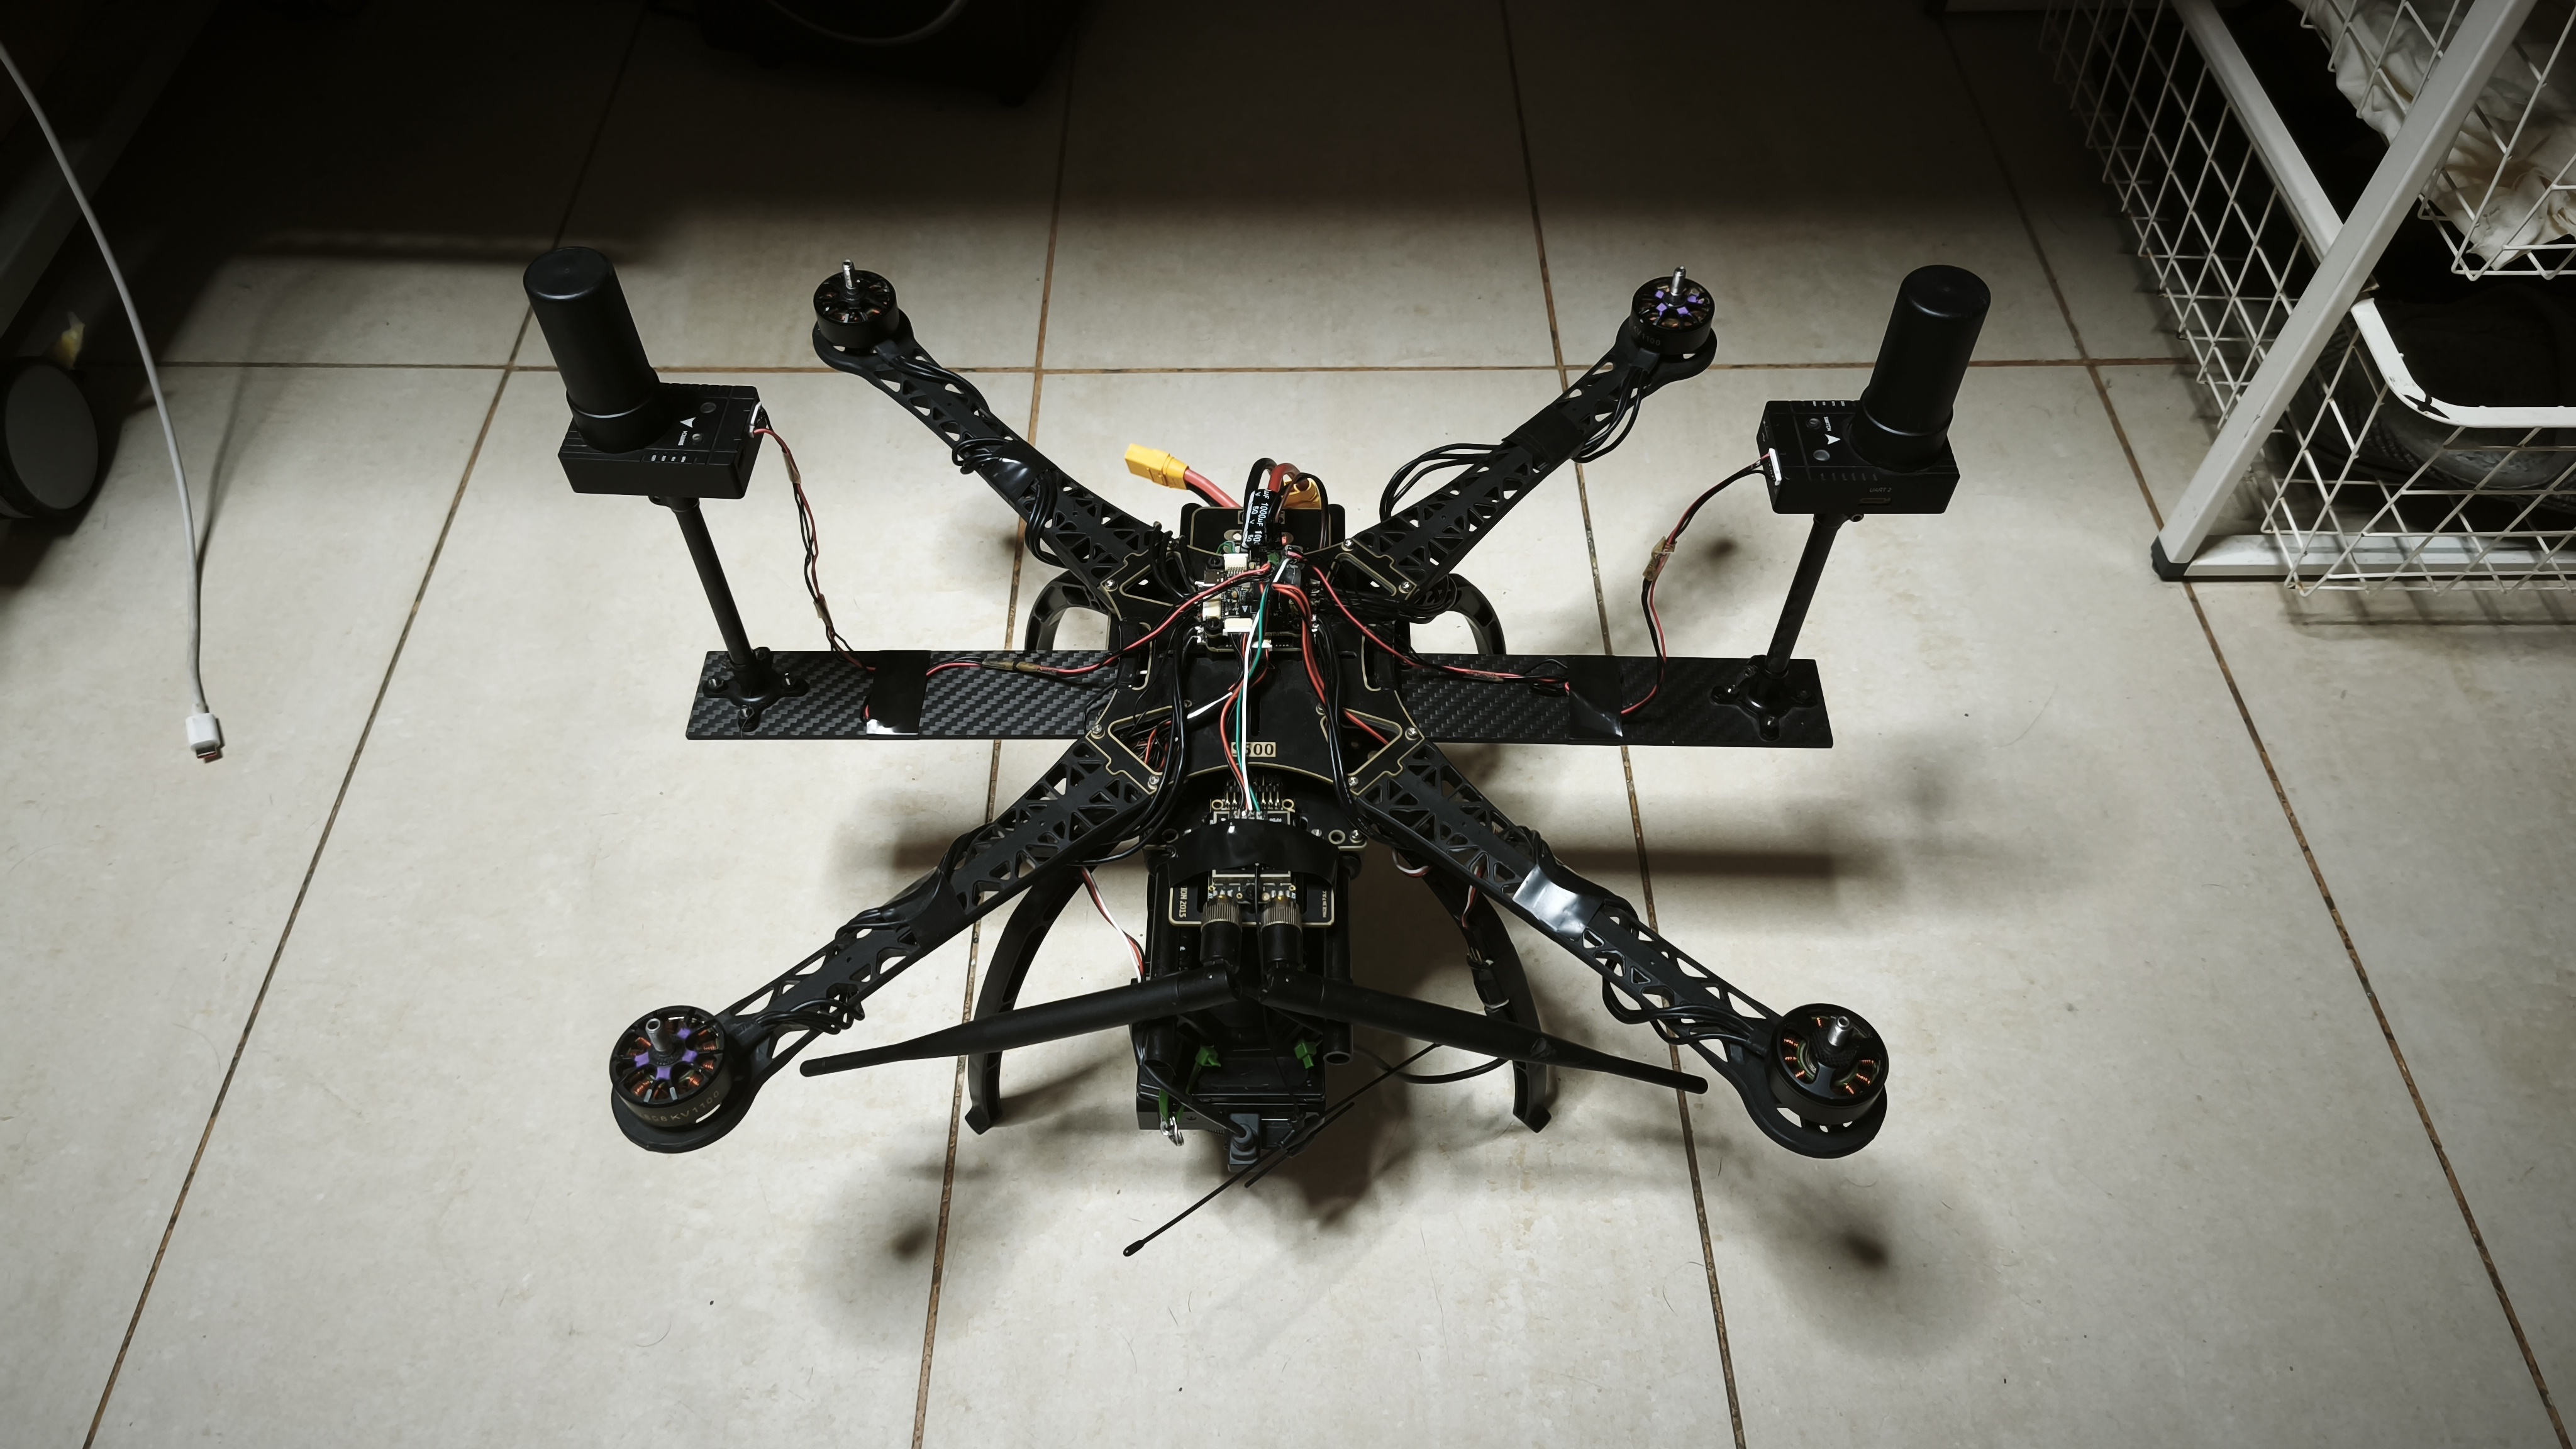
\includegraphics[width=0.75\textwidth]{img/xasis_sencer.jpg}
\end{titlepage}

\chapter*{Resum}
\addcontentsline{toc}{chapter}{Resum}

Aquest document descriu el disseny, la construcció i la posada a punt d'un sistema d'aerofotogrametria de precisió format per tres subsistemes: una base GNSS RTK pròpia, un UAV amb doble receptor GNSS en \emph{moving baseline} i una càmera amb sincronisme de sabata, i una estació de terra que els enllaça. L'objectiu és el geoetiquetat centimètric de les fotografies aèries per generar ortomosaics i models digitals de superfície, amb un cost de maquinari d'uns 2.150~€ i control total sobre el \emph{firmware}, les correccions i el flux de dades.

Els resultats principals són:
\begin{itemize}
    \item Una arquitectura que serveix les correccions RTCM3 per WiFi local i les reenvia al dron per un enllaç de telemetria de llarg abast, i que obté RTK Fixed al 100~\% del vol als dos receptors, amb \emph{yaw} derivat del GNSS i sense brúixola magnètica.
    \item Una campanya de proves de vol que va resoldre, a partir de l'anàlisi dels registres, oscil·lacions de control, una fallada de configuració del \emph{moving baseline}, el col·lapse d'una bateria i els problemes de disparament de la càmera (\cref{chap:proves-vol}).
    \item Dos vols de fotogrametria processats de punta a punta: 118 fotografies reconstruïdes a 30~m, amb un GSD de 0,45~cm/px i un error de reprojecció de 0,90~px, i 110 a 50~m (\cref{chap:vols-prova}).
    \item La mesura, per dos mètodes independents, d'un retard efectiu de l'obturador de 0,27--0,28~s ($\sim$1,3~m a 5~m/s), que justifica el \emph{feedback} de sabata i es compensa al geoetiquetat.
    \item Una anàlisi del grup propulsor que identifica el diàmetre d'hèlix com a factor limitant de l'autonomia i en quantifica el marge de millora (\cref{sec:propulsor}).
\end{itemize}

La precisió del producte final encara no s'ha pogut afirmar: requereix punts de control i de comprovació a terra mesurats amb la mateixa base que el vol, previstos al pla de proves de precisió (\cref{sec:validacio}). Com que la base fa un \emph{survey-in} a cada sessió, la posició absoluta del mapa té un desplaçament de l'ordre de metres que només es pot corregir amb el registre de la base. El document marca amb un requadre \emph{Pendent} la documentació i les proves que encara falten, i la llista consolidada de tasques és a \cref{sec:pendents-proves-vol}.

\tableofcontents

\mainmatter

% =====================================================
% PART I — DISSENY I CONSTRUCCIÓ
% =====================================================
\part{Disseny i construcció}
\chapter{Disseny i construcció del sistema}
\label{chap:construccio}

\section{Introducció}
\label{sec:introduccio}

Aquest document descriu el disseny, la construcció i la validació en vol d'un sistema complet d'aerofotogrametria de precisió (\emph{surveying} amb dron): una base GNSS RTK pròpia, un UAV amb doble receptor GNSS i una càmera amb sincronisme de sabata, i una estació de terra que els enllaça.

L'objectiu és aconseguir geoetiquetat centimètric de les fotografies aèries ($\leq 2$~cm en horitzontal, $\leq 3$~cm en vertical) per generar ortomosaics i models digitals de superfície de qualitat topogràfica, amb un cost total de maquinari al voltant dels 2.150~€ --~una fracció del cost d'un DJI P4 RTK o d'un conjunt Emlid~+~UAV~-- i amb control total sobre el \emph{firmware}, les correccions i el flux de dades.

El sistema es divideix en tres subsistemes:
\begin{itemize}
    \item \textbf{Base GNSS RTK}: estació fixa que genera correccions RTCM3.
    \item \textbf{UAV (\emph{rover})}: dron amb doble receptor GNSS per a posicionament RTK i \emph{heading} per \emph{moving baseline}.
    \item \textbf{Estació de terra (GS)}: enllaç de telemetria i redistribució de correccions cap al dron.
\end{itemize}

El document s'organitza en quatre blocs: el disseny i la construcció (aquest capítol), el manual d'operació i procediments (\cref{chap:manual}), la campanya de proves de vol i posada a punt (\cref{chap:proves-vol}) i els vols de fotogrametria que en resulten (\cref{chap:vols-prova}).

\section{Arquitectura i flux de dades}
\label{sec:arquitectura}

L'arquitectura escollida fa servir la base per servir correccions RTCM3 per WiFi local (mode \emph{access point}) mitjançant un servidor TCP propi, sense NTRIP. Es va descartar l'enllaç ràdio directe base~$\rightarrow$~dron per simplificar el sistema (un sol canal de ràdio al dron) i per guanyar resiliència en zones rurals sense cobertura mòbil.

\begin{figure}[H]
    \centering
    \resizebox{\linewidth}{!}{%
    \begin{tikzpicture}[
        box/.style={draw, rounded corners=2pt, align=center, font=\small, minimum height=10mm, minimum width=27mm, fill=blue!5},
        arr/.style={-{Stealth[length=2mm]}, thick},
        grp/.style={draw, dashed, rounded corners=4pt, inner sep=4mm, gray},
        node distance=8mm and 17mm]
        \node[box] (ant) {Antena\\multibanda};
        \node[box, right=of ant] (f9b) {ZED-F9P\\(base, \emph{survey-in})};
        \node[box, right=of f9b] (pi) {Raspberry Pi\\servidor TCP};
        \node[box, below=16mm of pi] (gs) {Mission Planner\\(estació de terra)};
        \node[box, left=of gs] (rfdg) {RFD868x\\(costat GS)};
        \node[box, below=16mm of rfdg] (rfdu) {RFD868x\\(costat dron)};
        \node[box, right=of rfdu] (fc) {Controlador de vol\\(Kakute H7, EKF3)};
        \node[box, right=of fc] (gnss) {2$\times$ ZED-F9P\\\emph{moving baseline}};
        \node[box, below=10mm of fc] (cam) {Sony $\alpha$6000\\MAP2 + SYNC2};
        \draw[arr] (ant) -- (f9b);
        \draw[arr] (f9b) -- node[above, font=\scriptsize] {RTCM3} (pi);
        \draw[arr] (pi) -- node[right, font=\scriptsize] {WiFi} (gs);
        \draw[arr] (gs) -- node[above, font=\scriptsize] {USB} (rfdg);
        \draw[arr] (rfdg) -- node[right, font=\scriptsize] {868~MHz} (rfdu);
        \draw[arr] (rfdu) -- node[above, font=\scriptsize] {MAVLink} (fc);
        \draw[arr, <->] (fc) -- node[above, font=\scriptsize] {UART} (gnss);
        \draw[arr, <->] (fc) -- node[right, font=\scriptsize] {PWM / sabata} (cam);
        \begin{scope}[on background layer]
            \node[grp, fit=(ant)(f9b)(pi), label={[font=\small, gray]above:Base RTK}] {};
            \node[grp, fit=(rfdu)(fc)(gnss)(cam), label={[font=\small, gray]above:UAV}] {};
        \end{scope}
    \end{tikzpicture}}
    \caption{Diagrama de blocs del sistema i flux de les correccions RTCM3.}
    \label{fig:diagrama-blocs}
\end{figure}

\subsection{Flux complet de dades}

\begin{enumerate}[label=\arabic*.]
    \item L'antena multibanda capta L1/L2/L5 (GPS, GLONASS, Galileo, BeiDou).
    \item El \textbf{ZED-F9P} de la base (mode \emph{survey-in} a cada sessió, \cref{sec:protocol-camp}) genera missatges \textbf{RTCM3} (1005, 1074, 1084, 1094, 1124 i 1230) a 1~Hz. El 1005, amb la posició de la base, només surt quan el \emph{survey-in} és vàlid.
    \item La \textbf{Raspberry Pi} rep aquests missatges per USB (port sèrie del receptor simpleRTK2B Pro) i els redistribueix tal com arriben pel servidor TCP del port 5000, per WiFi AP.
    \item La \textbf{GS} (Mission Planner / QGroundControl al costat del pilot) es connecta al servidor TCP i reenvia el flux RTCM3 al dron per MAVLink (\texttt{GPS\_RTCM\_DATA}) a través del parell \textbf{RFD868x}.
    \item Al dron, el F9P primari rep les correccions, calcula la posició RTK i, en mode \emph{moving baseline}, genera RTCM 4072.x cap al secundari per derivar el \emph{heading}.
    \item El \textbf{FC} integra la posició RTK i el \emph{yaw} GNSS a l'EKF3 per a navegació i geoetiquetat.
\end{enumerate}

\section{Decisions de disseny}
\label{sec:decisions}

\begin{description}
    \item[Moving baseline amb 2$\times$ ZED-F9P] en lloc d'un UM982 amb \emph{heading} natiu. El F9P està més documentat, té més suport comunitari i és intercanviable entre base i UAV. Proporciona GPS-for-yaw, cosa que permet prescindir de la brúixola magnètica --~avantatge important en \emph{frames} amb molt corrent.
    \item[RFD868x per a l'enllaç GS$\leftrightarrow$UAV] als 868~MHz (banda europea) permet fins a 500~mW EIRP i un abast superior a 40~km. Sempre versió europea 868 (mai 915 o 433).
    \item[Servidor TCP local per WiFi] robust en absència de cobertura mòbil; a la pràctica gairebé sempre s'opera en local (aparcar el vehicle, muntar el trípode al costat i volar).
    \item[Retroalimentació de la sabata (Seagull SYNC2)] resol la latència variable de l'obturador ($\sim$100~ms equivalen a 1,5~m d'error a 15~m/s). Sense aquest \emph{feedback} no hi ha precisió centimètrica real al geoetiquetat; \cref{sec:retard-obturador} en quantifica l'efecte.
    \item[Post-procés PPK opcional] enregistrament de dades \texttt{UBX} en brut a la base i al dron, que permet obtenir una solució independent de la qualitat de l'enllaç RTK en temps real.
\end{description}

\section{Llista de materials}
\label{sec:materials}

El maquinari del sistema suposa un cost total de 2150~€.

\subsection{Dron}

\begin{table}[H]
    \centering
    \caption{Components del dron (UAV/\emph{rover})}
    \label{tab:materials-dron}
    \begin{tabular}{lll}
        \toprule
        Component & Model & Cost aprox. \\
        \midrule
        \emph{Frame} & S500 (Quad X, 500~mm entre eixos) & 35~€ \\
        Motors (4$\times$) & Pilotix 2808, 1100~KV & 60~€ \\
        ESC & Hobbywing XRotor 65A 4-in-1 (DShot) & 30~€ \\
        FC & Holybro Kakute H7 (STM32H7) & 55~€ \\
        GPS (2$\times$) & Holybro H-RTK F9P Helical & 510~€ (255~€/u) \\
        Telemetria & RFD868x EU 500~mW (parell dron + GS) & 363~€ \\
        RC & Radiomaster XR1 Nano ELRS dual-band & 16~€ \\
        Bateria & Gaoneng GNB 6S 4000~mAh 70C & 70~€ \\
        \bottomrule
    \end{tabular}
\end{table}

\begin{description}
    \item[Motors Pilotix 2808, 1100~KV] KV moderat per a 6S, pensat per a hèlixs de 8~polzades (\cref{tab:kv-compatibilitat}) amb la càrrega útil addicional del sistema RTK~+~càmera, en lloc dels KV alts típics de \emph{freestyle}, que sacrifiquen eficiència per velocitat. Les hèlixs de 7~polzades del muntatge inicial van ser per disponibilitat, no per disseny (\cref{subsec:propulsor-inicial}).
    \item[ESC Hobbywing XRotor 65A 4-in-1 (DShot)] marge de corrent per al pes addicional; el DShot bidireccional permet telemetria de RPM per motor, útil per a diagnòstic de vibracions; el format 4-in-1 simplifica el cablejat de potència.
    \item[FC Holybro Kakute H7 (STM32H7)] prou ports UART per a tota l'arquitectura sense necessitat d'expansió (2$\times$F9P, RFD868x, RC ELRS, telemetria ESC, USB) i suport natiu a ArduPilot per a GPS \emph{moving baseline} i DShot.
    \item[GPS Holybro H-RTK F9P Helical (2$\times$)] mòdul integrat (antena helical + \emph{breakout} F9P) ja pensat per a \emph{moving baseline} amb ArduPilot; evita haver de dissenyar i aparellar antena i \emph{breakout} per separat.
    \item[Telemetria RFD868x] justificació completa a \cref{sec:decisions}.
    \item[RC Radiomaster XR1 Nano ELRS] mida i pes mínims per no penalitzar la càrrega útil; ELRS de baixa latència complementa el RFD868x, que porta les dades MAVLink/RTCM però no el control de vol.
    \item[Bateria Gaoneng 6S 4000~mAh 70C] 6S per millor eficiència de tensió amb el consum addicional (GPS, telemetria, càmera); 70C dona marge de corrent de pic suficient amb els 4 motors a plena càrrega.
\end{description}

\subsection{Base GNSS}

\begin{table}[H]
    \centering
    \caption{Components de la base RTK}
    \label{tab:materials-base}
    \begin{tabular}{lll}
        \toprule
        Component & Model & Cost aprox. \\
        \midrule
        GNSS & ArduSimple simpleRTK2B Pro (ZED-F9P) & 126~€ \\
        Antena & BD900 GNSS (multibanda) & 43~€ \\
        SBC & Raspberry Pi Zero W & 35~€ \\
        Alimentació & Waveshare UPS HAT + 2$\times$ 18650 3500~mAh & 47~€ \\
        \bottomrule
    \end{tabular}
\end{table}

\begin{description}
    \item[GNSS simpleRTK2B Pro (ZED-F9P)] placa de desenvolupament amb USB i connector d'antena SMA, amb el mateix xip que els receptors del dron, cosa que dona intercanviabilitat i una configuració i un \emph{firmware} compartits (\cref{sec:decisions}).
    \item[Antena BD900 GNSS (multibanda)] necessària per rebre les dues bandes i les múltiples constel·lacions que fa servir el ZED-F9P, requisit perquè el \emph{survey-in} convergeixi (\cref{sec:protocol-camp}).
    \item[Raspberry Pi Zero W] mida i consum reduïts per a ús en camp amb bateria, amb prou capacitat per distribuir les correccions pel servidor TCP i fer de punt d'accés WiFi (NetworkManager).
    \item[Alimentació UPS HAT + 2$\times$18650] autonomia de la base independent de la xarxa elèctrica al camp, amb protecció davant talls durant l'enregistrament.
\end{description}

\subsection{Estació de terra}

\begin{table}[H]
    \centering
    \caption{Components de l'estació de terra (GS)}
    \label{tab:materials-gs}
    \begin{tabular}{lll}
        \toprule
        Component & Model & Cost aprox. \\
        \midrule
        Comandament & Radiomaster TX16S (o similar) ELRS & 167~€ \\
        Telemetria & RFD868x (costat GS, inclòs al parell) & -- \\
        Portàtil / tauleta & Propi, amb Mission Planner & -- \\
        \bottomrule
    \end{tabular}
\end{table}

El comandament i el parell RFD868x són elements estàndard sense decisió específica de disseny. L'únic element addicional de la GS és el portàtil o la tauleta amb Mission Planner o QGroundControl, que fa de pont entre el servidor TCP de la base i el flux MAVLink cap al dron (\cref{sec:arquitectura}).

\subsection{Càmera (mòdul de cartografia)}

\begin{table}[H]
    \centering
    \caption{Mòdul de càmera per a fotogrametria}
    \label{tab:materials-camera}
    \begin{tabular}{lll}
        \toprule
        Component & Model & Cost aprox. \\
        \midrule
        Cos & Sony $\alpha$6000 (24~MP APS-C, segona mà) & 200~€ \\
        Òptica & TTArtisan 25~mm f/2 APS-C, enfocament manual & 71~€ \\
        \emph{Trigger} & Seagull MAP2 (dispar per PWM) & 30~€ \\
        \emph{Feedback} & Seagull SYNC2 (sabata, X-sync $\rightarrow$ FC) & 30~€ \\
        Targeta SD & 3$\times$ SanDisk Extreme 64~GB & 45~€ \\
        \bottomrule
    \end{tabular}
\end{table}

\begin{description}
    \item[Cos Sony $\alpha$6000] sensor APS-C gran (bona relació senyal/soroll) amb resolució de 24~MP, en un cos i un pes raonables per anar al dron; segona mà per contenir el cost.
    \item[TTArtisan 25~mm f/2] focal curta per a un camp de visió ample (més cobertura per pas de vol i menys passades necessàries) i prou lluminositat per a exposicions curtes. L'enfocament manual permet fixar el focus a infinit i evita que l'autofocus busqui durant el vol, rellevant per a fotogrametria. Construcció metàl·lica compacta i lleugera, amb un cost molt inferior al d'una òptica nativa.
    \item[\emph{Trigger} Seagull MAP2] dispar remot per PWM des del FC sense haver de modificar electrònicament la càmera.
    \item[\emph{Feedback} Seagull SYNC2] obligatori per a la precisió centimètrica del geoetiquetat; justificació a \cref{sec:decisions}.
\end{description}

\subsection{Extres i consumibles}

Cables JST-GH, connectors XT60/XT90, \emph{standoffs} M3, \emph{bracket} de carboni per als helicals, trípode topogràfic de rosca 5/8~polzades, coaxial LMR-240, connectors TNC/SMA amb protecció IP54, targetes microSD i eines (soldador, crimpadora JST-GH, multímetre), amb un cost total d'uns 218~€.

\section{Muntatge}
\label{sec:muntatge}

\subsection{Dron (UAV)}
\label{subsec:muntatge-dron}

El dron es construeix sobre un \emph{frame} S500 en configuració X de 500~mm entre eixos. A la placa central es munta una platina de carboni lateral que fa de \emph{bracket} de \emph{baseline}: a cada extrem hi ha un pal vertical de carboni que porta un mòdul Holybro H-RTK F9P Helical, de manera que les dues antenes queden paral·leles, apuntant amunt i al punt més alt de l'aeronau (\cref{fig:xassis-base}). La separació entre antenes és de 0,38~m sobre l'eix lateral del dron (\cref{sec:antenes-gnss}). El mòdul de telemetria RFD868x, amb les seves dues antenes, es fixa sobre la placa superior i es connecta al controlador de vol per UART.

\begin{figure}[H]
    \centering
    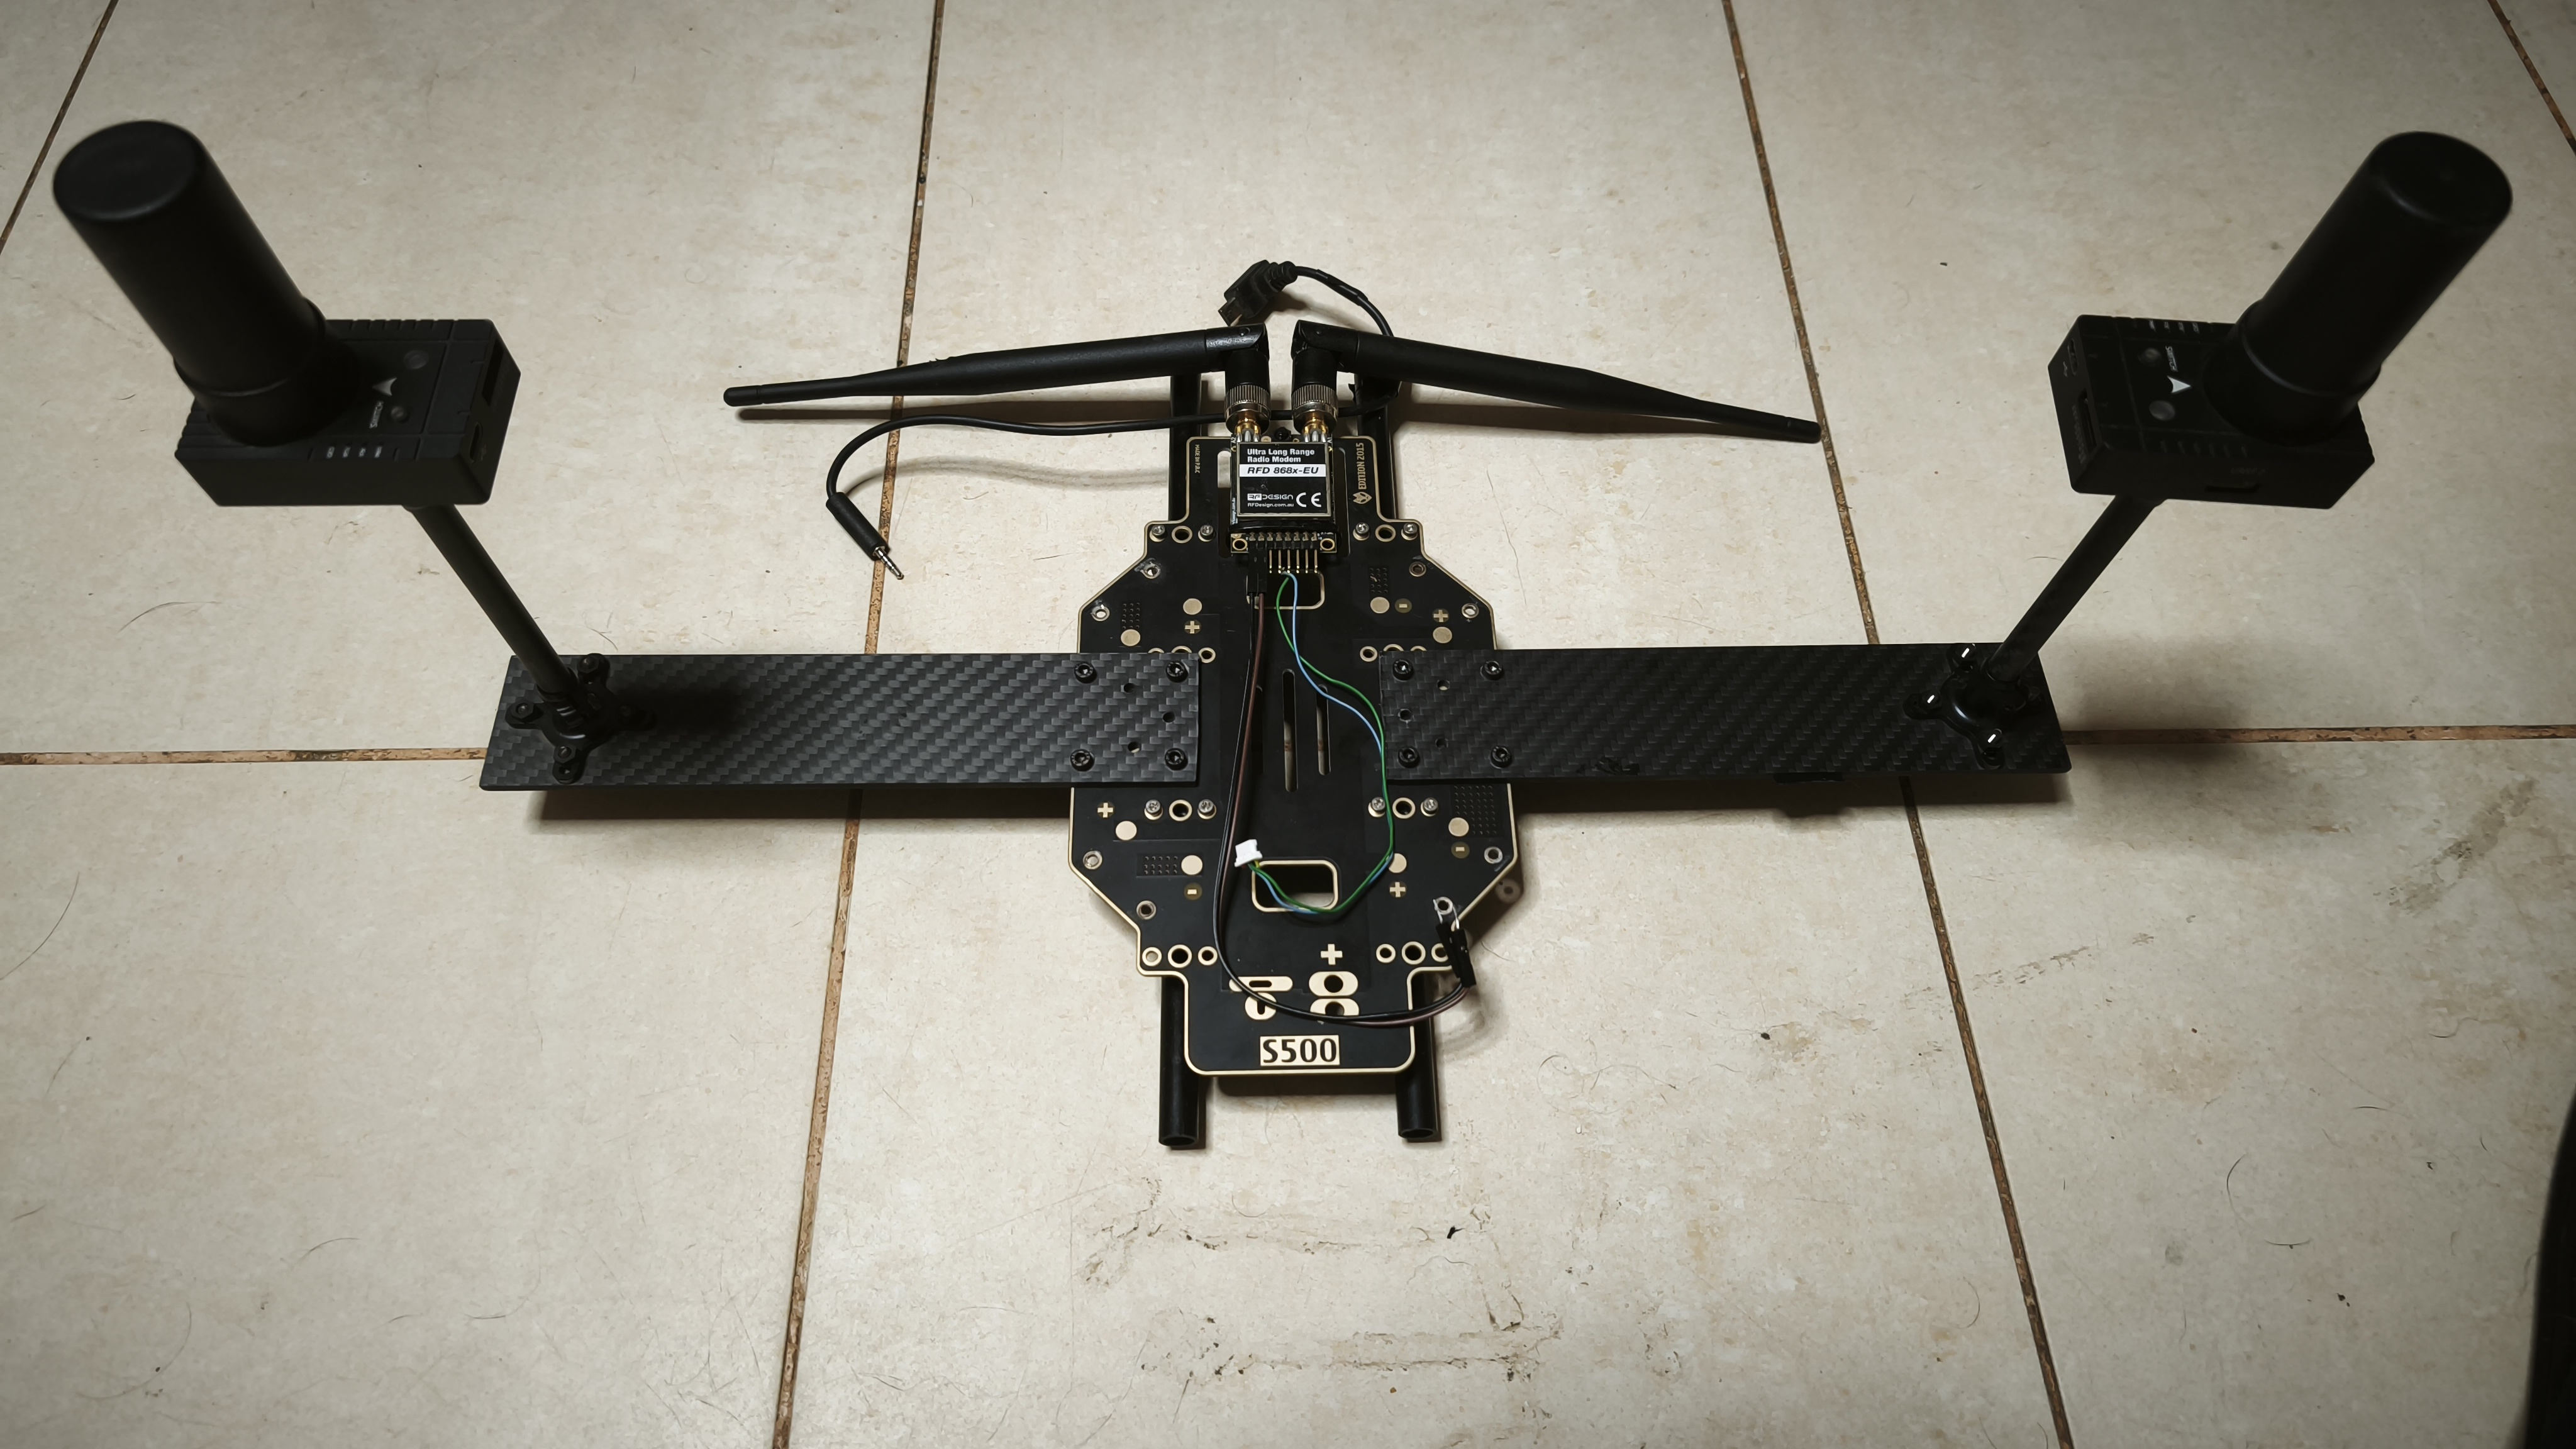
\includegraphics[width=\textwidth]{img/xasis_base.jpg}
    \caption{Placa central S500 amb el \emph{bracket} de carboni, els dos mòduls H-RTK F9P Helical sobre pals verticals i el mòdul RFD868x.}
    \label{fig:xassis-base}
\end{figure}

\begin{figure}[H]
    \centering
    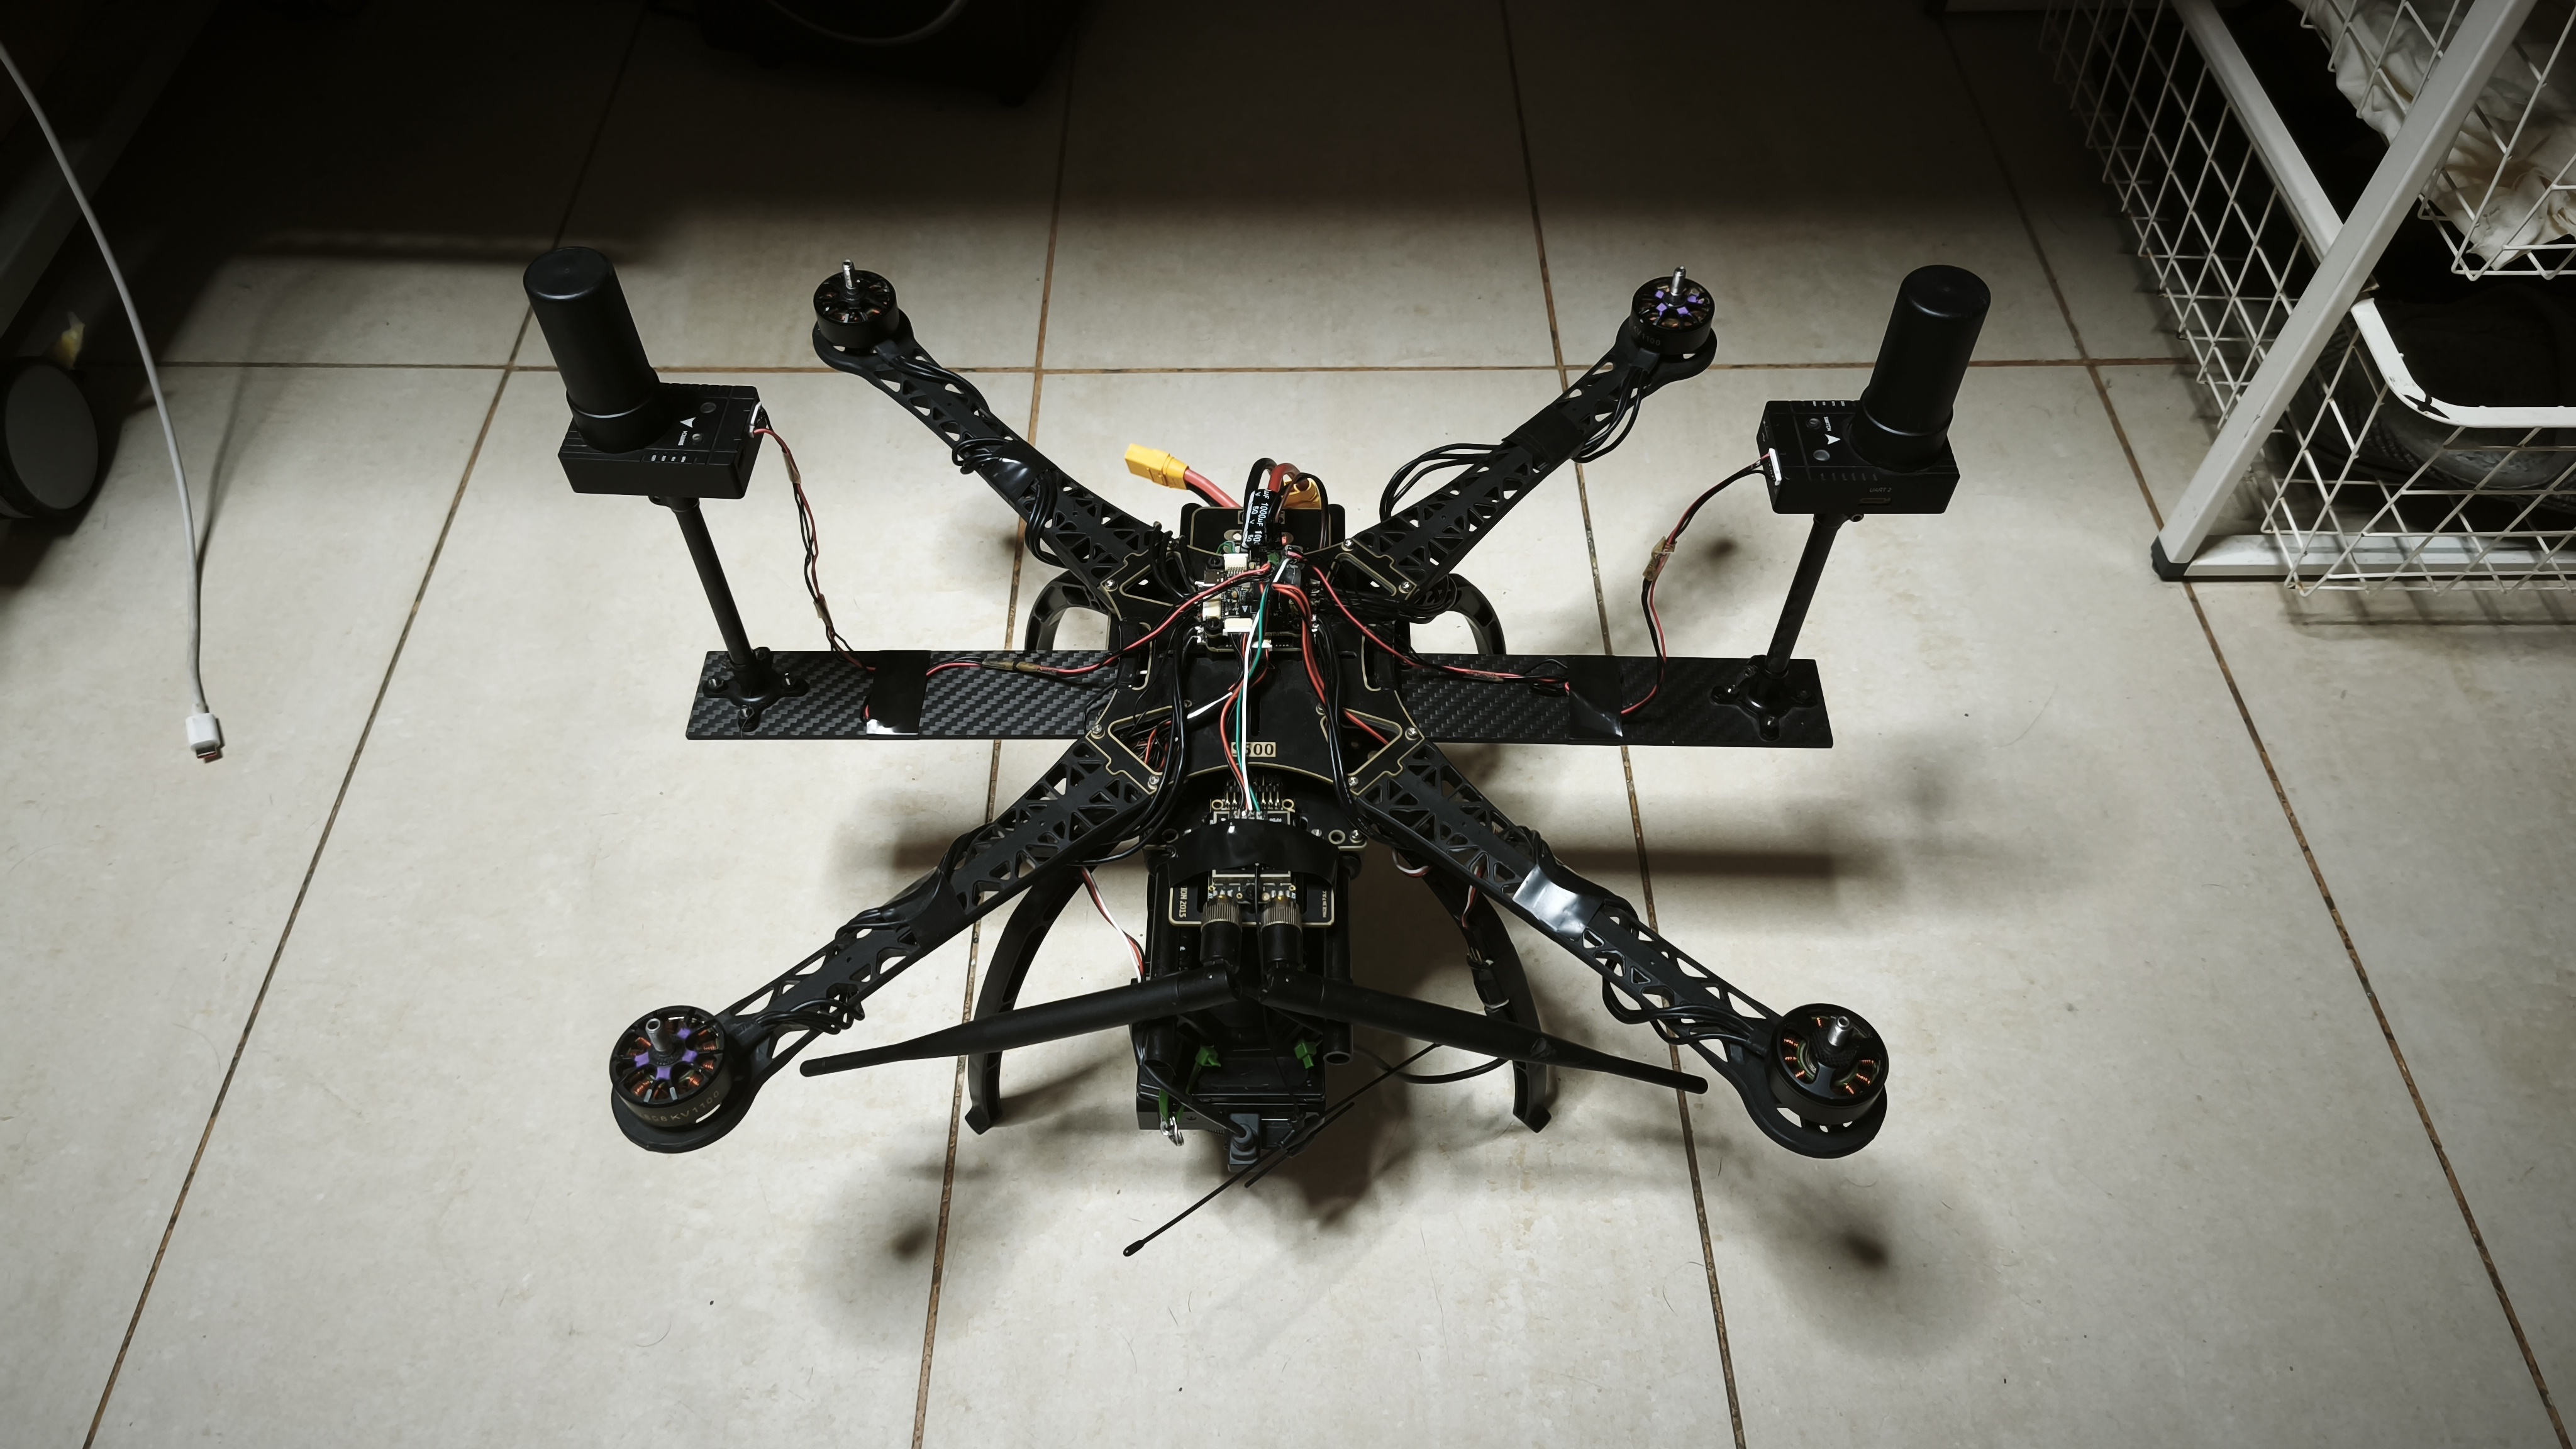
\includegraphics[width=\textwidth]{img/xasis_sencer.jpg}
    \caption{Dron acabat, vist des de dalt: motors, \emph{baseline} lateral amb les dues antenes GNSS, mòdul de telemetria i tren d'aterratge.}
    \label{fig:xassis-sencer}
\end{figure}

Sota el \emph{frame} hi ha un carril format per dues barres de carboni paral·leles amb abraçadores (\cref{fig:xassis-abaix}), que serveix de suport alhora per a la càmera i per a la bateria. La càmera (Sony $\alpha$6000 amb l'òptica de 25~mm) va a nadir, amb el Seagull SYNC2 a la sabata; la bateria 6S es subjecta al mateix carril, de manera que el centre de gravetat queda a prop de l'eix vertical del dron.

\begin{figure}[H]
    \centering
    \begin{subfigure}[b]{0.49\textwidth}
        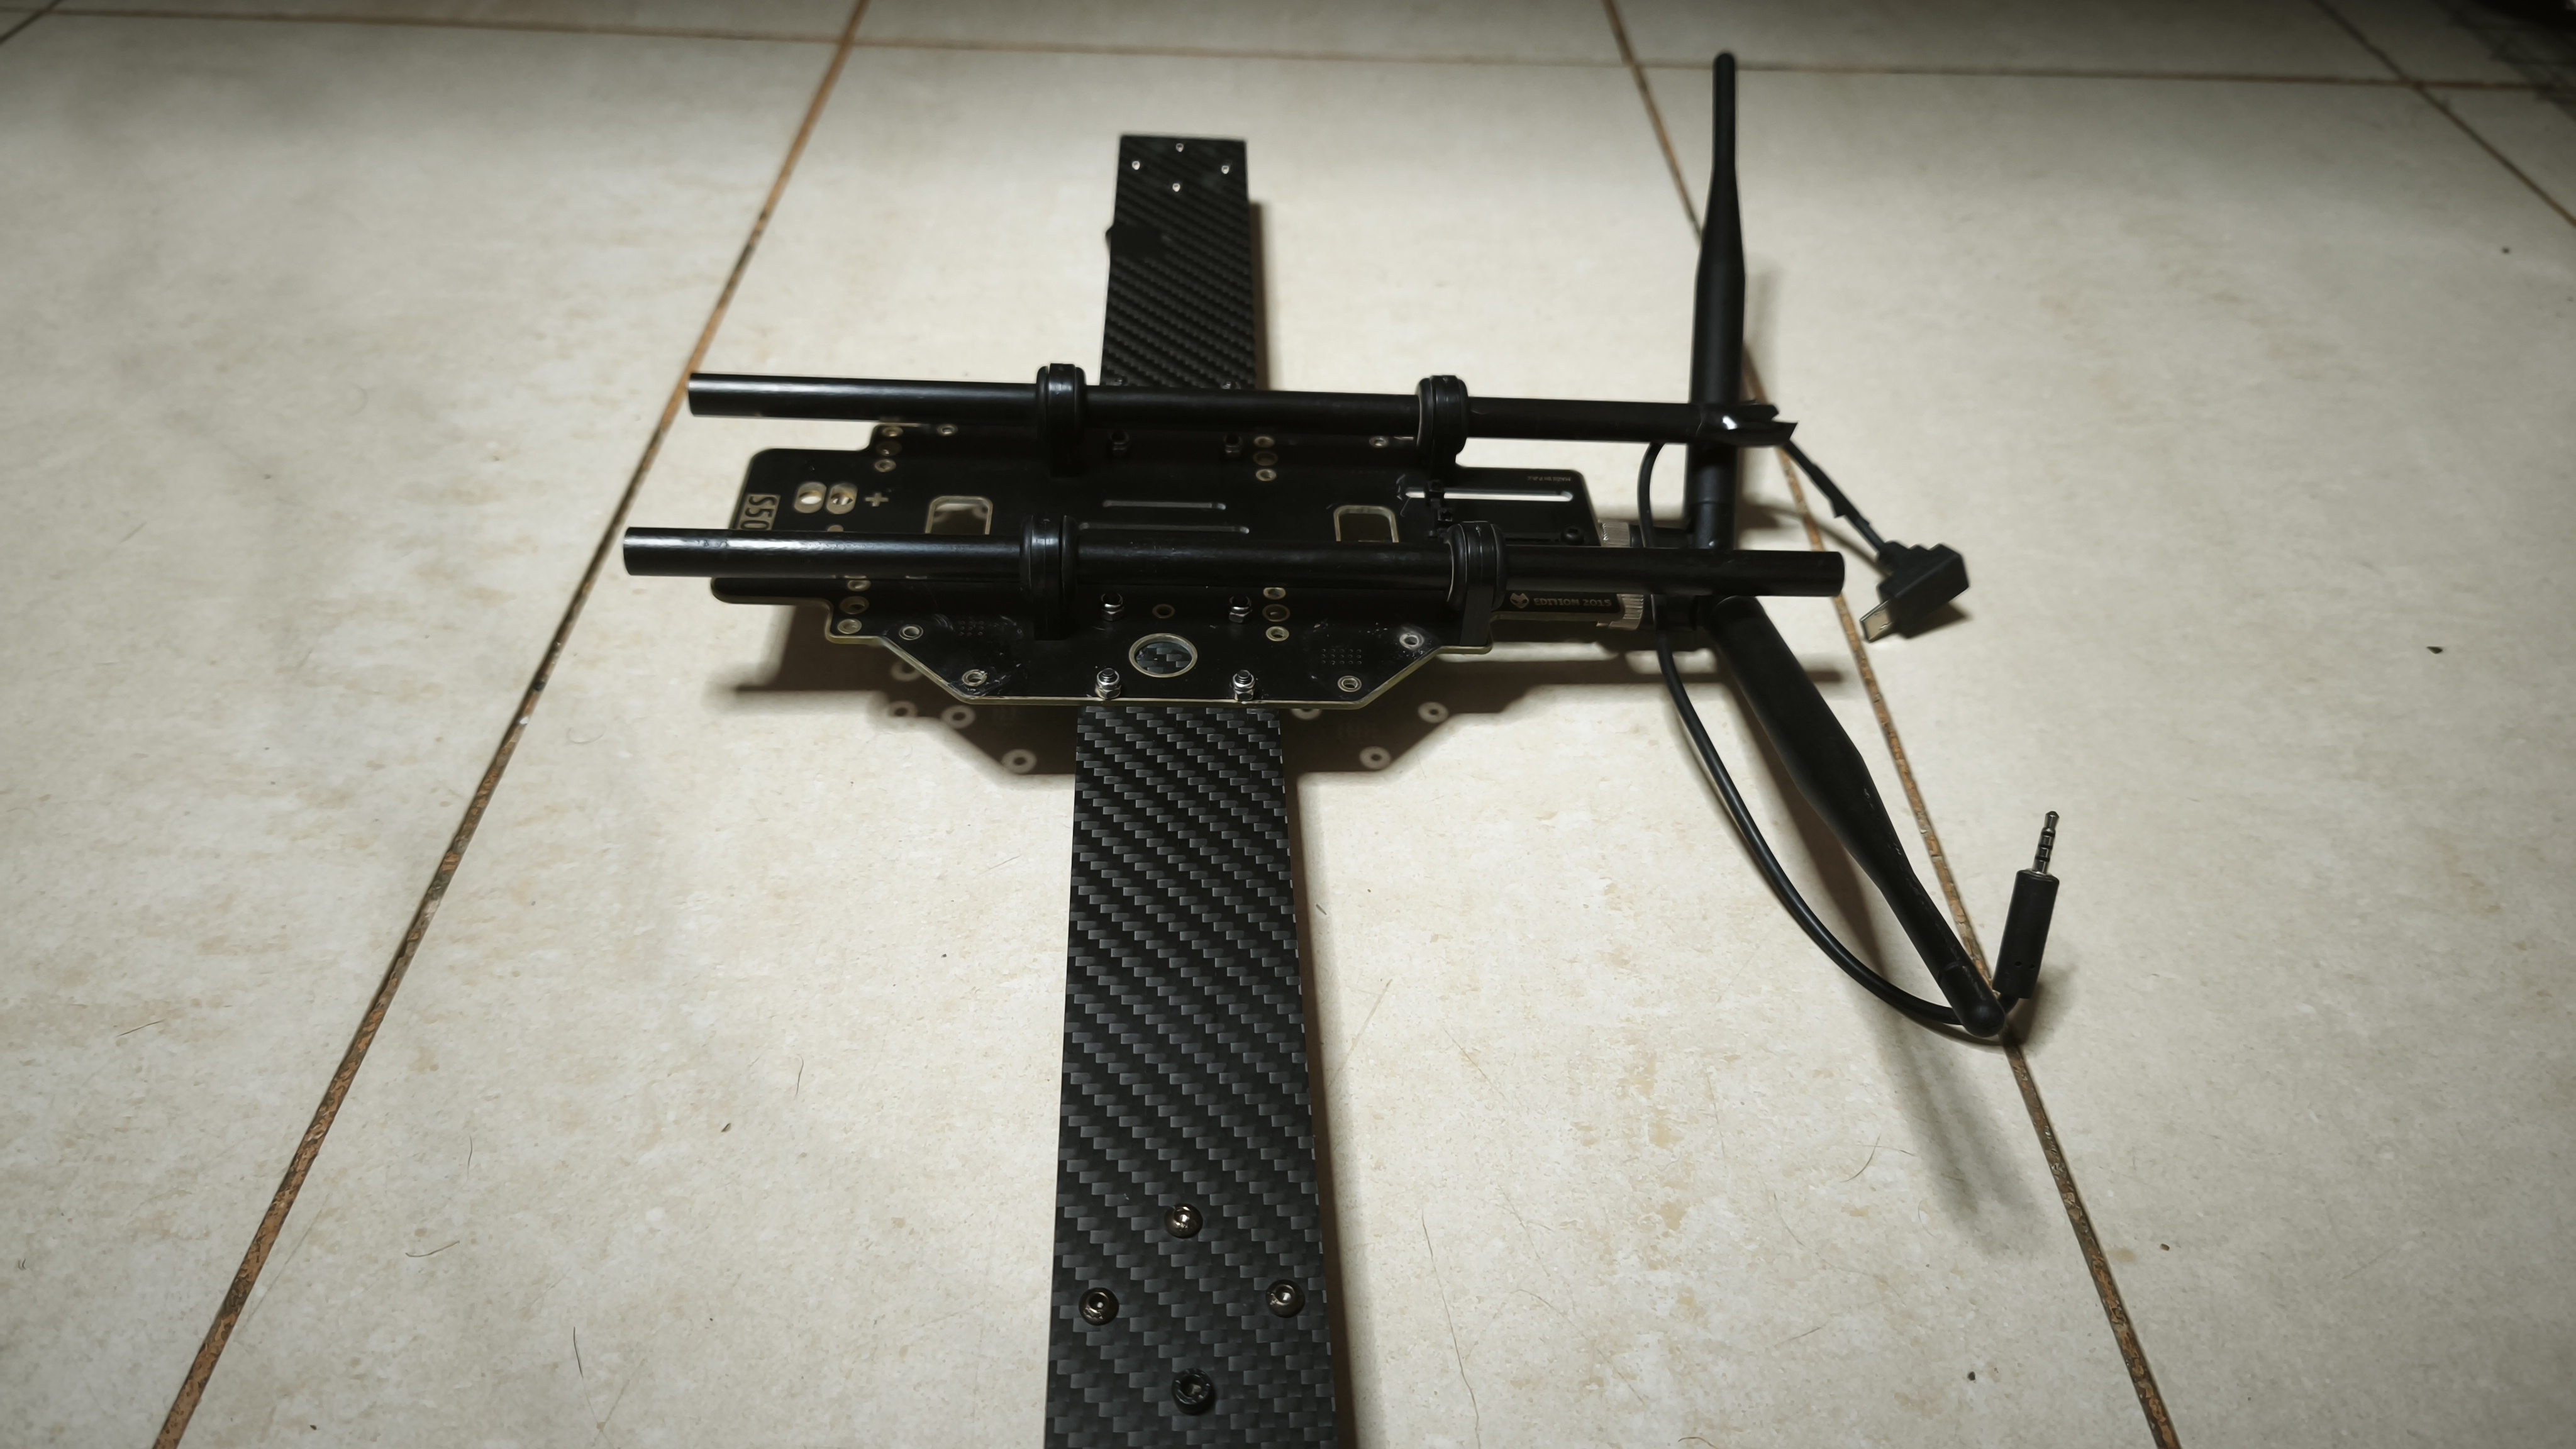
\includegraphics[width=\textwidth]{img/xasis_abaix_buit.jpg}
        \caption{Carril inferior sense càrrega.}
    \end{subfigure}
    \hfill
    \begin{subfigure}[b]{0.49\textwidth}
        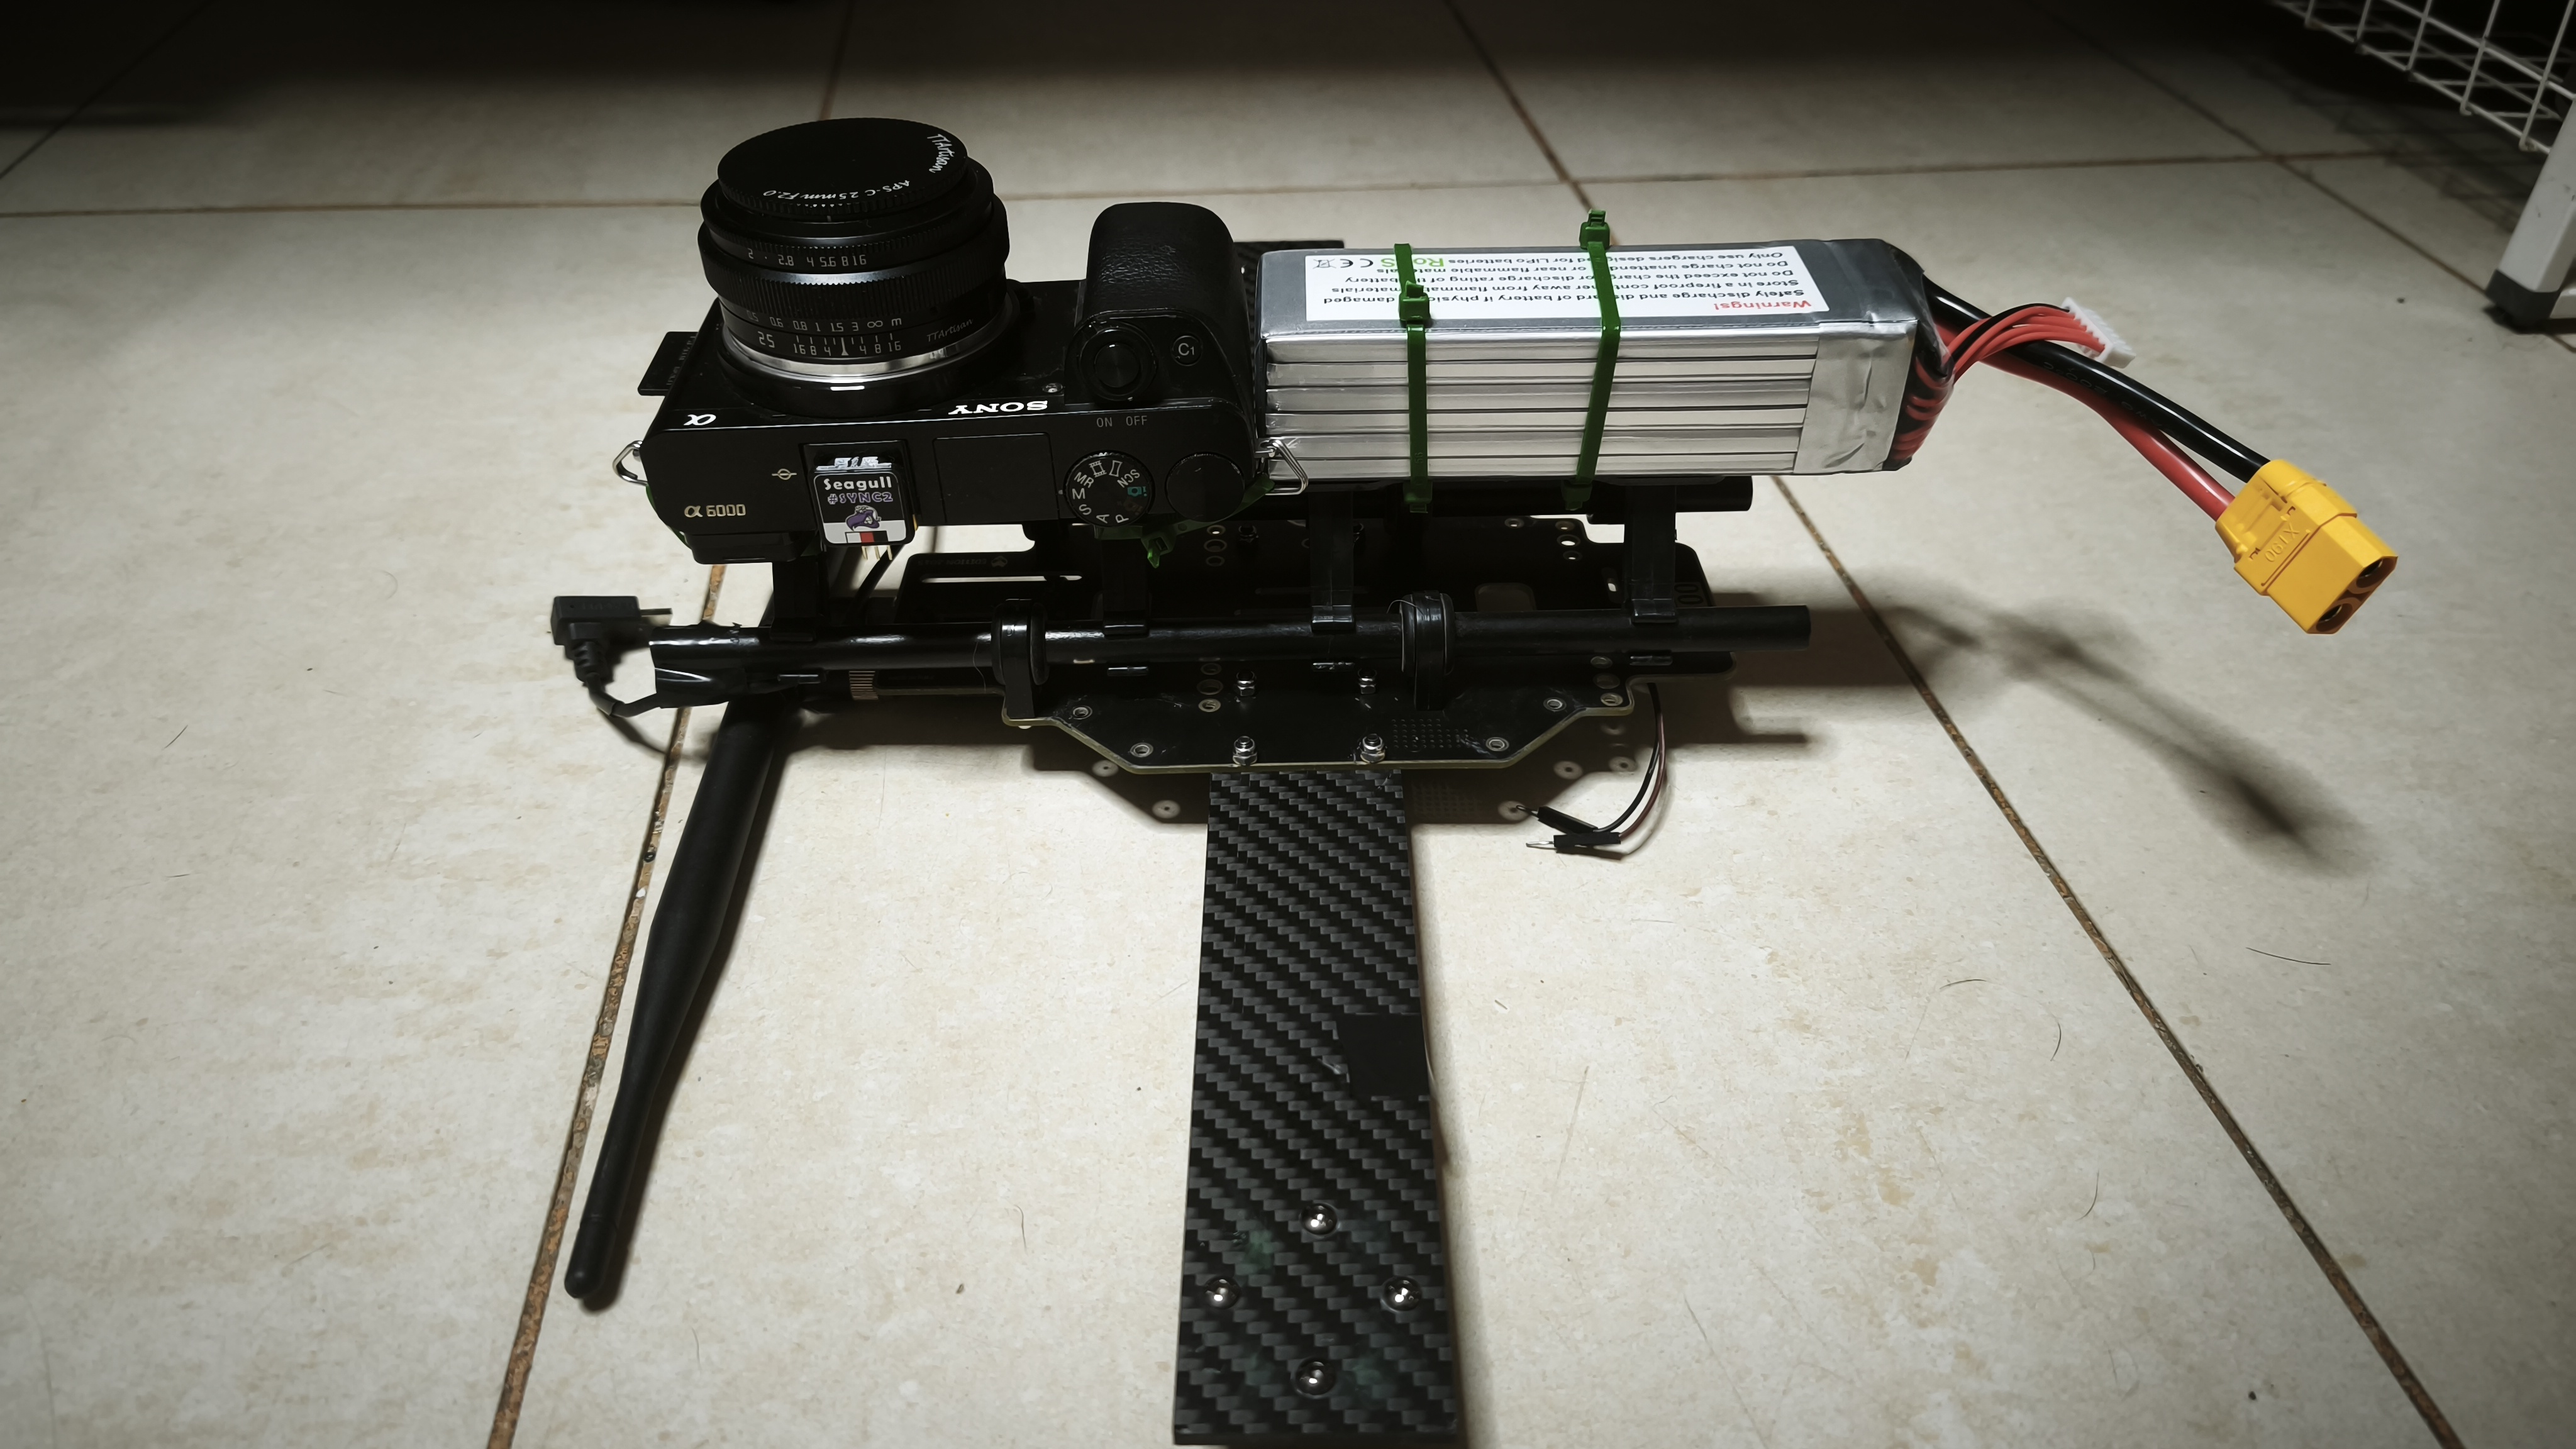
\includegraphics[width=\textwidth]{img/xasis_abaix_ple.jpg}
        \caption{Amb la càmera, el SYNC2 i la bateria.}
    \end{subfigure}
    \caption{Vista inferior del \emph{frame} (girat): carril de carboni i mòdul de càmera.}
    \label{fig:xassis-abaix}
\end{figure}

La configuració dels ports sèrie del FC i els paràmetres de \emph{firmware} (càmera, GPS \emph{moving baseline}) es descriuen al manual d'operació (\cref{chap:manual}).

\subsubsection*{Connexions elèctriques}

\Cref{fig:connexions} mostra el cablejat del dron i \cref{tab:connexions} el resumeix pad a pad. Tots els dispositius es connecten directament a pads del controlador de vol; cap receptor GNSS comparteix cable amb l'altre (el flux del \emph{moving baseline} passa pel controlador, \cref{subsec:gps-moving-baseline}).

\begin{figure}[p]
    \centering
    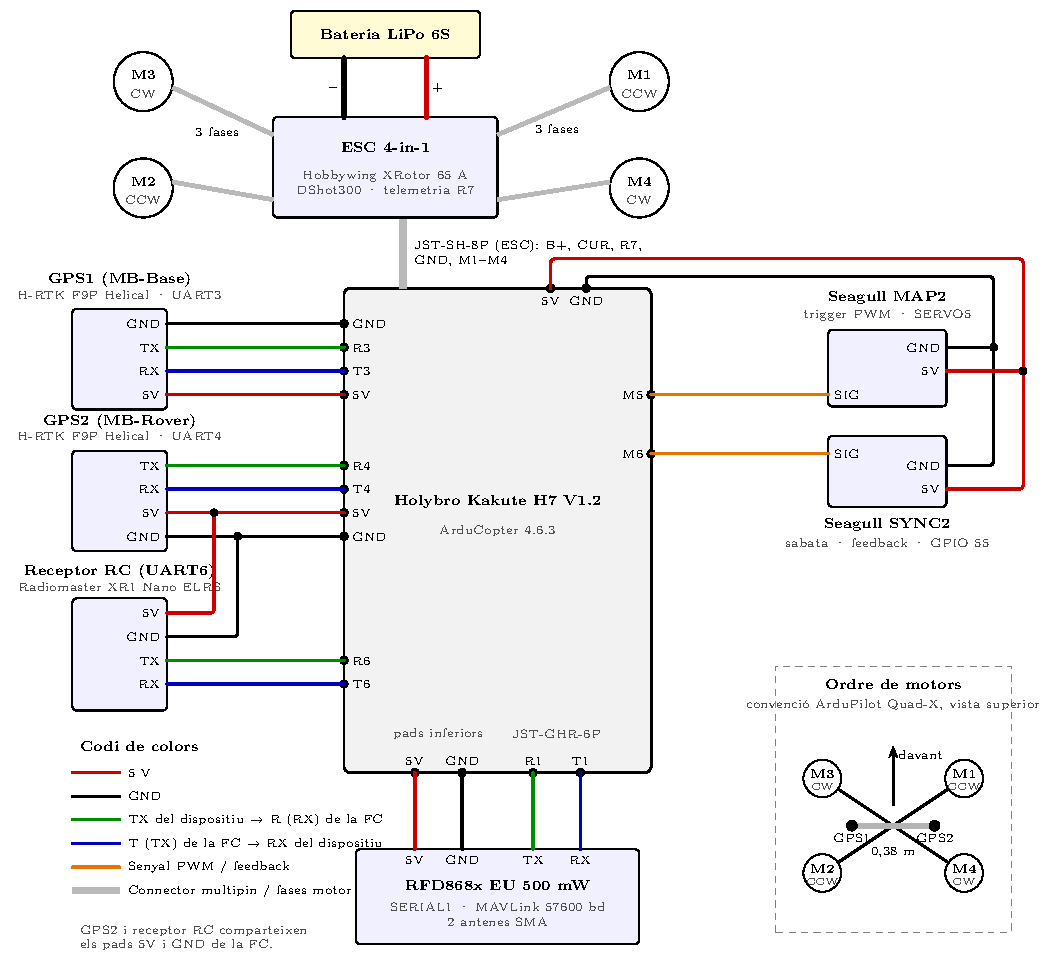
\includegraphics[width=\textwidth]{img/diagrama_connexions.pdf}
    \caption{Esquema de connexions del dron. Els colors segueixen el codi de la llegenda: verd per a la línia TX del dispositiu cap a l'RX de la FC i blau per a la TX de la FC cap a l'RX del dispositiu.}
    \label{fig:connexions}
\end{figure}

\begin{table}[H]
    \centering
    \caption{Connexions del controlador de vol (Kakute H7 V1.2)}
    \label{tab:connexions}
    \small
    \begin{tabular}{P{3.2cm}P{3.9cm}P{3.5cm}P{2.6cm}}
        \toprule
        Dispositiu & Pads de la FC & Funció & Port ArduPilot \\
        \midrule
        GPS1 (MB-Base) & R3, T3, 5V, GND & UART & \texttt{SERIAL3} \\
        GPS2 (MB-Rover) & R4, T4, 5V, GND & UART & \texttt{SERIAL4} \\
        Receptor ELRS & R6, T6, 5V, GND & UART (CRSF) & \texttt{SERIAL6} \\
        RFD868x & R1, T1 (JST-GHR-6P); 5V, GND & UART (MAVLink) & \texttt{SERIAL1} \\
        ESC 4-in-1 & JST-SH-8P: B+, CUR, R7, GND, M1--M4 & DShot, tensió, corrent, telemetria & \texttt{SERIAL7} \\
        Seagull MAP2 & M5; 5V, GND & PWM de \emph{trigger} & \texttt{SERVO5} \\
        Seagull SYNC2 & M6; 5V, GND & \emph{feedback} de la sabata & \texttt{SERVO6} (GPIO 55) \\
        \bottomrule
    \end{tabular}
\end{table}

\subsection{Base GNSS}
\label{subsec:muntatge-base}

La base és una pila compacta de tres plaques fixada a una pota del trípode amb brides (\cref{fig:base}): el receptor ArduSimple simpleRTK2B Pro (amb el ZED-F9P), la Raspberry Pi Zero W i el Waveshare UPS HAT amb les dues bateries 18650. L'antena BD900 GNSS es munta anivellada, amb pla de massa, sobre la rosca 5/8~polzades del trípode topogràfic, a una alçada de 122~cm als vols de prova.

Les connexions són (\cref{fig:base-connexions}):
\begin{itemize}
    \item \textbf{Antena $\rightarrow$ simpleRTK2B Pro:} cable coaxial amb connector SMA.
    \item \textbf{simpleRTK2B Pro $\rightarrow$ Raspberry Pi:} un cable USB-C, que porta les dades (correccions RTCM3 i configuració del receptor) i alimenta el receptor des de la Pi.
    \item \textbf{UPS HAT $\rightarrow$ Raspberry Pi:} només els pins de potència de la capçalera de la Pi es connecten al UPS HAT, que és qui l'alimenta amb les bateries; no hi ha cap línia de comunicació entre tots dos.
\end{itemize}

\begin{figure}[H]
    \centering
    \begin{tikzpicture}[box/.style={draw, rounded corners=2pt, align=center, font=\small, minimum height=10mm, minimum width=22mm, fill=blue!5},
        arr/.style={-{Stealth[length=2mm]}, thick}, node distance=17mm]
        \node[box] (ant) {Antena\\multibanda};
        \node[box, right=of ant] (rtk) {simpleRTK2B Pro\\(ZED-F9P)};
        \node[box, right=of rtk] (pi) {Raspberry Pi\\Zero W};
        \node[box, right=of pi] (ups) {UPS HAT\\2$\times$18650};
        \draw[arr] (ant) -- node[above, font=\scriptsize] {coaxial SMA} (rtk);
        \draw[arr] (rtk) -- node[above, font=\scriptsize] {USB-C} (pi);
        \draw[arr] (ups) -- node[above, font=\scriptsize] {pins 5~V} (pi);
    \end{tikzpicture}
    \caption{Connexions de la base RTK: antena, receptor, SBC i alimentació.}
    \label{fig:base-connexions}
\end{figure}

\begin{figure}[H]
    \centering
    \begin{subfigure}[b]{0.43\textwidth}
        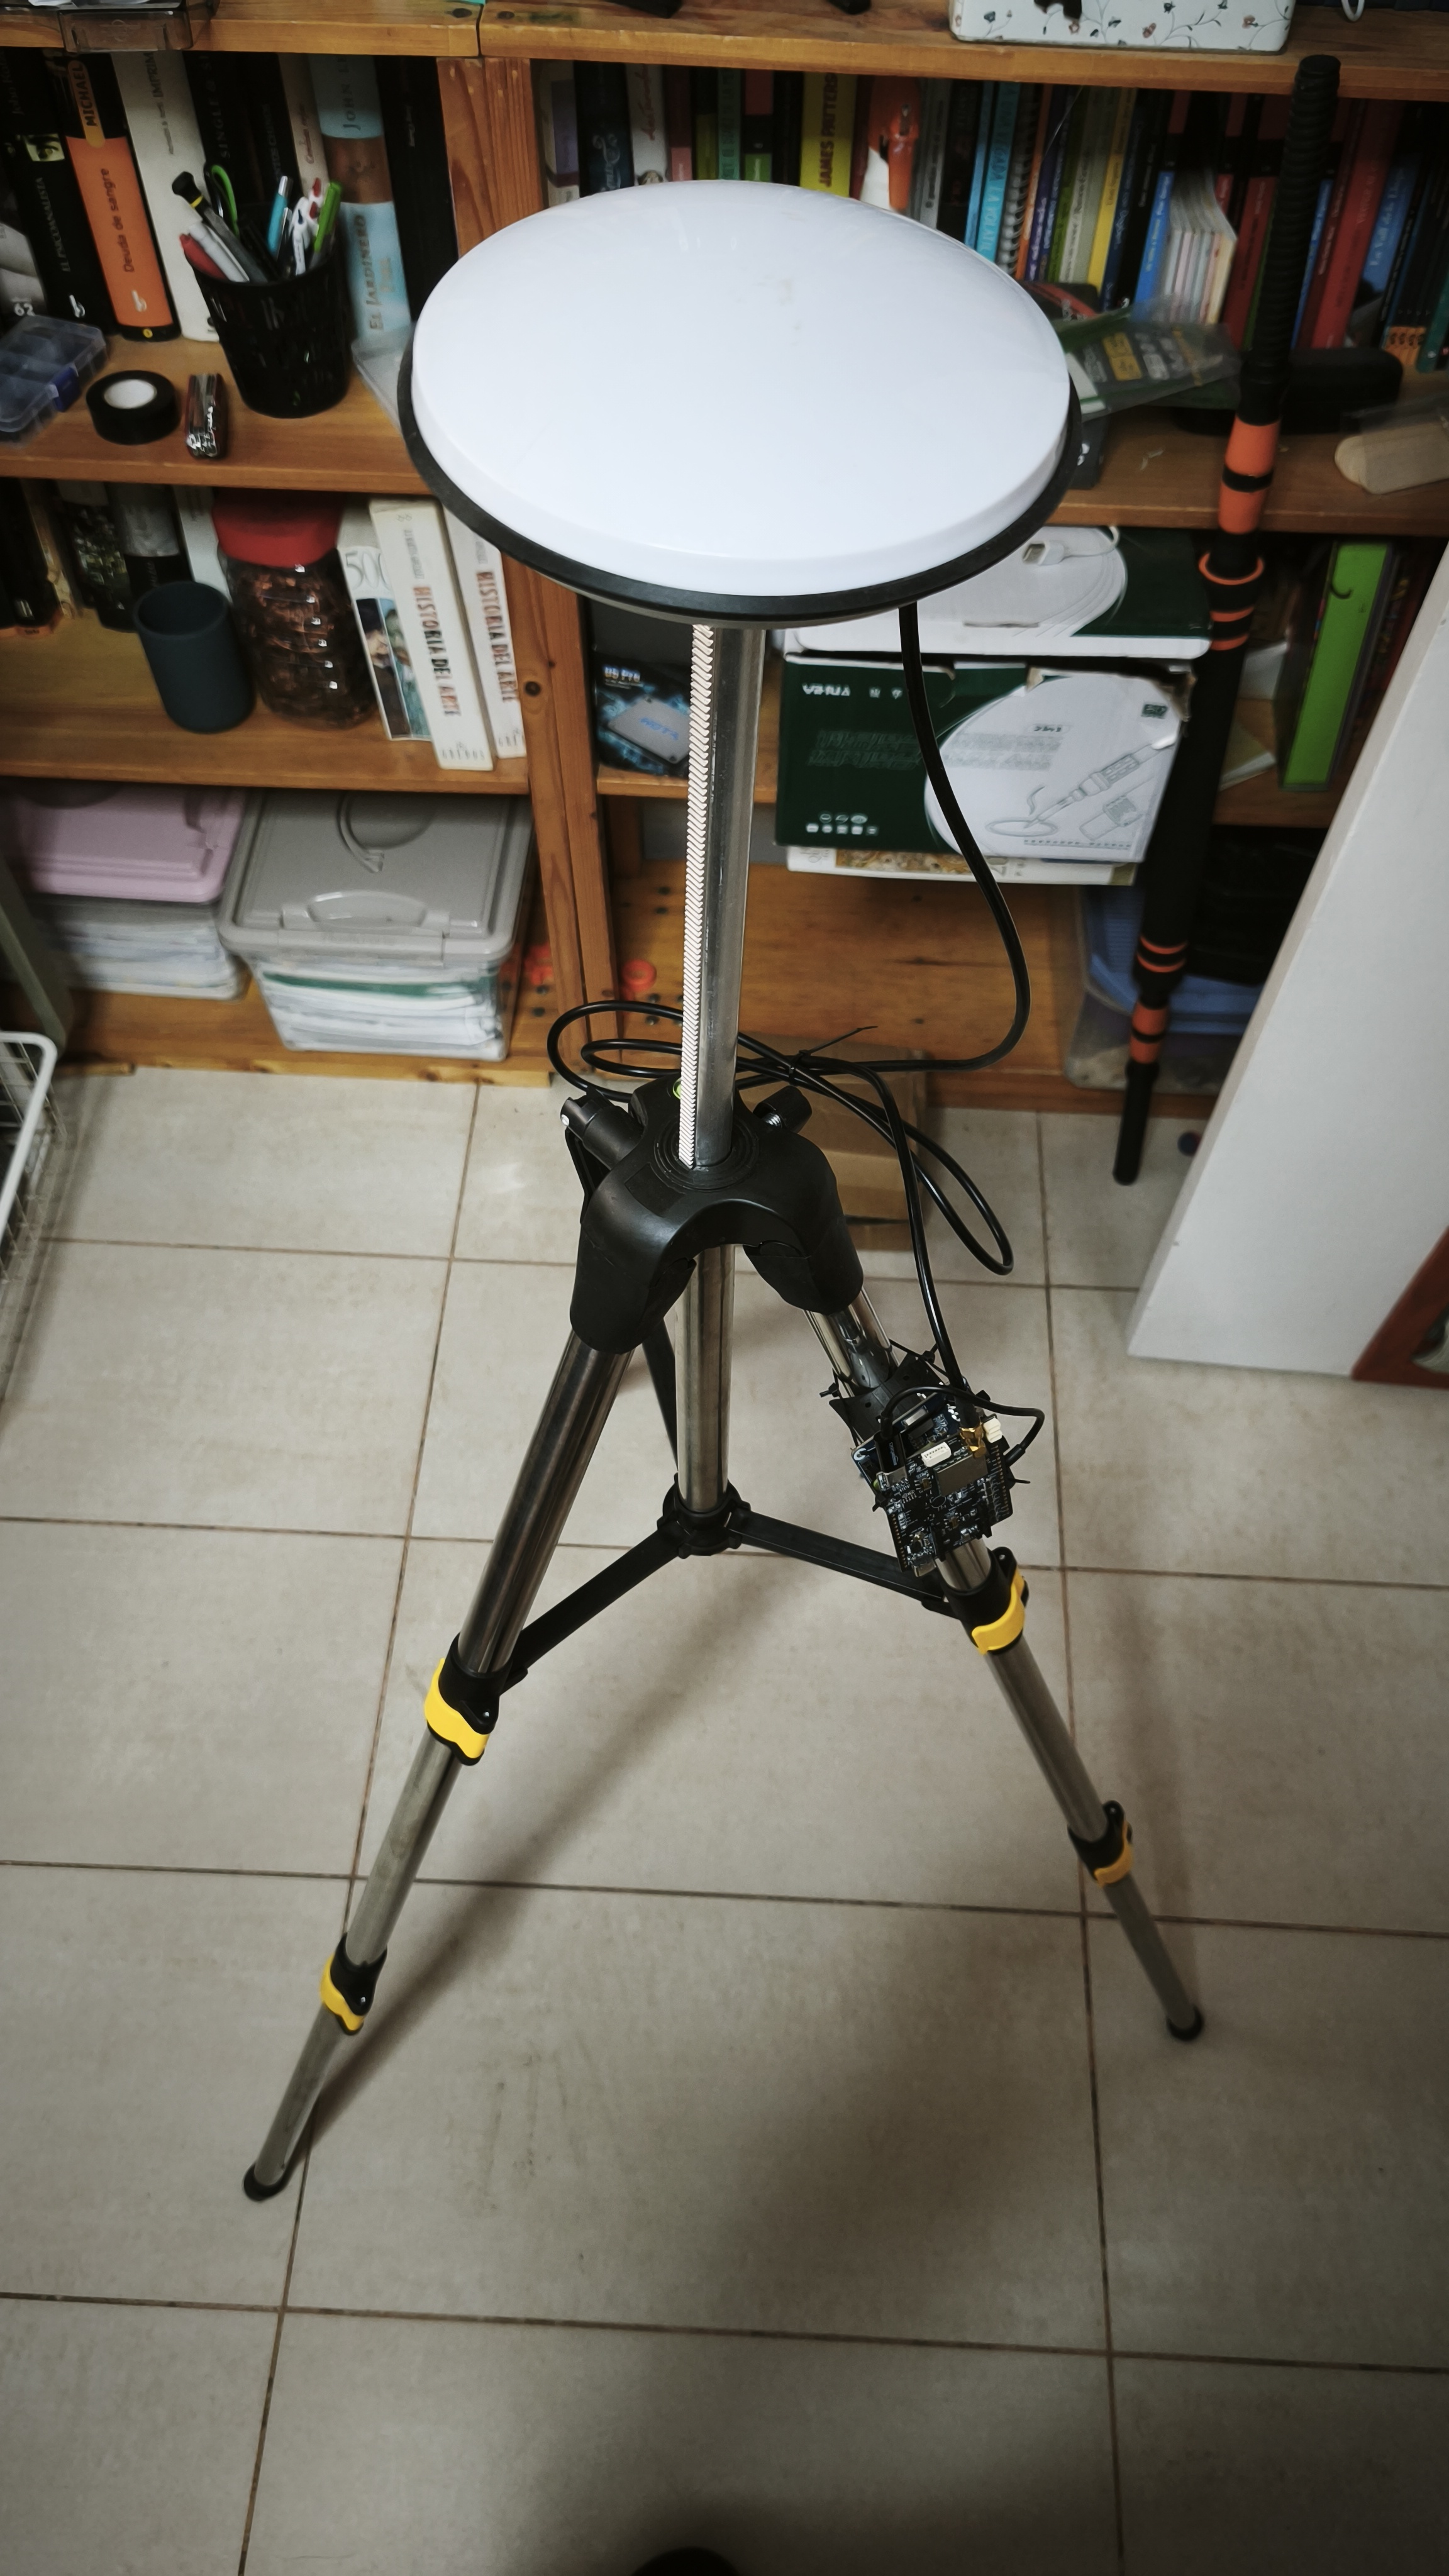
\includegraphics[width=\textwidth]{img/Base_sencera.jpg}
        \caption{Base completa sobre el trípode.}
    \end{subfigure}
    \hfill
    \begin{subfigure}[b]{0.43\textwidth}
        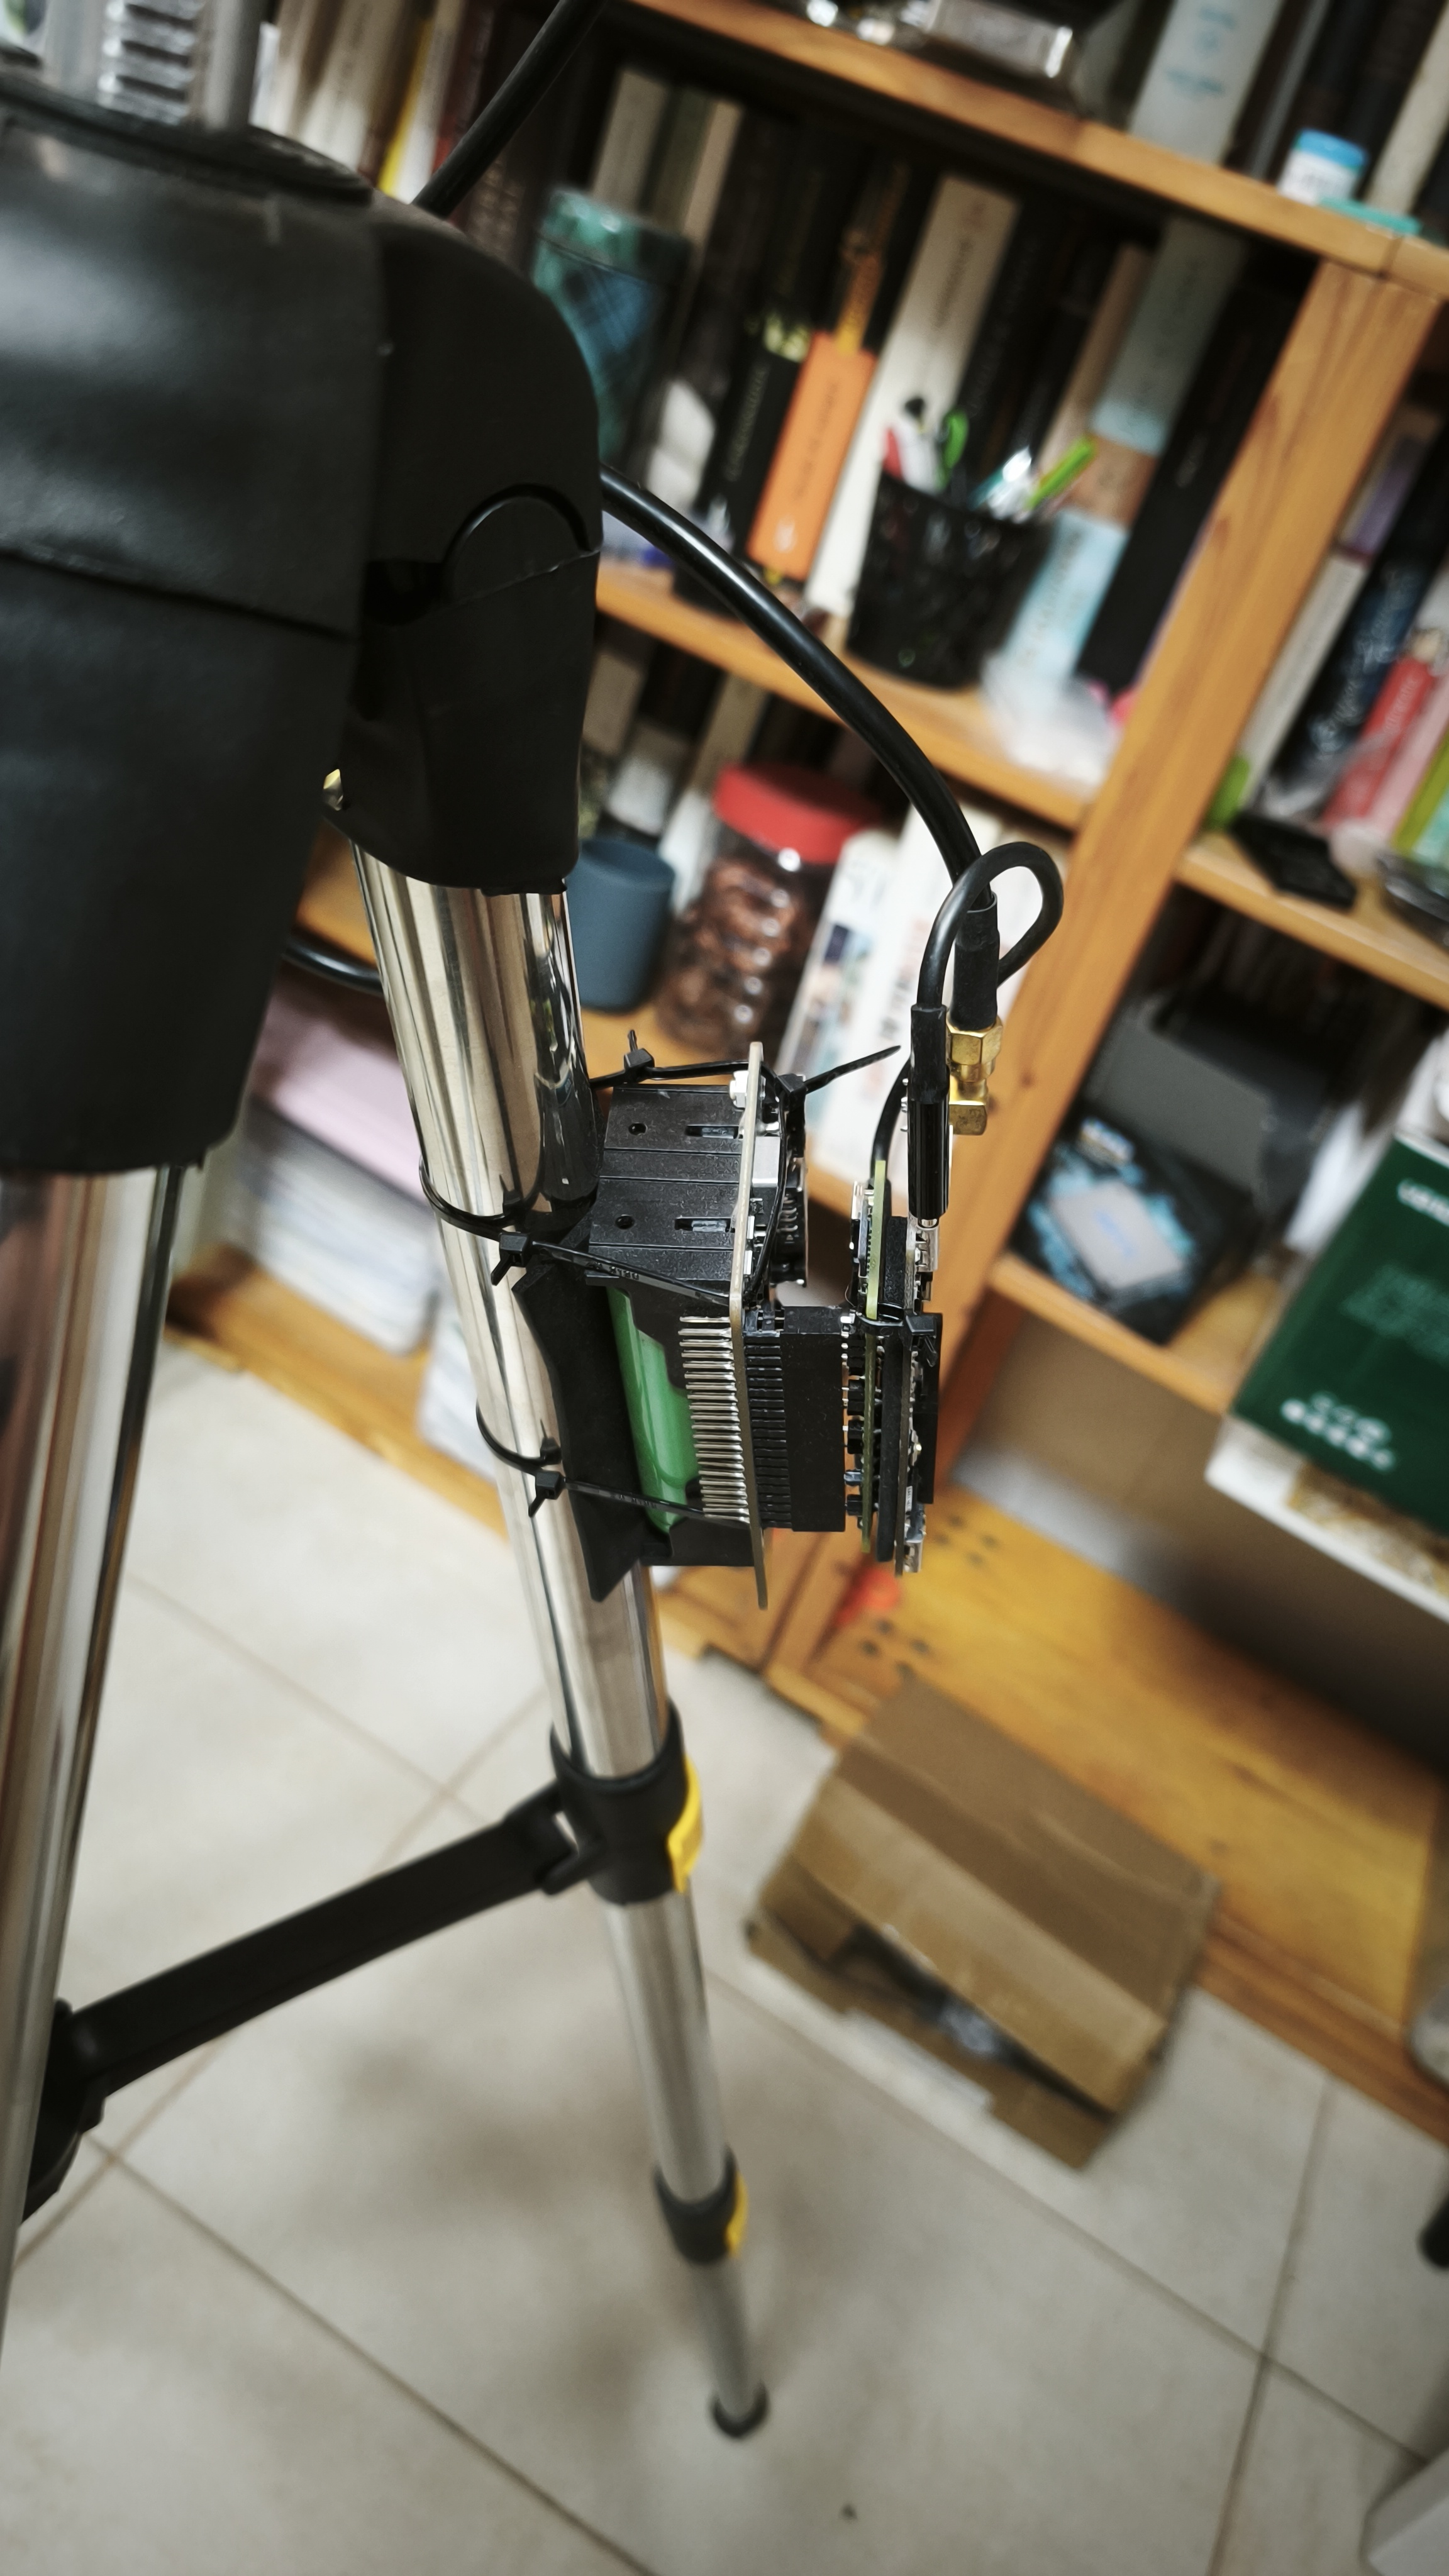
\includegraphics[width=\textwidth]{img/Stack_base.jpg}
        \caption{Pila de la base fixada a una pota.}
    \end{subfigure}
    \caption{Base RTK: antena multibanda sobre el trípode i pila amb el simpleRTK2B Pro, la Raspberry Pi i el UPS HAT.}
    \label{fig:base}
\end{figure}

El procediment de posicionament i de fixació de les coordenades de la base es descriu a \cref{sec:protocol-camp}.

\paragraph{Programari i configuració.} La Raspberry Pi funciona amb Raspberry Pi OS (Debian~13, 32~bits). Les correccions les distribueix el programa \texttt{str2str} de RTKLIB (la còpia \texttt{rtklibexplorer}, compilada a la pròpia Pi), executat com a servei \texttt{systemd} que arrenca amb la placa. El servei es diu \texttt{rtkbase}, però no té relació amb el projecte \texttt{rtkbase} de la bibliografia: llegeix el port sèrie USB del receptor (115\,200~bd) i obre un servidor TCP al port 5000 que reenvia el flux del receptor tal com surt (RTCM3 i els missatges UBX de navegació que emet pel mateix port), sense NTRIP. A més de reenviar-lo, el servei el desa a un fitxer durant tota la sessió (\cref{sec:protocol-camp}). La GS s'hi connecta amb \emph{RTK/GPS Inject} de Mission Planner en mode \emph{TCP Client}, a \texttt{192.168.4.1:5000}.

El punt d'accés WiFi (\texttt{BaseRTK}) el gestiona NetworkManager en mode \emph{shared}: banda de 2,4~GHz, canal~6, WPA-PSK, adreça \texttt{192.168.4.1/24} amb DHCP, i s'activa a cada arrencada. Cal desactivar el PMF (802.11w), perquè el controlador \texttt{brcmfmac} de la Pi no el suporta en mode AP.

El ZED-F9P (\emph{firmware} HPG~1.51, protocol~27.50) es configura amb \texttt{ubxtool}: NMEA desactivat al port USB, RTCM3 activat i els missatges 1005, 1074, 1084, 1094, 1124 i 1230 a 1~Hz. El flux total del port 5000, amb els missatges UBX de navegació que el receptor també emet, va ser d'uns 15~kbps. La posició de la base no es fixa: el receptor fa un \emph{survey-in} a cada sessió, amb 300~s com a mínim i fins que la precisió de la mitjana és de 2~m o millor, i la configuració queda guardada a la memòria \emph{flash} del receptor. Els vols de prova 5 i 6 van fer servir aquesta base i aquest mètode, amb l'antena a 122~cm.

\textbf{Limitació.} Als vols de prova 5 i 6 el servei només reenviava el flux, sense desar-lo, i no es va anotar la posició resultant del \emph{survey-in}; per això la posició absoluta d'aquells vols no es pot recuperar. Com que cada sessió en fa un de nou, la posició absoluta del mapa té un error comú de l'ordre de metres; això desplaça el mapa sencer però no en canvia la geometria relativa. Des del 27 d'octubre de 2026 el servei desa el flux de cada sessió, de manera que la posició es pot calcular a posteriori (\cref{sec:protocol-camp}).

\section{Estat del sistema}
\label{sec:estat-actual}

El maquinari està complet i el sistema ha acumulat uns 30~minuts de vol segons el comptador del controlador, repartits entre la campanya de posada a punt (\cref{chap:proves-vol}) i dos vols de fotogrametria (\cref{chap:vols-prova}). Amb la configuració actual el dron vola amb RTK Fixed als dos receptors i \emph{yaw} GNSS vàlid, i la cadena fotogràfica (dispar per distància, \emph{feedback} de la sabata, geoetiquetat i processat) està operativa de punta a punta. Les limitacions vigents --~sobretot l'autonomia i la validació absoluta amb punts de control~-- es recullen a \cref{sec:balanc-vols,sec:autonomia}, i el treball pendent és a \cref{sec:pendents-proves-vol}.

\chapter{Manual d'operació i procediments}
\label{chap:manual}

Aquest capítol recull la configuració de referència del sistema i el procediment de treball, aplicables a qualsevol vol de fotogrametria. Els resultats obtinguts amb aquests procediments es presenten al \cref{chap:vols-prova}.

\section{Antenes GNSS}
\label{sec:antenes-gnss}

\subsection{Antenes helicals del dron}

Les dues antenes helicals del \emph{rover} van muntades:
\begin{itemize}
    \item Verticals, paral·leles entre elles, apuntant amunt.
    \item Al punt més alt del dron.
    \item Amb una separació mínima de 10~cm respecte al VTx, els ESC i els cables de potència, per evitar interferències.
    \item Sense inclinació respecte a l'eix vertical.
\end{itemize}

\subsection{\emph{Baseline} del \emph{moving baseline}}

La separació entre les dues antenes helicals és de \textbf{0,38~m}, sobre un \emph{bracket} rígid de carboni alineat amb l'eix Y (lateral) del dron. Els \emph{offsets} respecte al centre de gravetat són $Y = \mp 0{,}19$~m i $Z = -0{,}10$~m (GPS1 a l'esquerra, GPS2 a la dreta), amb $X = 0$ (\cref{tab:params-gps-mb}).

La precisió de \emph{heading} d'un \emph{moving baseline} escala de manera inversament proporcional a la longitud del \emph{baseline}: amb 0,38~m s'estima una $\sigma$ de l'ordre de $0{,}5^{\circ}$, que cal validar de manera empírica (\cref{sec:validacio}). Qualsevol canvi en la longitud del \emph{bracket} requereix recalibrar el \emph{heading} GNSS.

\subsection{Antena de la base}

Antena de tipus \emph{patch} horitzontal amb pla de massa (\emph{ground plane}), anivellada sobre el trípode topogràfic.

\subsection{Sincronisme de la càmera}

El pin central de la sabata (\emph{hot-shoe}) de la càmera és el senyal \textbf{X-sync}: el Seagull SYNC2 hi encaixa directament, ja que la Sony $\alpha$6000 disposa d'una \emph{Multi Interface Shoe} compatible amb l'estàndard ISO~518.

\section{Configuració de ports sèrie del FC (Kakute H7)}
\label{sec:ports-serie}

\begin{table}[H]
    \centering
    \caption{Assignació de ports sèrie del Kakute H7}
    \label{tab:ports-serie}
    \begin{tabular}{lllc}
        \toprule
        Port & Funció & Baud rate & Protocol \\
        \midrule
        SERIAL0 (USB) & MAVLink2 (configuració) & -- & -- \\
        SERIAL1 (UART1, port VTX) & RFD868x MAVLink & 57600 & 2 \\
        SERIAL2 (UART2) & Bluetooth intern (ocupat) & -- & Deshabilitat \\
        SERIAL3 (UART3) & F9P \#1 -- GPS1 (MB-Base) & 230400 & 5 \\
        SERIAL4 (UART4) & F9P \#2 -- GPS2 (MB-Rover) & 230400 & 5 \\
        SERIAL6 (UART6) & RC ELRS (CRSF) & 420000 & 23 \\
        SERIAL7 (UART7, port ESC) & Telemetria ESC & 115200 & 16 \\
        \bottomrule
    \end{tabular}
\end{table}

\section{Configuració de la càmera}
\label{sec:config-camera}

\subsection{Paràmetres del controlador}

A partir d'ArduPilot 4.5, els paràmetres de càmera tenen el prefix \texttt{CAM1\_*} per donar suport multicàmera; la documentació i els fòrums antics encara fan servir noms \texttt{CAM\_*}.

\begin{table}[H]
    \centering
    \caption{Paràmetres de càmera (ArduPilot 4.5 o superior)}
    \label{tab:params-camera}
    \begin{tabular}{lP{9.5cm}}
        \toprule
        Paràmetre & Valor / Funció \\
        \midrule
        \texttt{SERVO5\_FUNCTION} & 10 (\emph{CameraTrigger}, MAP2 al pad M5) \\
        \texttt{CAM1\_TYPE} & 1 (Servo) \\
        \texttt{CAM1\_DURATION} & 1.0 (en \textbf{segons}, no ms): el MAP2 en mode IS-T necessita ordres d'1~s \\
        \texttt{CAM1\_SERVO\_ON} & 1700 (mode IS-T) \\
        \texttt{CAM1\_SERVO\_OFF} & 1500 (dins el rang de repòs del MAP2, 1400--1600) \\
        \texttt{SERVO5\_TRIM} & 1500 \\
        \texttt{CAM1\_TRIGG\_DIST} & 0 a la configuració base; es fixa a cada missió (\cref{sec:planificacio-vol}) \\
        \texttt{SERVO6\_FUNCTION} & $-1$ (GPIO per al \emph{feedback} del SYNC2, pad M6) \\
        \texttt{CAM1\_FEEDBAK\_PIN} & 55 \\
        \texttt{CAM1\_FEEDBAK\_POL} & 1 \\
        \bottomrule
    \end{tabular}
\end{table}

El nom del paràmetre és \texttt{CAM1\_FEEDBAK\_PIN}, escrit \textbf{sense la ``C''} de \emph{feedback} (nomenclatura històrica d'ArduPilot). El pin 55 correspon al pad de \texttt{SERVO6} reassignat com a GPIO.

Amb un objectiu manual sense contactes electrònics, el MAP2 no ha de treballar en mode AF-T (pre-enfocament d'1~s inútil, que afegeix retard constant). El detall del diagnòstic és a \cref{subsec:problemes-camera}.

\subsection{Ajust de la càmera}
\label{subsec:ajust-camera}

\begin{table}[H]
    \centering
    \caption{Ajust de la Sony $\alpha$6000 per a fotogrametria}
    \label{tab:ajust-camera}
    \begin{tabular}{ll}
        \toprule
        Ajust & Valor \\
        \midrule
        Mode d'exposició & M (manual) \\
        Temps d'obturació & 1/1600~s \\
        Diafragma & f/5,6 (anell fixat amb cinta) \\
        Enfocament & Manual a infinit (els dos anells fixats amb cinta) \\
        ISO & Automàtic, amb sostre a 1600 \\
        Mode de dispar & \emph{Single shot}, JPEG Fine \\
        Obturador & Electrònic de primera cortina activat \\
        \emph{Release w/o Lens} & Activat (necessari amb objectiu sense contactes) \\
        \bottomrule
    \end{tabular}
\end{table}

L'òptica manual no transmet dades a la càmera: l'EXIF grava \texttt{FocalLength=0} i \texttt{LensModel} buit, i l'orientació dependria del rumb (\cref{sec:processament-fotos}). Aquestes metadades es reescriuen en el post-procés.

La càmera no té marge dinàmic per compensar la poca llum: les fotografies s'han de fer amb el sol a més de 10--15$^{\circ}$ sobre l'horitzó (\cref{sec:vol6}).

\subsection{Retard de l'obturador}

L'ordre de dispar del controlador (\texttt{TRIG}) i l'exposició real estan separats per $\approx 0{,}28$~s (\cref{sec:retard-obturador}); a 5~m/s són $\approx 1{,}4$~m. Per això el geoetiquetat fa servir la posició del missatge \texttt{CAM} (instant del \emph{feedback} de la sabata) quan està disponible, i es compensa amb $v\cdot\tau$ quan no ho està.

\section{Configuració GPS \emph{moving baseline} i \emph{yaw}}
\label{subsec:gps-moving-baseline}

\begin{table}[H]
    \centering
    \caption{Paràmetres de \emph{moving baseline} i GPS-for-yaw}
    \label{tab:params-gps-mb}
    \begin{tabular}{ll}
        \toprule
        Paràmetre & Valor \\
        \midrule
        \texttt{GPS1\_TYPE} & 17 (MB-Base) \\
        \texttt{GPS2\_TYPE} & 18 (MB-Rover) \\
        \texttt{GPS\_AUTO\_CONFIG} & 1 \\
        \texttt{GPS\_DRV\_OPTIONS} & 0 \\
        \texttt{GPS\_INJECT\_TO} & 127 \\
        \texttt{EK3\_SRC1\_POSXY} / \texttt{VELXY} & 3 (GPS) \\
        \texttt{EK3\_SRC1\_YAW} & 2 (GPS yaw) \\
        \texttt{COMPASS\_ENABLE} & 0 (sense brúixola) \\
        \texttt{GPS1\_POS\_X/Y/Z} & $0$ / $-0{,}19$ / $-0{,}10$~m \\
        \texttt{GPS2\_POS\_X/Y/Z} & $0$ / $+0{,}19$ / $-0{,}10$~m \\
        \texttt{GPS1\_MB\_OFS\_Y} & $-0{,}38$~m \\
        \bottomrule
    \end{tabular}
\end{table}

\texttt{GPS\_DRV\_OPTIONS} ha de ser 0: el valor 1 (ús de l'UART2 per al \emph{moving baseline}) assumeix un cable directe entre els UART2 dels dos F9P per transportar el flux RTCM, que en aquest muntatge no existeix; amb el bit activat el \emph{rover} no arriba mai a RTK Fixed (\texttt{PreArm: GPS[2] yaw not available}). El flux entre receptors passa pel controlador de vol.

\section{Control, bateria i seguretat}
\label{sec:params-control}

\begin{table}[H]
    \centering
    \caption{Paràmetres de control, bateria i seguretat de la configuració de referència}
    \label{tab:params-control}
    \small
    \begin{tabular}{ll}
        \toprule
        Paràmetre & Valor \\
        \midrule
        \texttt{FRAME\_CLASS} & 1 (Quad) \\
        \texttt{FRAME\_TYPE} & 1 (X) \\
        \texttt{MOT\_PWM\_TYPE} & 5 (DShot300)~\cite{ardupilot_dshot} \\
        \texttt{ATC\_RAT\_RLL\_P} / \texttt{ATC\_RAT\_PIT\_P} & 0,07 \\
        \texttt{ATC\_RAT\_RLL\_I} / \texttt{ATC\_RAT\_PIT\_I} & 0,07 \\
        \texttt{ATC\_RAT\_RLL\_D} / \texttt{ATC\_RAT\_PIT\_D} & 0,002 \\
        \texttt{ATC\_RAT\_YAW\_P} & 0,10 \\
        \texttt{ATC\_RAT\_YAW\_I} & 0,01 \\
        \texttt{MOT\_THST\_EXPO} & 0,65 \\
        \texttt{MOT\_SPIN\_ARM} & 0,04 \\
        \texttt{MOT\_SPIN\_MIN} & 0,06 \\
        \texttt{MOT\_THST\_HOVER} & 0,225 (après en vol, \texttt{MOT\_HOVER\_LEARN=2}) \\
        \texttt{BATT\_MONITOR} & 4 (tensió i corrent analògics) \\
        \texttt{BATT\_VOLT\_MULT} & 10,82 (calibrat) \\
        \texttt{BATT\_AMP\_PERVLT} & 87,73 (calibrat) \\
        \texttt{BATT\_LOW\_VOLT} / \texttt{BATT\_FS\_LOW\_ACT} & 21,6~V / 2 (RTL) \\
        \texttt{BATT\_CRT\_VOLT} / \texttt{BATT\_FS\_CRT\_ACT} & 20,4~V / 1 (Land) \\
        \texttt{BATT\_FS\_VOLTSRC} & 0 (tensió instantània) \\
        \texttt{FENCE\_ENABLE} / \texttt{FENCE\_TYPE} & 1 / 7 (altura, cercle i polígon) \\
        \texttt{FENCE\_RADIUS} & 700~m \\
        \texttt{FENCE\_ALT\_MAX} & 120~m \\
        \texttt{WPNAV\_SPEED} & 500~cm/s (5~m/s) en missions automàtiques \\
        \texttt{FLTMODE1} a \texttt{FLTMODE6} & Stabilize, AltHold, Loiter, Auto, Guided, RTL \\
        \texttt{LOG\_BITMASK} & 196607 \\
        \bottomrule
    \end{tabular}
\end{table}

\section{Checklist pre-vol}
\label{sec:checklist-prevol}

\begin{enumerate}[label=\arabic*.]
    \item Verificar que els dos F9P (base i dron) reporten \texttt{RTK Fixed} abans d'armar, amb tipus de \emph{fix} correcte a tots dos receptors (no \texttt{RTK Float} ni \texttt{3D Fix}).
    \item Verificar que el \emph{yaw} GNSS (\emph{moving baseline}) és vàlid i coherent amb el \emph{heading} real (marge $< 1^{\circ}$).
    \item Comprovar l'enllaç RFD868x GS$\leftrightarrow$dron i la recepció de correccions RTCM al dron.
    \item Comprovar el nivell de bateria del dron (tensió per cel·la) i de la base (UPS).
    \item Comprovar la targeta SD i la bateria de la càmera, i que l'ajust és el de \cref{tab:ajust-camera}.
    \item Provar el disparador amb \emph{Trigger Camera Now} i confirmar que apareixen els missatges \texttt{CAM} (\emph{feedback} SYNC2 actiu).
    \item Revisar els modes de vol assignats i que el \emph{geofence} és actiu (\cref{tab:params-control}).
    \item Comprovar a Mission Planner que l'EKF3 és sa (sense advertiments de variància de posició o velocitat), que el HDOP és baix (recomanat $< 1$ amb RTK Fixed) i que no hi ha cap missatge de \emph{prearm} pendent.
    \item Verificar que \texttt{COMPASS\_ENABLE=0} i que no hi ha cap \emph{prearm error} de brúixola.
    \item Comprovar els \emph{failsafes}: pèrdua de RC, pèrdua de telemetria, bateria baixa i crítica.
    \item Comprovar que el sol és a més de 10--15$^{\circ}$ sobre l'horitzó i que l'àrea de vol i l'espai aeri ho permeten (\cref{sec:normativa}).
\end{enumerate}

\section{Planificació de vol}
\label{sec:planificacio-vol}

\subsection{Càlcul del GSD}

El \emph{Ground Sample Distance} depèn només de l'alçada de vol $H$, la mida del sensor, la distància focal $f$ i la resolució de la imatge:
\[
\mathrm{GSD}\,\text{(cm/px)} = \frac{H\,\text{(m)} \times \text{amplada del sensor (mm)} \times 100}{f\,\text{(mm)} \times \text{amplada de la imatge (px)}}
\]

Amb la Sony $\alpha$6000 (sensor APS-C de 23,5~$\times$~15,6~mm, 6000~$\times$~4000~px, mida de píxel $\approx 3{,}92$~\textmu m) i l'òptica TTArtisan de 25~mm:
\[
\mathrm{GSD}\,\text{(cm/px)} \approx 0{,}0157 \times H\,\text{(m)}
\]

\begin{table}[H]
    \centering
    \caption{GSD i cobertura per imatge segons l'alçada (Sony $\alpha$6000 + TTArtisan 25~mm)}
    \label{tab:gsd-altura}
    \begin{tabular}{ccc}
        \toprule
        Alçada (m) & GSD (cm/px) & Empremta (m, ample $\times$ alt) \\
        \midrule
        30 & 0,47 & 28,2 $\times$ 18,7 \\
        50 & 0,78 & 47,0 $\times$ 31,2 \\
        60 & 0,94 & 56,4 $\times$ 37,4 \\
        80 & 1,25 & 75,2 $\times$ 49,9 \\
        100 & 1,57 & 94,0 $\times$ 62,4 \\
        120 & 1,88 & 112,8 $\times$ 74,9 \\
        \bottomrule
    \end{tabular}
\end{table}

Els valors mesurats als vols de prova concorden amb aquesta relació: tenint en compte la focal calibrada pel processat (25,72~mm), un GSD de 0,451~cm/px correspon a 29,6~m d'alçada (vol previst a 30~m), i un GSD de 0,743~cm/px a 48,9~m (vol previst a $\sim$50~m).

\subsection{Paràmetres de vol}

\begin{table}[H]
    \centering
    \caption{Paràmetres de vol adoptats i recomanats}
    \label{tab:parametres-vol}
    \begin{tabular}{lP{9cm}}
        \toprule
        Paràmetre & Valor \\
        \midrule
        Alçada de vol & Segons el GSD objectiu (\cref{tab:gsd-altura}); 30~m i 50~m als vols de prova \\
        Solapament frontal / lateral & 75--77~\% / 65--69~\% al vol 5; 80~\% / 70~\% recomanat amb relleu complex \\
        Velocitat & 5~m/s (\texttt{WPNAV\_SPEED=500}); limitada pel \emph{motion blur}: $v_{\max} = \mathrm{GSD}/t_{\text{exposició}}$ \\
        Dispar & Per distància (\texttt{CAM1\_TRIGG\_DIST}), amb l'interval entre fotos superior a l'1~s de \texttt{CAM1\_DURATION} \\
        Orientació de la càmera & Costat llarg del sensor al llarg del sentit de vol \\
        Il·luminació & Sol a més de 10--15$^{\circ}$ sobre l'horitzó \\
        \bottomrule
    \end{tabular}
\end{table}

Els percentatges de solapament de 80/70~\% són el valor per defecte habitual en programari de fotogrametria per a projectes de precisió amb bona textura del terreny; es poden reduir amb precaució gràcies al geoetiquetat RTK, però un solapament insuficient continua limitant la qualitat del \emph{matching} SfM. Com que \texttt{CAM1\_DURATION=1.0} fixa un interval mínim d'aproximadament 1~s entre dispars, a 5~m/s la distància entre fotos ha de ser d'almenys 5~m (\cref{subsec:autonomia-altura}).

\section{Protocol de camp}
\label{sec:protocol-camp}

\subsection{Posicionar la base}
\begin{enumerate}[label=\alph*)]
    \item Trípode sobre un punt estable amb el cel net a 360$^{\circ}$, lluny de parets, cobertes metàl·liques i vehicles; mesurar l'alçada de l'antena (122~cm als vols de prova).
    \item Engegar la Pi i esperar uns 30~s que aparegui la xarxa \texttt{BaseRTK}; connectar-hi la GS.
    \item Reiniciar el \emph{survey-in} per esborrar la mitjana de la sessió anterior i esperar que sigui vàlid, des del PC connectat a \texttt{BaseRTK} i dins la carpeta \texttt{base\_rtk}: \texttt{python base\_rtk.py survey}. L'ordre va mostrant la durada, les observacions i l'error mitjà, i acaba quan el \emph{survey-in} és vàlid (mínim 300~s i error mitjà, \texttt{meanAcc}, de 2~m o millor) o als 20~min (\texttt{--minuts N} canvia el límit). Mentre dura, el servei \texttt{rtkbase} està aturat i el port 5000 no serveix; es reengega sol al final, també si es talla la connexió SSH o es prem Ctrl-C.
    \item Si no arriba a ser vàlid, la mitjana es queda estancada per \emph{multipath} o per obstrucció del cel: cal millorar la ubicació de l'antena, no allargar l'espera. El receptor continua amb el \emph{survey-in} en marxa, i \texttt{python base\_rtk.py survey --estat} el consulta sense reiniciar-lo.
    \item Quan el \emph{survey-in} és vàlid, l'ordre desa automàticament la posició ECEF (\texttt{meanX/Y/Z}) i la \texttt{meanAcc} finals a \texttt{survey.txt}, dins la sessió activa de la Pi. És l'únic registre de la posició de la base d'aquella sessió, i es baixa amb el registre (vegeu «Registre de la sessió» més avall).
\end{enumerate}

Mentre el \emph{survey-in} no és vàlid, el flux no porta el missatge 1005 (posició de la base) i el dron no pot arribar a RTK Fixed. La posició de la base és, doncs, la del \emph{survey-in}, amb un error de l'ordre de metres que desplaça tota la sessió (\cref{subsec:efecte-surveyin}). Per afirmar posicions absolutes caldrà reutilitzar una posició fixa registrada al mateix punt, o bé corregir el desplaçament de cada sessió amb una solució PPP del seu registre d'observacions.

\paragraph{Registre de la sessió.} El servei \texttt{rtkbase} desa el flux del receptor a fitxers mentre el reenvia pel port 5000, durant tota la sessió: \texttt{str2str} té dues sortides, \texttt{tcpsvr://:5000} i \texttt{file:///home/arnau/logs/actual/base\_\%Y\%m\%d\_\%h\%M.rtcm3::S=1}. Cada arrencada del servei obre una \emph{sessió} nova, una carpeta \texttt{/home/arnau/logs/sNNNN/} (\texttt{actual} apunta a la que està en curs), i dins s'hi crea un fitxer cada hora (\texttt{::S=1}). El nom dels fitxers porta l'hora UTC de la Pi, i la data és poc fiable, perquè la Pi no té rellotge de temps real ni internet: l'hora vàlida és la GNSS de dins de les dades. Un reinici del servei o un tall d'alimentació obre una sessió nova, tret del que fa \texttt{survey}, que continua a la mateixa. El registre és el mateix flux del port, uns 7~MB per hora, amb les observacions RTCM3 (pseudodistància, fase i C/N0 dels quatre sistemes), el missatge 1005 un cop el \emph{survey-in} és vàlid i els missatges UBX de navegació que el receptor emet pel mateix port. No porta efemèrides, que cal agafar d'una estació de referència propera, ni Doppler.

Al final de la sessió es baixa el registre abans d'apagar la base, des del PC connectat a \texttt{BaseRTK}, amb \texttt{python base\_rtk.py baixa} (la darrera sessió) o \texttt{python base\_rtk.py baixa N} (la sessió \texttt{N}; \texttt{python base\_rtk.py llista} mostra les que hi ha, amb mida i hores). L'ordre uneix els fitxers horaris de la sessió en un de sol, \texttt{base\_sNNNN.rtcm3}, en comprova la mida i, si hi ha notes del \emph{survey-in}, baixa també \texttt{base\_sNNNN\_survey.txt}. \texttt{-o carpeta} indica on es deixen, i no s'esborra res de la Pi. Es pot convertir el fitxer a RINEX amb \texttt{convbin -r rtcm3} per calcular a posteriori la posició de la sessió amb una solució PPP o relativa a una estació de referència. Aquest càlcul encara no s'ha fet amb cap registre.

Al disc de la Pi hi caben unes 3\,500~h de registre i no hi ha esborrat automàtic: les sessions que ja no calen s'esborren a mà amb \texttt{python base\_rtk.py esborra N} o \texttt{esborra --abans N}. L'ordre demana confirmació i no esborra mai la sessió activa. Les eines i la seva instal·lació són a la carpeta \texttt{base\_rtk}, amb el seu \texttt{README.md}.

\subsection{Verificar el \emph{moving baseline}}
\begin{enumerate}[label=\alph*)]
    \item Mesurar el vector real entre les dues antenes.
    \item Comprovar el \emph{yaw} GNSS contra el \emph{heading} real (marge $< 1^{\circ}$).
\end{enumerate}

\subsection{Vol}
\begin{enumerate}[label=\alph*)]
    \item Base en \texttt{Fixed} $\rightarrow$ la GS injecta RTCM al dron.
    \item Armar \textbf{només} amb RTK Fixed als dos F9P i \emph{yaw} vàlid.
    \item Volar el \emph{grid} planificat en mode Auto.
    \item Descarregar els \emph{logs} del FC (\texttt{.bin}) i les fotografies de la SD.
\end{enumerate}

\subsection{Post-procés}
\begin{enumerate}[label=\alph*)]
    \item Aparellar cada fotografia amb el seu missatge \texttt{CAM} (o \texttt{TRIG}) del \emph{log} i reescriure l'EXIF (\cref{sec:processament-fotos}).
    \item Generar el fitxer de geoetiquetes amb la precisió per foto.
    \item Processar amb ODX/WebODM (\cref{sec:processament}) i generar ortomosaic, DSM i núvol de punts.
\end{enumerate}

\section{Punts de control terrestre (GCP)}
\label{sec:gcp}

La precisió del producte final només es pot afirmar amb punts mesurats de manera independent. Com que la base fa un \emph{survey-in} a cada sessió, el \textbf{marc de coordenades} dels punts és tan important com la seva precisió. El protocol previst és:
\begin{itemize}
    \item Dianes ben distribuïdes per tota l'àrea, incloent-hi les cantonades i el centre, marcades amb un patró d'alt contrast reconeixible a la fotografia: com a mínim cinc de control i, a part, deu de comprovació (\cref{subsec:pla-precisio}).
    \item Posició de cada diana mesurada amb RTK contra \textbf{la mateixa base i la mateixa sessió} que el vol, amb una precisió prevista d'1--2~cm. Així els punts i els \emph{geotags} comparteixen el desplaçament del \emph{survey-in} i aquest s'anul·la a la comparació. Si es mesuren amb estació total o amb una altra base, cal ajustar-hi una transformació abans de comparar; si no, l'RMSE el domina l'error de metres de la base.
    \item Separar punts de control (que s'usen a l'ajust) de punts de comprovació (que no hi intervenen), i calcular l'RMSE H/V d'aquests últims.
\end{itemize}

\pendent{Encara no s'ha desplegat cap diana ni mesurat cap punt de control: aquest és el protocol previst, no un resultat. És la tasca que desbloqueja la precisió absoluta.}

\section{Processament (\emph{Structure from Motion} i PPK)}
\label{sec:processament}

El processament fotogramètric es fa amb el motor ODX 3.8.3 (WebODM 3.3.0, NodeODX 2.3.1) en un PC amb un i5-10400F, 32~GB de RAM i una RTX~2060. Un vol de 118 fotografies triga uns 42~minuts. Les opcions que s'aparten dels valors per defecte són: resolució d'ortofoto de 1~cm/px, resolució de DEM de 2~cm/px, qualitat del núvol de punts alta, generació de DSM, \emph{auto-boundary}, COG, glTF i \emph{point cloud} EPT. El detall de cada processat és a \cref{chap:vols-prova}.

Com a alternativa o complement al RTK en temps real, es contempla el post-procés \textbf{PPK} amb RTKLIB a partir dels enregistraments \texttt{UBX} en brut de la base i del dron, que dona una solució de posicionament independent de la qualitat de l'enllaç RTK durant el vol.

\pendent{El PPK no s'ha aplicat encara a cap vol: els processats actuals fan servir les posicions RTK en temps real del controlador.}

\section{Control de qualitat i criteris de validació}
\label{sec:validacio}

\subsection{Efecte del \emph{survey-in} sobre la validació}
\label{subsec:efecte-surveyin}

Amb el \emph{survey-in} la base calcula la seva posició com a mitjana de posicions autònomes, sense correccions, i la difon al missatge 1005. L'error d'aquesta posició es transmet íntegrament al \emph{rover}~\cite{ublox_f9p_im}: tota la sessió queda desplaçada pel mateix vector, que és de l'ordre de metres (el criteri d'acceptació del protocol és una \texttt{meanAcc} d'$\leq 2$~m). En canvi, la posició \emph{relativa} respecte a la base gairebé no es veu afectada: l'error de longitud de la línia de base és el de la base multiplicat per la línia de base i dividit per la distància als satèl·lits ($\sim 2\cdot 10^{7}$~m), uns 0,02~mm amb una base desplaçada 2~m i una línia de base de 200~m.

\begin{itemize}
    \item \textbf{No afectat} (es pot validar sense referència absoluta): l'exactitud de la línia de base RTK, la repetibilitat del \emph{rover}, el \emph{heading} i la geometria interna del producte (forma i escala).
    \item \textbf{Afectat:} la posició absoluta del mapa, la comparabilitat entre sessions i qualsevol comparació amb una referència externa. Com que cada sessió fa un \emph{survey-in} nou, dos mapes del mateix lloc queden desplaçats entre ells de l'ordre de metres. L'alçada de l'antena de la base (122~cm) entra a la cota amb pes 1:1.
\end{itemize}

Per recuperar la posició absoluta hi ha tres vies, no excloents: reutilitzar una posició fixa registrada al mateix punt; mesurar un punt conegut amb la mateixa base i corregir-ne el desplaçament; o calcular la posició de la sessió per PPP a partir del registre de la base i aplicar-ne el vector de correcció a tot el producte. Aquesta última és viable en principi amb el flux RTCM ja generat, que conté observacions MSM (1074, 1084, 1094, 1124) convertibles a RINEX amb RTKLIB (\texttt{convbin}); cal verificar-ho i que la sessió duri prou hores per a un PPP de nivell centimètric.

\subsection{Pla de proves de precisió}
\label{subsec:pla-precisio}

\begin{table}[H]
    \centering
    \caption{Pla de proves de precisió amb \emph{survey-in} i estat actual}
    \label{tab:validacio}
    \footnotesize
    \begin{tabular}{P{0.8cm}P{4.9cm}P{2.8cm}P{2.6cm}P{2.4cm}}
        \toprule
        Prova & Procediment & Marc de referència & Criteri & Estat \\
        \midrule
        T1 & Registrar \texttt{NAV-SVIN} (\texttt{meanX/Y/Z}, \texttt{meanAcc}) a cada sessió i, a mostres, comparar-lo amb la solució PPP del mateix lloc & --- & Informatiu: documenta el desplaçament & \textbf{Pendent}; no registrat als vols 5 i 6 \\
        T2 & \emph{Rover} estàtic a tres distàncies (p.~ex.\ 10, 50 i 100~m): vector base$\rightarrow$\emph{rover} RTK contra una mesura independent (estació total o distanciòmetre i nivell) & Relatiu a la base (independent del \emph{survey-in}) & $< 2$~cm H, $< 3$~cm V & \textbf{Pendent} \\
        T3 & Repetibilitat estàtica: 10--15~min sobre un punt; desviació estàndard H/V i percentatge de RTK Fixed & Relatiu & Coherent amb 0,01~m + 1~ppm & \textbf{Pendent} \\
        T4 & \emph{Heading}: \emph{yaw} GNSS contra un rumb de referència mesurat amb estació total, en diverses orientacions & Independent de la base & $\sigma < 0{,}5^{\circ}$ & \textbf{Pendent}; \emph{yaw} vàlid en tots els vols \\
        T5 & Producte fotogramètric: RMSE dels punts de comprovació, amb i sense punts de control, informant del nombre de punts & Mateix marc que els \emph{geotags} (mateixa base i sessió) & $< 3$~cm H, $< 5$~cm V & \textbf{Pendent}; consistència interna: reprojecció 0,90~px, model--GPS CE90 0,59~m \\
        T6 & Precisió absoluta: aplicar el vector PPP de la base i comprovar sobre una marca geodèsica coneguda & Marc extern (EPSG:32631) & Per definir (limitat pel PPP) & \textbf{Pendent}; requereix el registre de la base \\
        \bottomrule
    \end{tabular}
\end{table}

La comparativa amb un \emph{dataset} de referència DJI P4 RTK només té sentit després de T6, perquè necessita un mapa georeferenciat en absolut.

Sobre el nombre de punts: amb només cinc la incertesa de l'RMSE és gran. L'edició 2 de l'estàndard ASPRS demana un mínim de 30 punts de comprovació per afirmar una precisió de producte, i admet un nombre menor en projectes petits amb UAS si l'informe ho declara~\cite{asprs2023}. Per això es recomana un mínim de deu de comprovació, a més dels de control, i indicar-ne sempre el nombre.

Els indicadors de consistència interna (error de reprojecció, diferència entre el model i les posicions GPS de les fotos) mesuren la coherència del processat, \textbf{no la precisió}: no substitueixen T2--T6. Fins que no es facin, no s'afirma cap precisió absoluta ni centimètrica.

\section{Exportació de resultats}
\label{sec:exportacio}

Cada processat lliura, en el sistema de coordenades EPSG:32631 (UTM 31N), els productes següents: ortofoto GeoTIFF (1~cm/px a 30~m), DSM GeoTIFF (2~cm/px), núvol de punts dens (LAZ i EPT), models texturats (OBJ i GLB) i un informe PDF amb les estadístiques del processat.

\section{Manteniment del dron}
\label{sec:manteniment}

\subsection{Abans de cada vol}
\begin{itemize}
    \item Inspecció visual del \emph{frame}, els braços i els \emph{standoffs}: fissures o joc mecànic.
    \item Hèlixs sense esquerdes ni deformacions, equilibrades i amb els collarins ben apretats.
    \item Connectors XT60/XT90 i JST-GH sense joc ni signes d'escalfament.
    \item Antenes helicals ben fixades, verticals i sense danys al \emph{bracket} de \emph{baseline}.
    \item Estat de la bateria (inflor, tensió per cel·la) i càrrega suficient per al pla de vol.
    \item Targeta SD de la càmera amb espai lliure suficient i formatada correctament.
\end{itemize}

\subsection{Manteniment periòdic}
\begin{itemize}
    \item Revisió dels parells de collament de motors i braços cada poques sortides.
    \item Comprovació de l'estat dels coixinets dels motors (soroll, joc a l'eix).
    \item Actualització del \emph{firmware} d'ArduPilot i dels receptors F9P només de manera controlada, verificant la compatibilitat de paràmetres abans i després.
    \item Verificació periòdica del \emph{heading} GNSS contra una referència coneguda, per detectar deriva mecànica del \emph{bracket}.
    \item Neteja de contactes i connectors, especialment després de volar en ambients humits o amb pols.
    \item Cicles de manteniment de les bateries LiPo: emmagatzematge a tensió de repòs, sense descarregar per sota del llindar del fabricant, i retirada de qualsevol \emph{pack} que hagi patit un \emph{crash}.
\end{itemize}

\section{Normativa i seguretat}
\label{sec:normativa}

Aquesta secció és informativa i no constitueix assessorament legal. El marc normatiu EASA per a drones autoconstruïts està en transició; cal verificar-ne l'estat vigent abans de cada campanya de vol~\cite{easa_open_category}.

\subsection{Classificació del dron}

Aquest UAV és \textbf{autoconstruït} (\emph{privately built}): no prové d'un \emph{kit} llest per muntar comercialitzat com a producte únic, sinó de components individuals. Segons EASA, un dron autoconstruït \textbf{no pot portar marcat de classe C0--C4}, i per tant queda limitat, dins la categoria \emph{Open}, a la subcategoria \textbf{A3} (lluny de persones i de zones edificades), amb pes màxim de 25~kg~\cite{easa_open_category}.

Requisits pràctics derivats:
\begin{itemize}
    \item Registre com a operador de drones a l'autoritat aeronàutica competent (a l'Estat espanyol, AESA) i identificació visible del número de registre a l'aeronau.
    \item Certificat de pilot A1/A3 (formació en línia i examen) com a mínim; l'operador el té.
    \item Vol exclusivament en subcategoria A3: distància horitzontal mínima de 150~m respecte a zones residencials, comercials, industrials o recreatives, i lluny de persones alienes a l'operació.
    \item Comprovació de l'espai aeri i de les restriccions locals (zones \emph{geo-awareness}, NOTAM, proximitat a aeroports) abans de cada vol.
    \item Assegurança de responsabilitat civil, recomanable (obligatòria en molts casos segons el pes i l'ús).
\end{itemize}

Sota les regles transitòries, els drones autoconstruïts sense marcat de classe poden operar segons el règim heretat (per pes) fins a l'1 de gener de 2027. EASA desenvolupa un règim permanent per a drones autoconstruïts, equivalent aproximadament a la classe C4 (subcategoria A3, $<25$~kg, pilot amb certificat A1/A3)~\cite{easa_open_category}.

\subsection{Seguretat operacional}

\begin{itemize}
    \item No volar amb RTK Float ni sense \emph{fix} GNSS vàlid si la missió depèn de precisió centimètrica (a més, redueix la qualitat de l'estimació de posició de l'EKF3).
    \item Definir sempre un \emph{geofence} i accions de \emph{failsafe} per a bateria baixa i pèrdua d'enllaç.
    \item Mantenir contacte visual (VLOS) llevat que es disposi de l'autorització corresponent per a BVLOS.
    \item Avaluació de riscos bàsica de la zona de vol: obstacles, línies elèctriques, tercers i meteorologia (vent, pluja).
\end{itemize}

\section{Línies de continuïtat}
\label{sec:treball-futur}

\begin{itemize}
    \item Validació absoluta amb punts de control i de comprovació (\cref{sec:gcp}).
    \item Millora de l'autonomia: canvi del grup propulsor i bateria Li-ion (\cref{sec:autonomia,sec:propulsor}).
    \item Configuració del filtre \emph{notch} harmònic i Autotune.
    \item Migració a UM982: un sol mòdul amb \emph{heading} natiu, menys cablejat i menys consum.
    \item Integració de LiDAR (Livox Mid-360) per a vegetació densa.
    \item Càmera multiespectral per a agricultura de precisió.
    \item PCB \emph{carrier} pròpia (F9P + SBC + UPS integrats).
    \item Publicar correccions a una xarxa NTRIP comunitària (Centipède~\cite{centipede} o rtk2go).
\end{itemize}

\section{Projectes de referència}
\label{sec:referencies}

\begin{itemize}
    \item \texttt{rtkbase} (Stefal) -- programari de base~\cite{rtkbase}.
    \item SparkFun RTK Express -- disseny KiCad i \emph{firmware}~\cite{sparkfun_rtk_express}.
    \item \texttt{jacobjhansen/RTCM-Pi} -- flux de treball PPP~\cite{rtcm_pi}.
    \item Centipède -- xarxa NTRIP comunitària a Europa~\cite{centipede}.
    \item ArduPilot -- \emph{moving baseline} i GPS-for-yaw~\cite{ardupilot_moving_baseline}.
\end{itemize}


% =====================================================
% PART II — PROVES DE VOL
% =====================================================
\part{Proves de vol i posada a punt}
\chapter{Proves de vol i posada a punt}
\label{chap:proves-vol}

Aquest capítol recull la campanya de proves de vol i posada a punt feta entre agost i octubre de 2026, abans de l'operació en \emph{surveys} (\cref{chap:vols-prova}). Registra les incidències trobades en el control de vol, el GPS RTK, el mòdul de càmera i el grup propulsor, les causes identificades i els canvis aplicats per resoldre-les.

\begin{table}[H]
    \centering
    \caption{Sessions de vol de la campanya}
    \label{tab:sessions-vol}
    \small
    \begin{tabular}{llP{8.3cm}}
        \toprule
        Data & Sessió & Resultat \\
        \midrule
        6 d'agost & Posada a punt del control & Oscil·lació severa; \emph{crash} \\
        8 d'agost & Posada a punt del control & Dos vols correctes; \emph{crash} en canviar l'orientació \\
        10 d'agost & Prova GPS & Fallada d'un motor en vol; \emph{crash}; error de \emph{moving baseline} \\
        27 d'agost & Quatre vols & Quatre vols nets, RTK Fixed al 100~\% \\
        4 de setembre & Missió de \emph{grid} & Tallada pel \emph{geofence}; col·lapse de bateria \\
        8 d'octubre & Vol de prova 5 & 118 fotos; ortomosaic i DSM (\cref{sec:vol5}) \\
        13 d'octubre & Vol de prova 6 & Dos vols a l'alba; un lot aprofitable (\cref{sec:vol6}) \\
        20 d'octubre & Hèlixs de 8 polzades & Dos armats avortats (\cref{subsec:propulsor-8in}) \\
        \bottomrule
    \end{tabular}
\end{table}

\section{Configuració inicial del controlador}
\label{sec:config-inicial}

La primera revisió del fitxer de paràmetres del controlador va detectar i corregir els problemes següents:

\begin{itemize}
    \item \texttt{FRAME\_CLASS} sense assignar (ara Quad, X).
    \item \emph{Offsets} de posició dels GPS (\texttt{GPS1\_POS\_*} / \texttt{GPS2\_POS\_*}) a zero; mesurats respecte al centre de gravetat (\cref{tab:params-gps-mb}).
    \item \texttt{EK3\_SRC1\_YAW} apuntant a la brúixola: passat a GPS \emph{yaw}.
    \item Brúixola activada sense sensor connectat: desactivada.
    \item \texttt{BATT\_MONITOR} a 0: passat a tensió i corrent analògics.
    \item \texttt{MOT\_PWM\_TYPE} a PWM: passat a DShot300.
    \item Tots els modes de vol a Stabilize: assignats Stabilize, AltHold, Loiter, Auto, Guided i RTL.
    \item \texttt{SERVO9} assignat a \emph{Scripting1} sense ús real: desactivat.
\end{itemize}

\section{Cronologia d'incidents}
\label{sec:cronologia-incidents}

\subsection{6 d'agost -- Oscil·lació severa i \emph{crash}}

\emph{Wobbling} als braços en pujar gas, amb deriva lateral repetible. Al \emph{log}, el llaç de \emph{rate} canviava de signe al 65~\% de les mostres, amb errors de fins a $301^{\circ}$/s. Va acabar amb \texttt{Crash: Disarming: AngErr=51>30}.

Causes identificades:
\begin{itemize}
    \item Dron molt sobrepotenciat (\texttt{MOT\_THST\_HOVER=0{,}20}, \emph{hover} al 20~\%) amb PID de defecte pensats per a un \emph{hover} del 35--50~\%.
    \item Motors saturant al mínim per un \texttt{MOT\_SPIN\_MIN} massa alt.
    \item \texttt{MOT\_THST\_EXPO=0{,}8}.
    \item Sense filtre \emph{notch}, amb vibracions de 44~m/s\textsuperscript{2} i 42 \emph{clips}.
    \item Un \texttt{SAVE\_TRIM} fet en vol havia contaminat \texttt{AHRS\_TRIM\_X}.
\end{itemize}

\subsection{8 d'agost -- \emph{Crash} per canvi d'orientació}

Els dos primers vols del dia van anar bé (oscil·lació baixada del 65~\% al 3--6~\%, zero \emph{clips}). Al tercer, en posar \texttt{AHRS\_ORIENTATION} de 4 a 0, el dron va bolcar en 0,4~s amb el controlador saturat en sentit contrari al gir: realimentació positiva pura.

El problema real no era l'orientació sinó la polaritat del canal 2: el \emph{roll} responia correctament, només el \emph{pitch} estava invertit. Es va resoldre invertint l'\emph{elevator} al Radiomaster.

\subsection{10 d'agost -- \emph{Crash} per fallada de motor}

\emph{Hover} estable durant 10~s, després pèrdua sobtada. El motor M3 va quedar comandat a 2000 sense efecte; el corrent va baixar de 16~A a 8,9~A, el voltatge es va recuperar i les vibracions van caure just abans de la sortida: signatura inequívoca de motor aturat en vol.

El mateix dia es va identificar que \texttt{GPS\_DRV\_OPTIONS=1} impedia el \emph{moving baseline}: aquest valor assumeix un cable directe entre els UART2 dels dos F9P, que no existeix en aquest muntatge. El \emph{rover} no arribava mai a RTK Fixed, d'aquí el \texttt{PreArm: GPS[2] yaw not available} (\cref{subsec:gps-moving-baseline}).

\subsection{27 d'agost -- Quatre vols nets}

Primera sessió sense incidents. GPS[0] i GPS[1] al 100~\% de RTK Fixed, GPS \emph{yaw} disponible en totes les mostres, vibracions d'11--16~m/s\textsuperscript{2} i zero \emph{clips} als quatre vols.

\subsection{4 de setembre -- Missió tallada i \emph{crash} per bateria}

\textbf{Vol 1:} la missió es va avortar al \emph{waypoint} 25 de 87 per \emph{breach} del \emph{geofence}. El radi inicial de 300~m era insuficient per al camp nou (\emph{waypoint} més llunyà a 566~m; 41 dels 87 fora del radi). Les fotos van sortir borroses.

\textbf{Vol 2:} col·lapse de bateria. De 22,4~V a 8~V en 25~segons amb només 5~A de càrrega. El comptador marcava 213~mAh consumits d'un \emph{pack} de 4000, impossible: el sensor de corrent estava mal calibrat. El \emph{sag} va passar de 0,63~V a 1,79~V en 18~segons: resistència interna triplicada, una cel·la morint. Els \emph{failsafes} van actuar correctament (RTL a 758~s, Land a 763~s), però no hi havia energia per aterrar.

\subsection{4--13 de setembre -- Problemes de càmera}
\label{subsec:problemes-camera}

Al vol 1: 121 ordres de dispar, només 33 exposicions confirmades, totes amb un retard constant d'1,16~s. Al vol 2: 50 ordres, zero fotos.

Un primer diagnòstic va atribuir la lectura \texttt{FNumber=0}, \texttt{FocalLength=0} i \texttt{LensModel="----"} de l'EXIF a una fallada de contactes elèctrics. En realitat és el comportament normal d'un TTArtisan 25~mm f/2 manual, que no té contactes electrònics.

Causes reals:
\begin{itemize}
    \item El MAP2 estava en mode AF-T (\texttt{CAM1\_SERVO\_ON=1300}), que fa un pre-enfocament d'1~s inútil amb objectiu manual: d'aquí el retard constant.
    \item \texttt{CAM1\_SERVO\_OFF=1100} fora del rang de repòs que espera el MAP2 (1400--1600).
    \item \texttt{CAM1\_DURATION=0.1} massa curt perquè el MAP2 llegeixi el comandament (el mode IS-T vol 1,0~s).
    \item \emph{Release w/o Lens} possiblement desactivat, cosa que bloqueja el disparador amb un objectiu sense contactes.
    \item Obturació lenta i autofocus actiu al vol 1 (causa de les fotos borroses).
    \item La configuració del \emph{grid} assumia 20~mm quan l'objectiu real és de 25~mm: tot el solapament calculat era erroni.
\end{itemize}

Un cop aplicats els canvis, el vol 2 de la prova 6 va donar 110 ordres de dispar, 110 confirmacions de \emph{feedback} i 110 fotografies (\cref{sec:vol6}).

\section{Canvis de paràmetres aplicats}
\label{sec:canvis-aplicats}

\subsection{Control (6 d'agost)}

\begin{table}[H]
    \centering
    \caption{Ajust del control després de l'oscil·lació del 6 d'agost}
    \label{tab:canvis-control}
    \begin{tabular}{lll}
        \toprule
        Paràmetre & De & A \\
        \midrule
        \texttt{ATC\_RAT\_RLL\_P} / \texttt{PIT\_P} & 0,135 & 0,070 \\
        \texttt{ATC\_RAT\_RLL\_I} / \texttt{PIT\_I} & 0,135 & 0,070 \\
        \texttt{ATC\_RAT\_RLL\_D} / \texttt{PIT\_D} & 0,0036 & 0,0020 \\
        \texttt{ATC\_RAT\_YAW\_P} & 0,18 & 0,100 \\
        \texttt{MOT\_THST\_EXPO} & 0,8 & 0,65 \\
        \texttt{MOT\_SPIN\_ARM} & 0,10 & 0,04 \\
        \texttt{MOT\_SPIN\_MIN} & 0,15 & 0,06 \\
        \texttt{ATC\_RAT\_*\_FLTD} / \texttt{FLTT} & 20 & 10 \\
        \texttt{AHRS\_TRIM\_X} / \texttt{Y} & contaminats & recalibrats ($\approx 0$) \\
        \texttt{LOG\_BITMASK} & 180222 & 196607 \\
        \bottomrule
    \end{tabular}
\end{table}

\subsection{GPS}

\begin{table}[H]
    \centering
    \caption{Canvis de configuració GPS arran de la incidència del 10 d'agost}
    \label{tab:canvis-gps}
    \begin{tabular}{lll}
        \toprule
        Paràmetre & De & A \\
        \midrule
        \texttt{GPS\_DRV\_OPTIONS} & 1 & 0 \\
        \texttt{GPS1\_POS\_Y} / \texttt{GPS2\_POS\_Y} & 0 & $-0{,}19$ / $+0{,}19$ \\
        \texttt{GPS1\_POS\_Z} / \texttt{GPS2\_POS\_Z} & 0 & $-0{,}10$ / $-0{,}10$ \\
        \bottomrule
    \end{tabular}
\end{table}

\subsection{Seguretat i bateria}

\begin{table}[H]
    \centering
    \caption{Canvis de seguretat (\emph{failsafes}, \emph{geofence}) i de bateria arran del 4 de setembre}
    \label{tab:canvis-seguretat}
    \begin{tabular}{lll}
        \toprule
        Paràmetre & De & A \\
        \midrule
        \texttt{BATT\_FS\_LOW\_ACT} & 0 & 2 (RTL) \\
        \texttt{BATT\_FS\_CRT\_ACT} & 0 & 1 (Land) \\
        \texttt{BATT\_LOW\_VOLT} / \texttt{CRT\_VOLT} & -- & 21,6 / 20,4 \\
        \texttt{BATT\_AMP\_PERVLT} & sense calibrar & 87,73 \\
        \texttt{BATT\_VOLT\_MULT} & sense calibrar & 10,82 \\
        \texttt{FENCE\_ENABLE} & 0 & 1 \\
        \texttt{FENCE\_RADIUS} & 300 & 700 \\
        \texttt{WPNAV\_SPEED} & 1000 & 500 \\
        \texttt{SR1\_*} (telemetria RFD) & 0 & actius \\
        \bottomrule
    \end{tabular}
\end{table}

\subsection{Càmera}
\label{subsec:canvis-camera-pendents}

\begin{table}[H]
    \centering
    \caption{Canvis de càmera derivats del diagnòstic de \cref{subsec:problemes-camera}}
    \label{tab:canvis-camera}
    \begin{tabular}{lll}
        \toprule
        Paràmetre & Abans & Ara \\
        \midrule
        \texttt{CAM1\_SERVO\_ON} & 1300 (AF-T) & 1700 (IS-T) \\
        \texttt{CAM1\_SERVO\_OFF} & 1100 & 1500 \\
        \texttt{CAM1\_DURATION} & 0.1 & 1.0 \\
        \texttt{SERVO5\_TRIM} & 1100 & 1500 \\
        \bottomrule
    \end{tabular}
\end{table}

L'ajust físic de la càmera és a \cref{tab:ajust-camera}. El \emph{grid} de Mission Planner es planifica amb la focal real de 25~mm.

\section{Progressió mesurada}
\label{sec:progressio-mesurada}

\begin{table}[H]
    \centering
    \caption{Progressió de les mètriques de vol al llarg de la campanya}
    \label{tab:progressio}
    \begin{tabular}{lcccccc}
        \toprule
        Mètrica & 6 ago & 8 ago & 27 ago & 4 set & 8 oct & 13 oct \\
        \midrule
        Canvis de signe \emph{roll rate} & 65~\% & 3--6~\% & 8--9~\% & estable & -- & -- \\
        VibeZ màx.\ (m/s\textsuperscript{2}) & 44 & 40 & 11--16 & 14--18 & 10,8 & 14,1--15,7 \\
        \emph{Clips} & 42 & 0--29 & 0 & 0 & 0 & 0 \\
        GPS[0] RTK Fixed & -- & -- & 100~\% & 100~\% & 100~\% & -- \\
        GPS[1] RTK Fixed & -- & 0~\% & 100~\% & 100~\% & 100~\% & -- \\
        \emph{Hover throttle} & 20~\% & 20~\% & 45~\% & 45~\% & -- & -- \\
        \bottomrule
    \end{tabular}
\end{table}

Les columnes del 8 i del 13 d'octubre corresponen als vols de prova 5 i 6 (en el 6, el rang és el dels dos vols). La vibració s'ha calculat amb els missatges \texttt{VIBE} dels \emph{logs}, només amb els motors en marxa; la mediana de VibeZ és de 3,9~m/s\textsuperscript{2} al vol 5 i de 5,0--5,3~m/s\textsuperscript{2} al vol 6. Els guions són mètriques que no s'han calculat per a aquests vols.

\section{Autonomia i millora de rendiment}
\label{sec:autonomia}

L'autonomia és la limitació més gran de la plataforma actual. El \emph{hover} al 45~\% de \emph{throttle} (\cref{tab:progressio}) és estable, però el sistema carrega 520~g de càmera APS-C amb un grup propulsor que no es va escollir per eficiència (\cref{sec:propulsor}): funciona, però el preu és el temps de vol. Aquesta secció compara les opcions de millora per cost i guany esperat; el grup propulsor es detalla a la secció següent.

\begin{table}[H]
    \centering
    \caption{Opcions per millorar l'autonomia i el rendiment per bateria}
    \label{tab:opcions-autonomia}
    \small
    \begin{tabular}{P{3.4cm}P{1.7cm}P{2.5cm}P{5.9cm}}
        \toprule
        Opció & Cost & Guany & Comentari \\
        \midrule
        Volar a 45--50~m & 0~€ & $+60$~\% d'àrea per bateria & Cal recalcular el \emph{grid} amb la focal de 25~mm; també relaxa el ritme de dispar (\cref{subsec:autonomia-altura}). \\
        \emph{Notch} + Autotune & 0~€ & 5--10~\% & Veure \cref{subsec:autonomia-notch}. \\
        Bateria Li-ion 6S2P & $\sim$120~€ & $\times 1{,}7$ temps de vol & Molicel P42A o P45B. Evitar Samsung 50E: 10~A per cel·la és poc per a un \emph{hover} de $\sim$17~A (\cref{subsec:autonomia-liion}). \\
        Hèlixs de 8~polzades (motors actuals) & $\sim$15~€ & $+12$--$18$~\% d'autonomia & Aprofita el marge dels motors de 1100~KV (\cref{sec:propulsor}). \\
        Motors 400--500~KV + hèlixs de 12--13~polzades & $\sim$140~€ & $\sim\times 1{,}8$--$2$ temps de vol & El \emph{frame} de 500~mm actual ja ho permet; FC, F9P, ràdio i càmera es mantenen (\cref{subsec:autonomia-frame}). \\
        Li-ion + motors i hèlixs nous & $\sim$260~€ & 30+~min & El salt real a plataforma de \emph{survey}. \\
        \bottomrule
    \end{tabular}
\end{table}

\subsection{Pujar l'alçada de vol (cost zero)}
\label{subsec:autonomia-altura}

L'amplada de la franja fotografiada en cada passada és proporcional a l'alçada ($H \cdot 23{,}5/25$~m amb el sensor i l'òptica actuals, \cref{tab:gsd-altura}). Volant més alt es cobreix la mateixa àrea amb menys passades i, per tant, menys temps de vol: el guany és directament el quocient d'alçades. El vol de prova 5 es va fer a 30~m, de manera que pujar a 48~m dona el $+60$~\% d'àrea per bateria (45~m: $+50$~\%; 50~m: $+67$~\%), com ja es fa al vol de prova 6 (50~m).

El cost és GSD: a 50~m segueix sent $\approx 0{,}8$~cm/px, per sota del rang d'1--2~cm/px que es considera suficient per a topografia de precisió, de manera que hi ha marge per pujar sense perdre qualitat.

Pujar també relaxa el ritme de dispar. Amb un 80~\% de solapament frontal i un 70~\% de lateral, la distància entre fotos i entre línies creix amb l'alçada (suposant el costat curt del sensor al llarg de la ruta); a la velocitat actual de 5~m/s (\texttt{WPNAV\_SPEED=500}, \cref{tab:canvis-seguretat}), l'interval entre dispars és el de \cref{tab:ritme-dispar}.

\begin{table}[H]
    \centering
    \caption{Espaiat del \emph{grid} i interval de dispar segons l'alçada (25~mm, 80/70~\%, 5~m/s)}
    \label{tab:ritme-dispar}
    \small
    \begin{tabular}{ccccc}
        \toprule
        $H$ (m) & GSD (cm/px) & Entre fotos (m) & Entre línies (m) & Interval (s) \\
        \midrule
        30 & 0,47 & 3,7 & 8,5 & 0,75 \\
        40 & 0,63 & 5,0 & 11,3 & 1,00 \\
        45 & 0,71 & 5,6 & 12,7 & 1,12 \\
        50 & 0,78 & 6,2 & 14,1 & 1,25 \\
        \bottomrule
    \end{tabular}
\end{table}

El nou \texttt{CAM1\_DURATION=1.0} (\cref{tab:canvis-camera}) obliga a un interval mínim d'aproximadament 1~s entre ordres, de manera que a 40~m i 5~m/s ja s'està al límit, i a 30~m (0,75~s entre fotos) no seria viable amb aquests solapaments. A 45--50~m queda un petit marge, i a més es disparen menys fotos en total (menys dades a processar).

\subsection{\emph{Notch} i Autotune}
\label{subsec:autonomia-notch}

El filtre \emph{notch} harmònic (configurat a partir de la freqüència mesurada amb FFT en \emph{hover} i de les RPM de l'ESC) retira el soroll de vibració del llaç de control. Amb menys soroll, el controlador no ha de gastar autoritat en corregir-lo i els motors treballen més nets. L'Autotune, un cop el \emph{notch} està ben posat, permet apujar guanys sense reintroduir oscil·lació. El guany estimat és modest (5--10~\%), però no costa res.

\subsection{Bateria Li-ion 6S2P}
\label{subsec:autonomia-liion}

Un \emph{pack} 6S2P de cel·les 21700 de 4200~mAh (Molicel P42A) té $\approx 8{,}4$~Ah a $\approx 21{,}6$~V nominals, uns 181~Wh, davant els $\approx 89$~Wh del LiPo 6S 4000~mAh actual: més del doble d'energia. Com que el \emph{pack} també pesa més, el guany net de temps de vol s'estima en $\times 1{,}7$ i no $\times 2$.

L'elecció de la cel·la és crítica per la corrent. Segons la majoria de distribuïdors (xifres que cal contrastar amb el \emph{datasheet} del fabricant abans de comprar), la P42A (i la P45B) admet 45~A continus per cel·la, mentre que la Samsung 50E només 9,8~A. Amb un \emph{hover} de $\sim$17~A repartit en dues cel·les en paral·lel, cada cel·la porta $\sim$8,5~A: la 50E ja estaria al 87~\% del seu límit només volant estacionari, sense marge per maniobres ni per un \emph{sag} gran, mentre que la P42A treballa al 19~\%.

\subsection{Hèlixs grans i motors de KV baix}
\label{subsec:autonomia-frame}

És el factor dominant: l'eficiència d'un multirotor depèn de la càrrega de disc (empenta per unitat d'àrea escombrada), de manera que hèlixs més grans redueixen de forma directa la potència necessària en \emph{hover}. El \emph{frame} actual, de 500~mm entre eixos, ja admet hèlixs de fins a 13~polzades, però els motors de 1100~KV no hi són compatibles: el canvi té dos nivells (hèlixs de 8~polzades amb els motors actuals, o 12--13~polzades amb motors de 400--500~KV). La derivació, les compatibilitats KV--hèlix i el protocol de mesura es desenvolupen a \cref{sec:propulsor}. L'electrònica (FC, els dos F9P, la ràdio i la càmera) es manté sense canvis.

\section{Optimització del grup propulsor}
\label{sec:propulsor}

\subsection{Punt de partida i condicionant inicial}
\label{subsec:propulsor-inicial}

La configuració propulsora inicial del prototip va ser:

\begin{table}[H]
    \centering
    \caption{Configuració propulsora inicial}
    \label{tab:propulsor-inicial}
    \begin{tabular}{ll}
        \toprule
        Element & Especificació \\
        \midrule
        \emph{Frame} & Quad X, 500~mm entre eixos \\
        Motors & Pilotix 2808, 1100~KV \\
        Hèlixs & HQProp 7 $\times$ 4 $\times$ 3 (tripala) \\
        Bateria & LiPo 6S 4000~mAh \\
        AUW & 2,2~kg (inclosa la càrrega útil fotogràfica) \\
        \bottomrule
    \end{tabular}
\end{table}

L'elecció de les hèlixs de 7~polzades \textbf{no va respondre a un criteri de disseny sinó de disponibilitat}: eren hèlixs procedents d'un muntatge anterior i es van aprofitar per posar el prototip en vol sense cost addicional. Aquesta decisió va ser raonable en fase de posada en marxa --~el que calia validar aleshores era l'arquitectura RTK, el \emph{moving baseline} i la cadena de disparament de la càmera, no l'eficiència~-- però va quedar com a deute tècnic un cop el sistema va ser operatiu. La revisió posterior del grup propulsor és l'objecte d'aquesta secció.

\subsection{Diagnòstic}
\label{subsec:propulsor-diagnostic}

L'anàlisi dels registres de vol i de la geometria del \emph{frame} va revelar dues inconsistències.

\textbf{El \emph{frame} està infrautilitzat.} En una configuració en X, la distància entre motors adjacents és la diagonal dividida per $\sqrt{2}$:
\[
d_{\text{adjacent}} = \frac{500}{\sqrt{2}} \approx 354~\text{mm}
\]
Això permet hèlixs de fins a $\sim$330~mm (13~polzades) sense solapament entre discs. Amb hèlixs de 7~polzades (178~mm) s'estava aprofitant \textbf{només un 30~\% de l'àrea de disc disponible}.

\textbf{La relació empenta/pes és excessiva per a una plataforma de cartografia.} El paràmetre \texttt{MOT\_THST\_HOVER}, après en vol, és de 0,23: el \emph{hover} es manté amb una fracció baixa de l'empenta disponible. La relació empenta/pes resultant és de $\sim$3,1:1 quan per a una plataforma de cartografia n'hi ha prou amb 2:1. Un grup propulsor sobredimensionat en empenta i infradimensionat en àrea de disc treballa lluny del seu punt d'eficiència màxima.

Tots dos símptomes apunten al mateix: \textbf{el diàmetre de l'hèlix és el factor limitant}.

\subsection{Fonament teòric}
\label{subsec:propulsor-teoria}

La potència induïda que un rotor necessita per sostenir una empenta $T$ en estacionari ve donada per la teoria de quantitat de moviment:
\[
P_i = T \sqrt{\frac{T}{2\rho A}}, \qquad A = \frac{\pi D^2}{4}
\]
on $\rho$ és la densitat de l'aire i $A$ l'àrea de disc. Com que $P_i \propto 1/\sqrt{A} \propto 1/D$, \textbf{augmentar el diàmetre redueix la potència necessària de manera directa}. La magnitud rellevant és la càrrega de disc $T/A$: com més baixa, més eficient és el rotor.

Aplicat al cas ($T = 550$~g per motor, $\rho = 1{,}225$~kg/m\textsuperscript{3}):

\begin{table}[H]
    \centering
    \caption{Potència induïda ideal en \emph{hover} segons el diàmetre de l'hèlix}
    \label{tab:potencia-induida}
    \small
    \begin{tabular}{lcccc}
        \toprule
        Hèlix & Àrea de disc & Càrrega de disc & $P_i$ per motor & $P_i$ total \\
        \midrule
        7 polzades & 248~cm\textsuperscript{2} & 22,2~kg/m\textsuperscript{2} & 50,8~W & 203~W \\
        \textbf{8 polzades} & \textbf{324~cm\textsuperscript{2}} & \textbf{17,0~kg/m\textsuperscript{2}} & \textbf{44,5~W} & \textbf{178~W} \\
        13 polzades & 857~cm\textsuperscript{2} & 6,4~kg/m\textsuperscript{2} & 27,4~W & 109~W \\
        \bottomrule
    \end{tabular}
\end{table}

El pas de 7 a 8~polzades redueix la potència induïda ideal un \textbf{12,4~\%}; el pas a 13~polzades, un \textbf{46~\%}.

Aquests valors són el límit teòric: la potència real inclou la resistència de perfil de les pales (factor de mèrit típic 0,65--0,75) i el rendiment del conjunt motor-ESC. A la pràctica el guany total s'aproxima al de la component induïda, que és dominant en estacionari.

\subsection{Restricció de compatibilitat motor--hèlix}
\label{subsec:propulsor-kv}

L'àrea de disc no es pot augmentar lliurement: el KV del motor ha de correspondre al diàmetre de l'hèlix. Un motor amb KV massa alt per a la seva hèlix treballa a parell elevat i poques revolucions, lluny del seu punt de màxim rendiment, i el guany aerodinàmic es perd en pèrdues elèctriques i tèrmiques.

\begin{table}[H]
    \centering
    \caption{KV adequat segons el diàmetre de l'hèlix (tensió 6S)}
    \label{tab:kv-compatibilitat}
    \begin{tabular}{lcc}
        \toprule
        Hèlix & KV adequat & Motor actual (1100~KV) \\
        \midrule
        7 polzades & 1200--1400 & lleugerament baix \\
        \textbf{8 polzades} & \textbf{950--1100} & \textbf{correspondència òptima} \\
        9 polzades & 800--900 & $\sim$25~\% per sobre \\
        12--13 polzades & 400--500 & incompatible \\
        \bottomrule
    \end{tabular}
\end{table}

Aquesta restricció explica un resultat contraintuïtiu: \textbf{les hèlixs de 9~polzades rendirien pitjor que les de 8} malgrat tenir més àrea de disc, perquè el desajust de KV penalitza el motor més del que el disc aporta. Les de 8~polzades constitueixen, doncs, l'òptim assolible \textbf{sense substituir els motors}.

\subsection{Selecció de l'hèlix}
\label{subsec:propulsor-seleccio}

Un cop fixat el diàmetre, es van avaluar les opcions disponibles.

\textbf{Nombre de pales.} A igualtat de diàmetre i empenta, una hèlix bipala és aerodinàmicament més eficient que una tripala. Tanmateix, l'oferta de 8~polzades per a multirotor és majoritàriament tripala, i les bipales disponibles (APC 8$\times$4.5MR i MRP) tenen un \textbf{límit de règim de $\sim$13\,100~min\textsuperscript{$-1$}}. Amb 1100~KV sobre 6S (24\,400~min\textsuperscript{$-1$} en buit) aquest límit es podria superar en maniobres a gas ple --~ràfegues, recuperacions, pujades de \emph{failsafe}~--, amb risc de trencament de pala. Amb una càrrega útil fotogràfica al dessota, el criteri de fiabilitat preval sobre el guany marginal d'eficiència.

\textbf{Decisió:} es manté la configuració tripala i s'adopta una hèlix de \textbf{niló reforçat amb fibra de vidre}, dimensionada per als règims habituals en multirotors d'alta velocitat.

\begin{table}[H]
    \centering
    \caption{Hèlixs candidates de 8~polzades}
    \label{tab:helix-candidates}
    \small
    \begin{tabular}{llcP{6.4cm}}
        \toprule
        Candidata & Pas & Massa & Observacions \\
        \midrule
        \textbf{HQProp LR8X4.2X3} & 4,2 pol. & -- & Gamma \emph{Long Range}, dissenyada per a creuer eficient amb càrrega útil \\
        HQProp MacroQuad 8$\times$4$\times$3 & 4,0 pol. & 12,8~g & Boixa 15,7~mm, forat 9,5/5~mm (anells no inclosos) \\
        Gemfan 8040-3 & 4,0 pol. & -- & Equivalent, àmplia disponibilitat a Europa \\
        \bottomrule
    \end{tabular}
\end{table}

S'escull la \textbf{HQProp LR8X4.2X3}. La relació pas/diàmetre (0,53) és inferior a la de la configuració inicial (0,57), cosa que afavoreix el rendiment en estacionari i creuer lent, que és el règim de treball d'una missió de cartografia.

\subsection{Verificacions prèvies al muntatge}
\label{subsec:propulsor-verificacions}

\begin{itemize}
    \item \textbf{Diàmetre d'eix:} 5~mm, o anells adaptadors.
    \item \textbf{Camp de visió de la càmera:} el pas de 7 a 8~polzades afegeix 12,7~mm de radi per hèlix. Cal confirmar que les pales no entren al fotograma amb l'òptica de 25~mm en muntatge nadir.
    \item \textbf{Distància al terra} amb el tren d'aterratge actual.
    \item \textbf{Marge de corrent de l'ESC:} el corrent per motor disminueix en augmentar el diàmetre, de manera que no cal revisar el dimensionament.
\end{itemize}

\subsection{Primera prova amb hèlixs de 8 polzades (20 d'octubre)}
\label{subsec:propulsor-8in}

La primera prova amb les hèlixs de 8~polzades va quedar en dos armats avortats. En tots dos, el patró va ser el mateix: mode Loiter, rampa d'enlairament amb sortida de motors del 43--55~\%, 25--31~A, tensió superior a 23,85~V, i el \emph{log} s'acaba entre 0,1 i 0,5~s després, sense \emph{failsafe} ni error registrat.

El controlador es manté tranquil i els quatre motors són simètrics (dins del $\pm 2$~\%). La vibració, en canvi, és molt superior a la dels vols anteriors: 15--35~m/s\textsuperscript{2} al primer armat i 32--92~m/s\textsuperscript{2} (amb \emph{clipping}) al segon, davant d'una mediana de 3--5~m/s\textsuperscript{2} i un màxim de $\sim$16~m/s\textsuperscript{2} als vols previs. L'IMU en brut mostra una vibració tonal --~pics estrets a la freqüència de rotació, que creixen amb l'acceleració (127--134~Hz $\rightarrow$ 159--173~Hz)~-- i no de banda ampla, cosa que apunta a desequilibri de l'hèlix (component 1$\times$) més que no pas a fregament. Els paràmetres i filtres no es van retocar per al canvi d'hèlix. La causa exacta del tall del \emph{log} no s'ha determinat; la hipòtesi de treball és el desequilibri de les hèlixs, que cal descartar balancejant-les abans de repetir la prova.

\subsection{Reajustament del control}
\label{subsec:propulsor-control}

El canvi de diàmetre modifica la inèrcia rotacional i l'autoritat de control, de manera que els guanys del llaç de velocitat angular deixen de ser vàlids. Després del muntatge cal:

\begin{enumerate}[label=\arabic*.]
    \item \textbf{Refer el filtre \emph{notch} harmònic.} La freqüència fonamental dels motors baixa en augmentar el diàmetre. Procediment: \texttt{INS\_RAW\_LOG\_OPT = 9}, vol de 60--90~s amb maniobres variades, anàlisi amb l'eina \emph{Filter Review} d'ArduPilot.
    \item \textbf{Reduir els guanys P i D} dels eixos de \emph{roll} i \emph{pitch} com a punt de partida conservador, i executar \textbf{Autotune} eix per eix un cop verificat que el vol és estable.
\end{enumerate}

\subsection{Protocol de mesura}
\label{subsec:propulsor-mesura}

Per quantificar el guany real s'estableix un protocol de comparació controlada. \textbf{Requisit previ: calibració del sensor de corrent i de tensió} (\texttt{BATT\_AMP\_PERVLT}, \texttt{BATT\_VOLT\_MULT}), sense la qual les mesures d'energia no són vàlides. Aquest requisit ja està complert (\cref{tab:canvis-seguretat}).

\textbf{Condicions idèntiques entre assaigs:} mateixa quadrícula, altura, velocitat de creuer, càrrega útil, massa de bateria i condicions de vent ($< 3$~m/s).

\textbf{Variables a registrar en cada assaig:}

\begin{table}[H]
    \centering
    \caption{Variables a registrar per assaig}
    \label{tab:variables-mesura}
    \begin{tabular}{ll}
        \toprule
        Variable & Origen \\
        \midrule
        Energia consumida (mAh) & \texttt{BAT.CurrTot} al registre \\
        Temps armat (s) & marques \texttt{ARMED} / \texttt{DISARMED} \\
        Consum mitjà (A) & \texttt{BAT.Curr} \\
        Potència mitjana (W) & \texttt{BAT.Curr} $\times$ \texttt{BAT.Volt} \\
        Eficiència (g/W) & AUW $\div$ potència mitjana \\
        \texttt{MOT\_THST\_HOVER} & paràmetre après en vol \\
        Superfície coberta (ha) & planificació de la missió \\
        \bottomrule
    \end{tabular}
\end{table}

\textbf{Mètriques derivades:} mAh per minut, \textbf{hectàrees per bateria} (la magnitud rellevant per a l'operador) i g/W (la magnitud rellevant per a l'enginyeria).

\begin{table}[H]
    \centering
    \caption{Comparació de grup propulsor: configuració inicial (mesurada al vol de prova 6, vol 2) i hèlixs de 8~polzades (pendent)}
    \label{tab:resultats-propulsor}
    \begin{tabular}{lccc}
        \toprule
        Mètrica & 7 $\times$ 4 $\times$ 3 (inicial) & 8 $\times$ 4,2 $\times$ 3 & Variació \\
        \midrule
        Energia fins al \emph{failsafe} (mAh) & 2\,012 & pendent & \\
        Temps fins al \emph{failsafe} (min) & 10,6 & pendent & \\
        Consum mitjà (A) & 22 & pendent & \\
        Potència mitjana (W) & $\approx 500$ & pendent & \\
        Eficiència (g/W) & $\approx 4{,}4$ & pendent & \\
        \texttt{MOT\_THST\_HOVER} & 0,23 & pendent & \\
        Hectàrees per bateria a 50~m & 3,1 & pendent & \\
        \bottomrule
    \end{tabular}
\end{table}

\noindent\textit{Estimació prèvia: $+12$--$18$~\% d'autonomia.}

\smallskip
\noindent Els valors de la columna inicial provenen del vol 2 del vol de prova 6 (\cref{sec:vol6}), mesurats amb el sensor de corrent ja calibrat. La potència és el producte del corrent mitjà per una tensió mitjana de $\sim$22,5~V. Els dos vols de la prova 6 acaben per \emph{failsafe} de bateria baixa quan només s'ha gastat el 47--50~\% de la capacitat nominal, per la caiguda de tensió sota càrrega (\cref{sec:vol6}): l'autonomia útil la limita la tensió, no l'energia.

\subsection{Línia de continuïtat}
\label{subsec:propulsor-continuitat}

La configuració de 8~polzades esgota el marge disponible amb els motors actuals. L'aprofitament complet del \emph{frame} de 500~mm requereix substituir el grup motor:

\begin{table}[H]
    \centering
    \caption{Configuracions de grup propulsor i autonomia estimada}
    \label{tab:continuitat-propulsor}
    \small
    \begin{tabular}{lccc}
        \toprule
        Configuració & Càrrega de disc & $P_i$ teòrica & Autonomia estimada \\
        \midrule
        7 polzades (inicial) & 22,2~kg/m\textsuperscript{2} & 203~W & 10--11~min \\
        8 polzades & 17,0~kg/m\textsuperscript{2} & 178~W & 12--13~min \\
        \textbf{12--13 polzades, motors 450--500~KV} & \textbf{6,4~kg/m\textsuperscript{2}} & \textbf{109~W} & \textbf{18--22~min} \\
        \bottomrule
    \end{tabular}
\end{table}

Candidats: Sunnysky X3108 480~KV o T-Motor MN3110 470~KV amb hèlixs 12 $\times$ 4 o 13 $\times$ 4,4. La relació empenta/pes resultant ($\sim$2,6:1) continua sent adequada per a operació de cartografia. Cal verificar el patró de fixació dels braços: els motors de la sèrie 28xx solen muntar amb patró 16 $\times$ 16~mm i els 31xx amb 19 $\times$ 19 o 25 $\times$ 25~mm.

Combinat amb un \emph{pack} \textbf{Li-ion 6S2P} de cel·les d'alta descàrrega (Molicel P42A o P45B, 206~Wh/kg enfront dels 143~Wh/kg del LiPo actual; \cref{subsec:autonomia-liion}), l'autonomia projectada supera els 30~minuts.

\subsection{Conclusió}

La configuració inicial de 7~polzades va ser una decisió d'aprofitament de material, adequada per a la fase de posada en marxa però subòptima un cop el sistema va entrar en operació. L'anàlisi posterior identifica el diàmetre d'hèlix com el factor limitant de l'eficiència i estableix dues millores de cost molt diferent:

\begin{itemize}
    \item \textbf{Canvi a hèlixs de 8~polzades} ($\sim$15~€): aprofita el marge que permeten els motors actuals.
    \item \textbf{Canvi de grup motor a 12--13~polzades} ($\sim$140~€): aprofita el \emph{frame} ja existent i gairebé dobla l'autonomia.
\end{itemize}

Cap de les dues requereix modificar l'arquitectura RTK, la cadena fotogràfica ni el programari de vol, que es mantenen íntegres.


\section{Estat i treball pendent}
\label{sec:pendents-proves-vol}

\subsection{Resolt durant la campanya}
\begin{itemize}
    \item Control estable i \emph{moving baseline} amb RTK Fixed al 100~\% als dos receptors. La vibració, mesurada al \emph{log} (missatge \texttt{VIBE}) amb els motors en marxa, té una mediana de 2--5~m/s\textsuperscript{2} i un màxim de 10,8~m/s\textsuperscript{2} al vol de prova 5 i de 18,7~m/s\textsuperscript{2} al 6, sense \emph{clipping} (\cref{tab:progressio}).
    \item Sensor de corrent i de tensió calibrats (\texttt{BATT\_AMP\_PERVLT}, \texttt{BATT\_VOLT\_MULT}); el sensor de corrent llegia per sota del valor real, cosa que va amagar el consum real fins al col·lapse de bateria del 4 de setembre.
    \item Cadena de disparament de la càmera operativa: dispar IS-T, \emph{feedback} de la sabata al pin 55 (110 de 110 exposicions confirmades al vol 2 de la prova 6) i \emph{grid} planificat amb la focal real de 25~mm.
    \item \emph{Baseline} lateral amb GPS1 a l'esquerra (\texttt{GPS1\_POS\_Y=$-0{,}19$}), amb \emph{yaw} GNSS vàlid.
\end{itemize}

\subsection{Pendent: proves i millores}
\begin{itemize}
    \item \emph{Notch} harmònic: mesurar la freqüència amb FFT en \emph{hover} i configurar-lo en mode 3 (RPM d'ESC); l'\emph{IMU batch sampler} ja és actiu (\texttt{INS\_LOG\_BAT\_MASK=1}). Verificar \texttt{SERVO\_BLH\_POLES=14} contra el RPM real, perquè el \emph{notch} en depèn. Autotune a continuació.
    \item Bateria Li-ion 6S2P i, si cal més autonomia, canvi de grup motor (\cref{sec:autonomia}).
    \item Punts de control i de comprovació a terra, mesurats amb la mateixa base i sessió que el vol, per afirmar una precisió (\cref{sec:gcp}).
    \item Calcular per PPP el desplaçament de la primera sessió amb registre de la base (el servei ja desa el flux i la posició del \emph{survey-in} de cada sessió, \cref{sec:protocol-camp}) i comprovar que la conversió a RINEX funciona (\cref{subsec:efecte-surveyin}).
    \item Repetir el vol de camp (vol de prova 6) amb el sol a més de 10--15$^{\circ}$ (\cref{sec:vol6}).
    \item Pla de proves de precisió T1--T6 (\cref{tab:validacio}), amb el \emph{heading} GNSS i l'exactitud de la línia de base RTK; aplicació del PPK (\cref{sec:processament}).
\end{itemize}


% =====================================================
% PART III — VOLS DE FOTOGRAMETRIA
% =====================================================
\part{Resultats fotogramètrics}
\chapter{Vols de prova de fotogrametria}
\label{chap:vols-prova}

Aquest capítol presenta els dos vols de fotogrametria fets amb el sistema complet un cop estabilitzats el control i el GPS (\cref{chap:proves-vol}): el vol de prova 5, a 30~m sobre un parc, i el vol de prova 6, a 50~m sobre un camp. Tots dos han recorregut la cadena sencera --~planificació, vol automàtic amb RTK, geoetiquetat, processat i exportació~-- i serveixen per quantificar-ne el comportament, en particular el retard de l'obturador (\cref{sec:retard-obturador}).

\section{Cadena de processament}
\label{sec:cadena-processat}

\subsection{Captura}

La missió és un \emph{grid} en mode Auto a 5~m/s amb el dispar per distància. El MAP2 dispara la càmera per PWM i el SYNC2, a la sabata, retorna l'instant real de l'exposició al controlador, que el registra com a missatge \texttt{CAM} al \emph{log} (l'ordre de dispar queda registrada com a \texttt{TRIG}). La posició de cada missatge és la de l'EKF3, amb RTK Fixed i \emph{yaw} GNSS.

\subsection{Post-procés de les fotografies}
\label{sec:processament-fotos}

Les fotografies de la càmera no es poden processar tal com surten:
\begin{itemize}
    \item \textbf{Orientació.} L'etiqueta EXIF d'orientació de la Sony $\alpha$6000 depèn del rumb (la càmera apunta a nadir), mentre que els píxels són sempre de 6000~$\times$~4000. Es normalitza a \emph{Orientation}=1 en una còpia: només canvia l'etiqueta, els píxels no es toquen.
    \item \textbf{Òptica.} L'objectiu manual no grava distància focal, model ni diafragma: es reescriuen (TTArtisan 25~mm, equivalent a 38~mm, f/5,6).
    \item \textbf{Posició.} Cada fotografia s'aparella amb el seu missatge de \emph{log} (\texttt{CAM} o \texttt{TRIG}), s'hi escriuen les etiquetes GPS i es genera un fitxer de geoetiquetes amb la precisió per foto: 0,5~m en vol recte, 1,5~m als girs i 0,3~m en vertical.
    \item \textbf{Rellotge.} El rellotge de la càmera va desfasat unes 9~h respecte a UTC: l'aparellament es fa per ordre (vol 5) o per instant (vol 6), no per l'hora de l'EXIF.
\end{itemize}

Els \emph{scripts} que fan aquests passos, els \emph{logs} de vol, les fotografies corregides, els fitxers de geoetiquetes i els resultats de cada processat s'arxiven amb sumes de verificació SHA-256, de manera que cada resultat es pot regenerar des de les dades d'origen.

\subsection{Reconstrucció}

La reconstrucció es fa amb ODX 3.8.3 (\cref{sec:processament}). Es generen ortofoto, DSM, núvol de punts i models texturats en EPSG:32631.

\section{Vol de prova 5 -- parc (8 d'octubre de 2026)}
\label{sec:vol5}

\subsection{Equip i vol}

\begin{table}[H]
    \centering
    \caption{Equip i paràmetres del vol de prova 5}
    \label{tab:vol5-equip}
    \small
    \begin{tabular}{lP{9.6cm}}
        \toprule
        Concepte & Valor \\
        \midrule
        Controlador & ArduCopter 4.6.3, Kakute H7, RC CRSF, ESC DShot300 \\
        Càmera / òptica & Sony $\alpha$6000 + TTArtisan 25~mm f/2, enfocament i diafragma manuals; 1/1600~s, f/5,6 \\
        Navegació & RTK Fixed durant el 100~\% del vol als dos receptors (GPS[0] i GPS[1]), amb correccions de la base RTK pròpia \\
        Grid & 8 passades separades 6,5~m, 7,1~m entre fotos (dispar per distància), $\sim$30~m sobre el punt d'enlairament, $\sim$5~m/s \\
        Fotografies & 118, entre les 12:26 i les 12:30 (hora local) \\
        Solapament calculat & 75--77~\% frontal, 65--69~\% lateral; $\sim$11 imatges per punt \\
        Càmera respecte al dron & Girada 90$^{\circ}$ (costat llarg en el sentit de vol) \\
        \emph{Feedback} de la sabata & No disponible en aquest vol (cablejat invertit, corregit i verificat després al banc) \\
        \bottomrule
    \end{tabular}
\end{table}

\subsection{Resultats}

Es van fer dos processats amb les mateixes 118 fotografies: el primer amb les posicions GPS tal com surten del \emph{log} i el segon amb les posicions corregides pel retard de l'obturador (\cref{sec:retard-obturador}). La geometria del model és la mateixa; canvia la georeferenciació.

\begin{table}[H]
    \centering
    \caption{Resultats del processat del vol de prova 5}
    \label{tab:vol5-resultats}
    \small
    \begin{tabular}{lcc}
        \toprule
        & Sense correcció & Amb correcció del retard \\
        \midrule
        Fotos reconstruïdes & 118 de 118 & 118 de 118 \\
        Error de reprojecció & 0,90~px & 0,90~px \\
        Punts del model dispers & 173.084 & 173.401 \\
        Focal efectiva (calibrada) & 25,72~mm & 25,74~mm \\
        GSD mitjà & 0,451~cm/px & 0,452~cm/px \\
        Àrea reconstruïda & 6.633~m\textsuperscript{2} & 6.714~m\textsuperscript{2} \\
        Núvol de punts dens & 38.547.923 & 38.727.582 \\
        Diferència model--GPS, E / N / vert.\ (desv.\ est.) & 1,30 / 0,37 / 0,12~m & \textbf{0,40 / 0,14 / 0,11~m} \\
        CE90 / LE90 model--GPS & 1,80 / 0,19~m & \textbf{0,59 / 0,18~m} \\
        Temps de processat & 43~min 24~s & 41~min 34~s \\
        \bottomrule
    \end{tabular}
\end{table}

Els errors model--GPS comparen el model amb les posicions de les fotos: mesuren la coherència interna, \textbf{no la precisió absoluta}, que requereix punts de comprovació independents (\cref{sec:gcp}). La correcció del retard redueix la diferència horitzontal de l'ordre d'1,3~m a $\sim$0,4~m, i les posicions de càmera georeferenciades es mouen com a màxim 0,31~m entre els dos processats, amb una rotació del model de $0{,}2^{\circ}$.

\begin{figure}[H]
    \centering
    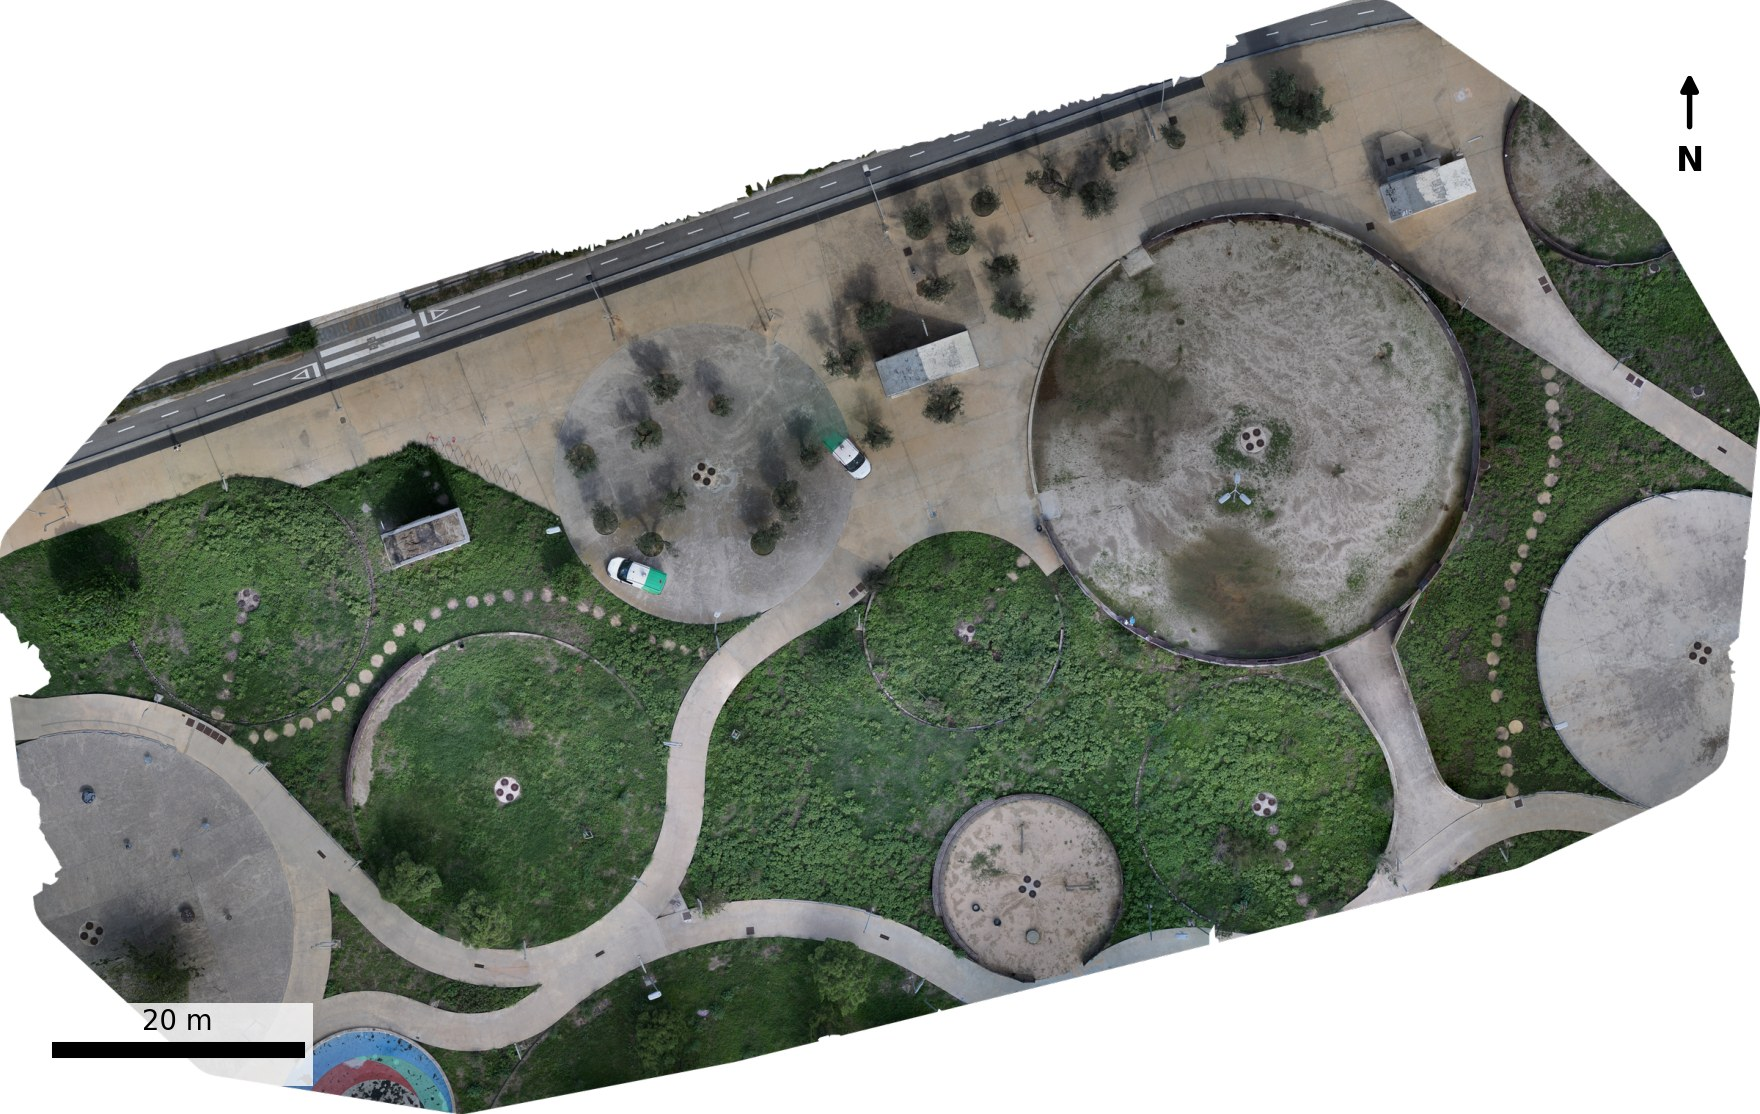
\includegraphics[width=\textwidth]{img/vol5_ortofoto.jpg}
    \caption{Ortofoto del vol de prova 5 (1~cm/px, EPSG:32631), processat amb posicions corregides pel retard de l'obturador.}
    \label{fig:vol5-ortofoto}
\end{figure}

L'ortofoto (14.084~$\times$~8.918~px a 1~cm/px) és coherent: sense costures ni deformació en forma de bol, amb vials i rotondes coherents i nítida a escala 1:1 (juntes de formigó, fulles individuals). El DSM (7.041~$\times$~4.458~px a 2~cm/px) és net a l'interior (edificis plans, arbres com a relleu); la primera i l'última passada i els extrems mostren estries per haver-hi poques vistes, de manera que convé retallar el DSM al polígon d'interès o ampliar el pla de vol un \emph{footprint} més enllà de la zona.

\begin{figure}[H]
    \centering
    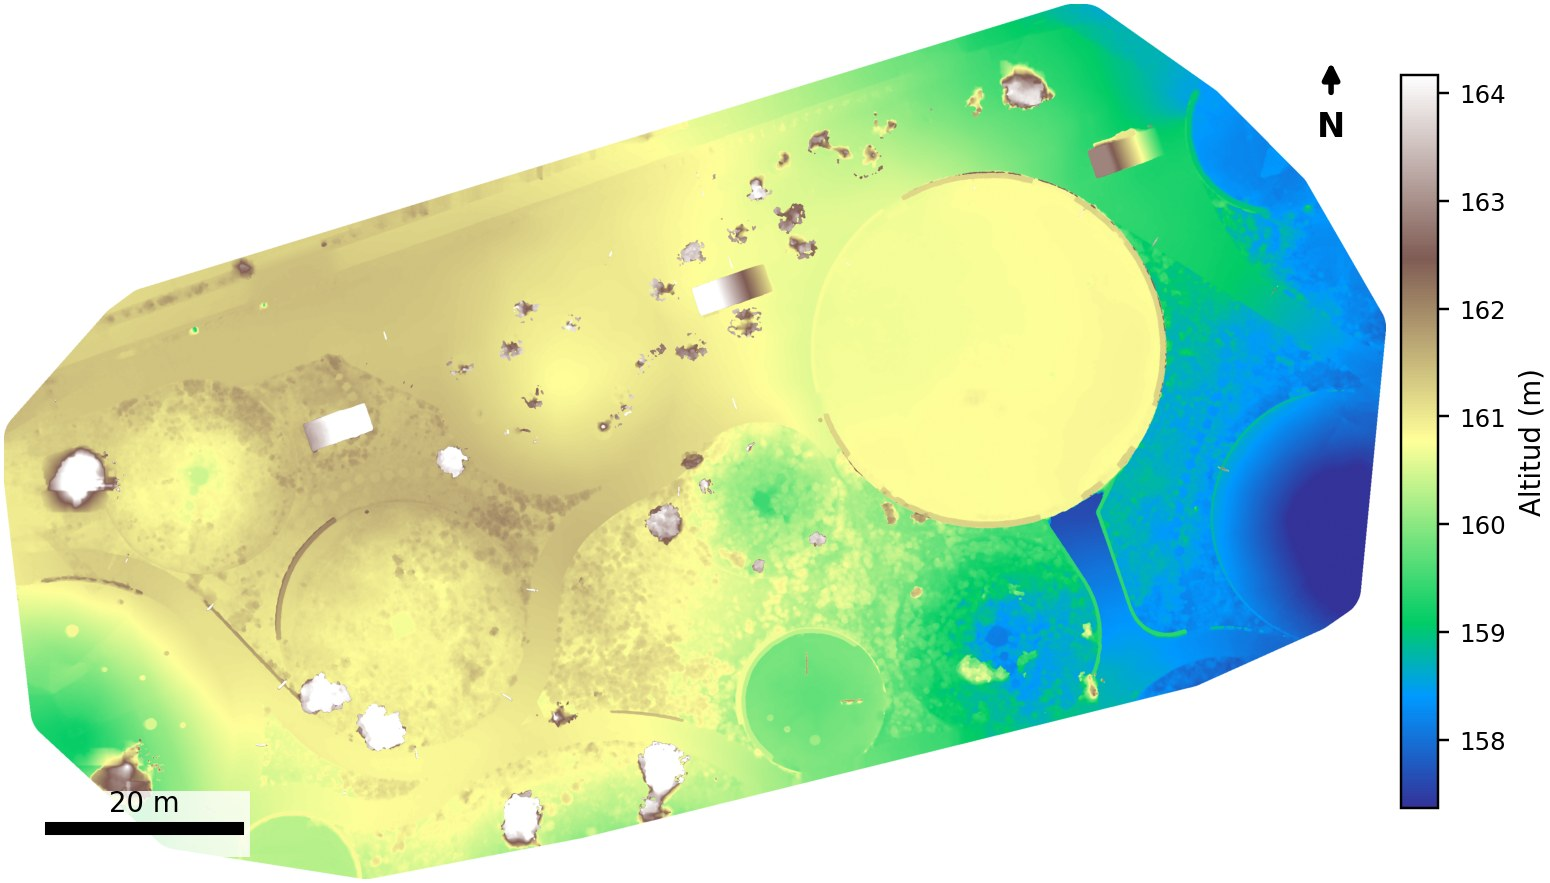
\includegraphics[width=\textwidth]{img/vol5_dsm.jpg}
    \caption{Model digital de superfície del vol de prova 5 (2~cm/px). Els buits blancs són copes d'arbres per sobre del rang de la paleta.}
    \label{fig:vol5-dsm}
\end{figure}

\section{Vol de prova 6 -- camp (13 d'octubre de 2026)}
\label{sec:vol6}

\subsection{Equip i vols}

El vol de prova 6 consta de dos vols a $\sim$50~m (àrea de $\sim$180~$\times$~150~m) amb el mateix dron i càmera que el 5 i amb els paràmetres de bateria ja calibrats. S'hi va validar el \emph{feedback} de la sabata (\texttt{CAM}) i la planificació a 50~m. Es van fer a l'alba, amb el sol entre $-3^{\circ}$ i $+1^{\circ}$ sobre l'horitzó, de manera que les fotografies van sortir molt fosques.

\begin{table}[H]
    \centering
    \caption{Registre dels dos vols del vol de prova 6}
    \label{tab:vol6-logs}
    \small
    \begin{tabular}{lcc}
        \toprule
        & Vol 1 (07:46) & Vol 2 (07:57) \\
        \midrule
        mAh consumits (\texttt{CurrTot} / integral) & 2.326 / 2.306 & 2.434 / 2.426 \\
        Motors en marxa & 5,5~min & 11,3~min (dos armats) \\
        Tensió inicial / mínima / final & 24,65 / 21,25 / 21,95~V & 24,73 / 21,13 / 21,95~V \\
        Corrent mitjà / màxim & 25 / 56~A & 22 / 58~A \\
        \emph{Failsafe} de bateria baixa & 268~s, 21,52~V, 1.887~mAh & 635~s, 21,48~V, 2.012~mAh \\
        Dispars \texttt{TRIG} / \texttt{CAM} / fotos & 94 / 93 / 94 & 110 / 110 / 110 \\
        \bottomrule
    \end{tabular}
\end{table}

\begin{itemize}
    \item \textbf{Bateria.} Els dos vols acaben per \emph{failsafe} de bateria baixa quan només s'ha gastat el 47--50~\% dels 4.000~mAh: la tensió instantània cau per sota de 21,6~V sota càrrega (\texttt{BATT\_FS\_VOLTSRC=0}). Cal comparar els mAh amb el que torna el carregador.
    \item \textbf{Exposició.} 1/1600~s, f/5,6, ISO 1600 (sostre de l'ISO automàtic): les fotografies queden unes 6~\emph{stops} subexposades, i la llum de l'escena és de 8,5--11,9~\emph{stops} per sota de la del vol 5 (sol a 40$^{\circ}$). El marge màxim de la càmera és de 5,7~\emph{stops}. No és cap avaria: és una limitació de llum.
    \item \textbf{Feedback.} Amb \texttt{TRIG}, \texttt{CAM} i fotografies en proporció 1:1 (110 de 110 al vol 2), l'aparellament es fa per instant. Hi ha una foto manual sense \texttt{TRIG} i un \texttt{TRIG} sense foto.
\end{itemize}

\pendent{Repetir aquest vol amb el sol a més de 10--15$^{\circ}$, que és la condició que el fa aprofitable (el lot actual només serveix de prova).}

\subsection{Processat del vol 2}

El vol 1 no és aprofitable (el guany digital $\times 551$ no recupera senyal: 2 coincidències entre fotos consecutives, igual que el soroll). Del vol 2 es van processar les 110 fotografies amb un guany lineal de $\times 2$ a $\times 97$ (mediana $\times 49$); \textbf{la geometria és vàlida, però els colors i els valors radiomètrics no ho són} (to verd-blavós, soroll alt), per la qual cosa aquest lot no serveix per a color ni índexs de vegetació.

\begin{table}[H]
    \centering
    \caption{Resultats del processat del vol 2 del vol de prova 6}
    \label{tab:vol6-resultats}
    \begin{tabular}{ll}
        \toprule
        Concepte & Valor \\
        \midrule
        Fotos reconstruïdes & 110 de 110 (1 component) \\
        Punts del model dispers / observacions & 101.094 / 354.361 \\
        Error de reprojecció & 1,82~px \\
        GSD mitjà / àrea reconstruïda & 0,743~cm/px / 30.626~m\textsuperscript{2} \\
        Núvol de punts dens & 27.207.845 punts \\
        Calibració de la càmera & focal 25,79~mm \\
        Diferència model--GPS (E / N / vert.) & 0,30 / 0,32 / 0,30~m; CE90 0,57~m, LE90 0,27~m \\
        Resolució d'ortofoto / DSM & 3~cm/px / 5~cm/px \\
        Temps de processat & 29~min 42~s \\
        \bottomrule
    \end{tabular}
\end{table}

La qualitat és inferior a la del vol 5 (reprojecció de 1,82~px davant de 0,90~px): és coherent amb el soroll de les imatges, que fa preferir una resolució de treball més gran (3~cm/px). L'ortofoto (7.799~$\times$~7.071~px) mostra el camp, els camins, la corba del camí i un vehicle blanc reconeixibles, amb to verd-blavós i soroll visibles i un contorn oest irregular. El DSM (4.679~$\times$~4.242~px) és detallat a l'interior (solcs, rodades) i té estries i una quadrícula d'interpolació a la vora oest i nord-oest.

\begin{figure}[H]
    \centering
    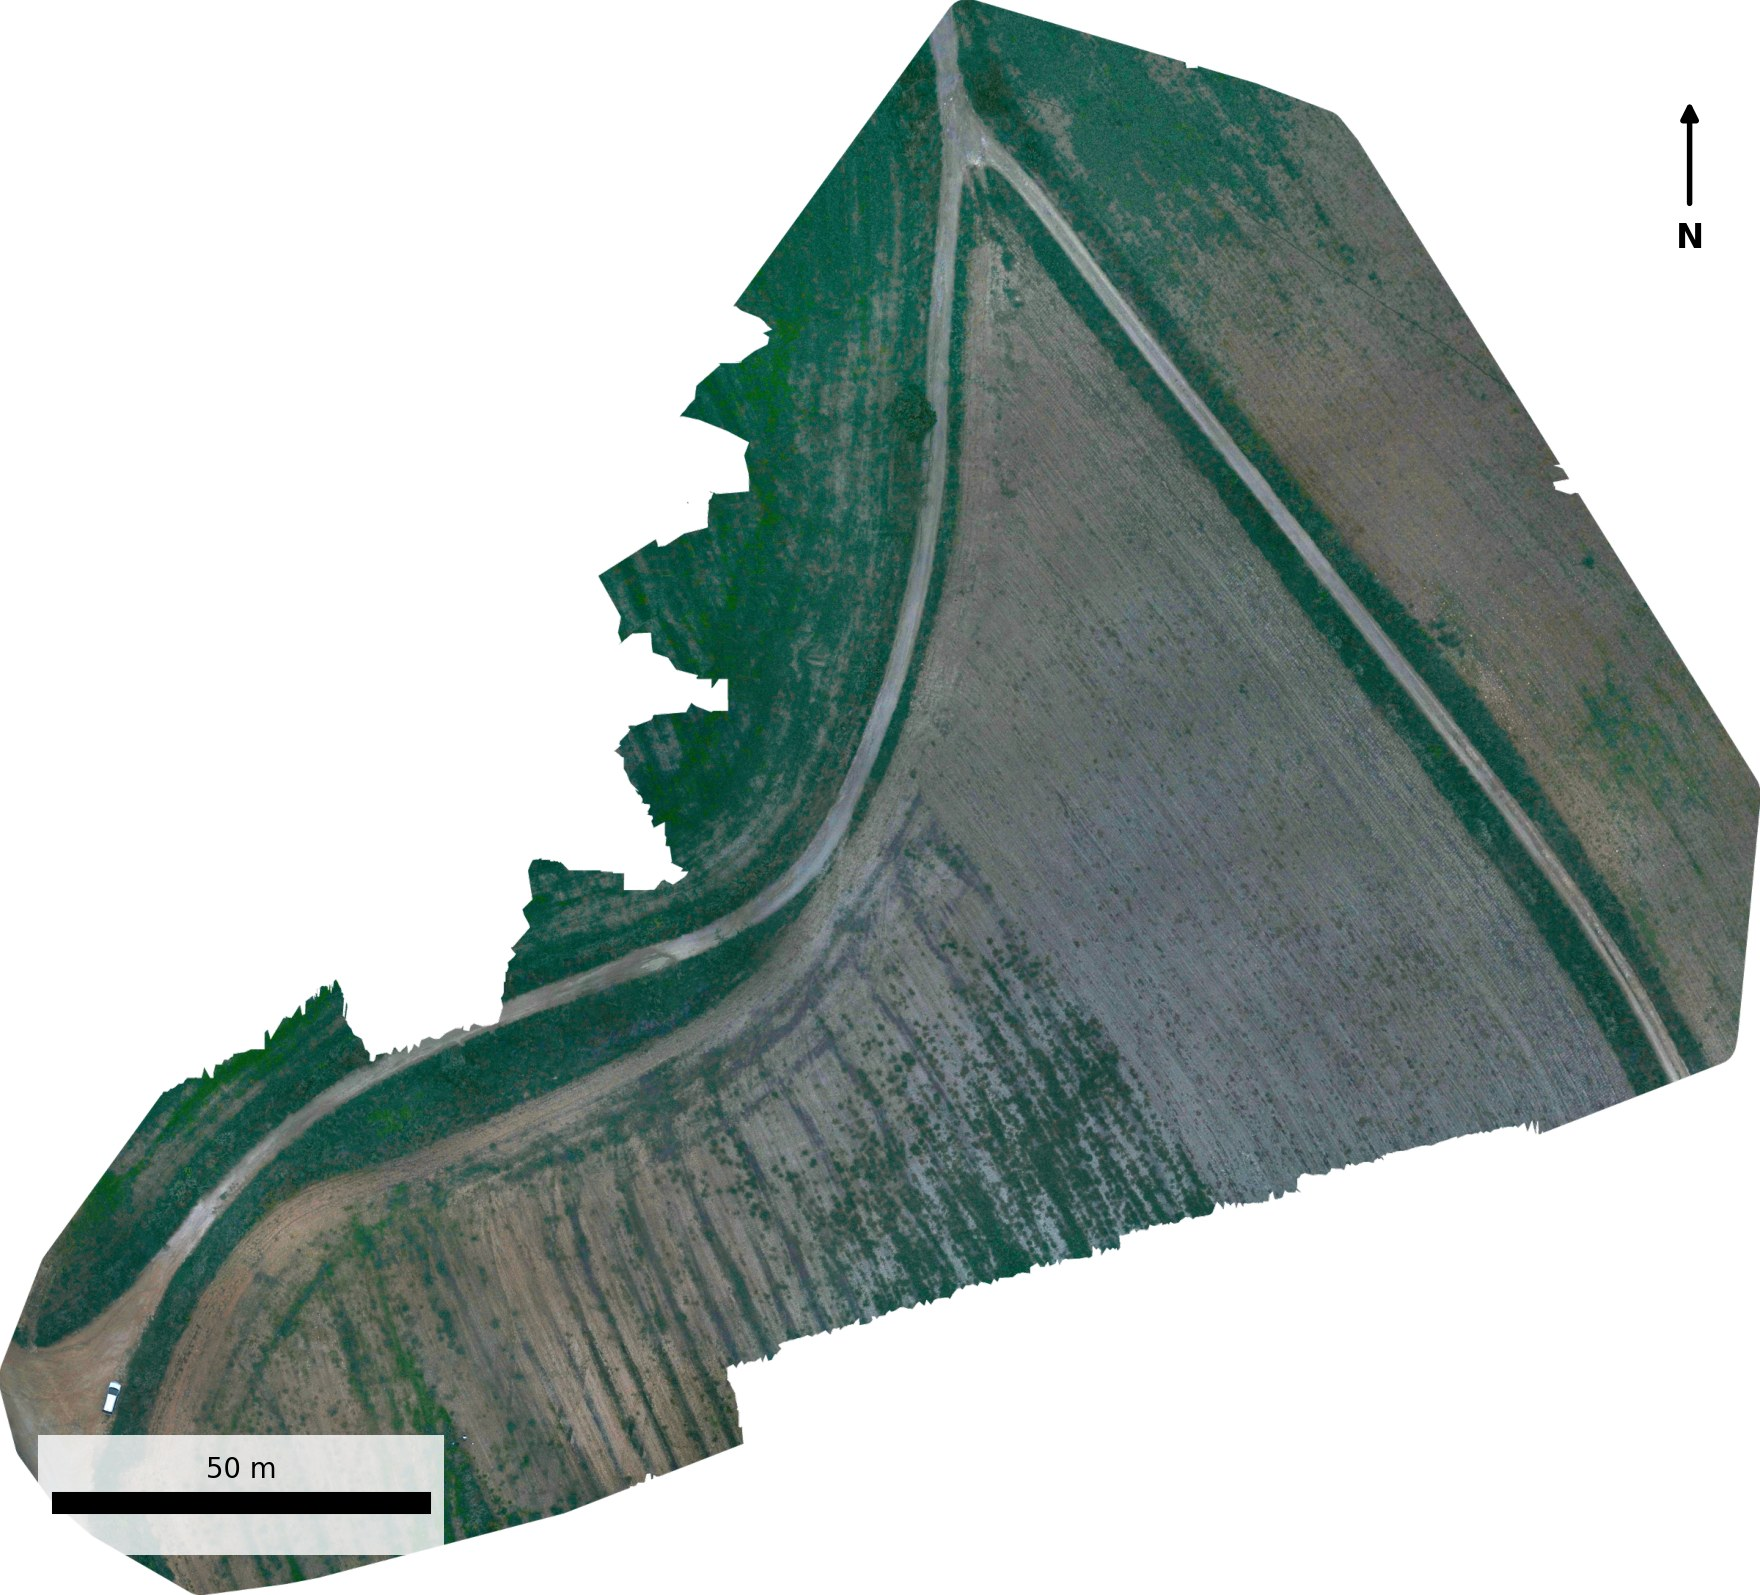
\includegraphics[width=0.85\textwidth]{img/vol6_ortofoto.jpg}
    \caption{Ortofoto del vol 2 de la prova 6 (3~cm/px). Les imatges s'han realçat digitalment: només la geometria és vàlida, no el color.}
    \label{fig:vol6-ortofoto}
\end{figure}

\begin{figure}[H]
    \centering
    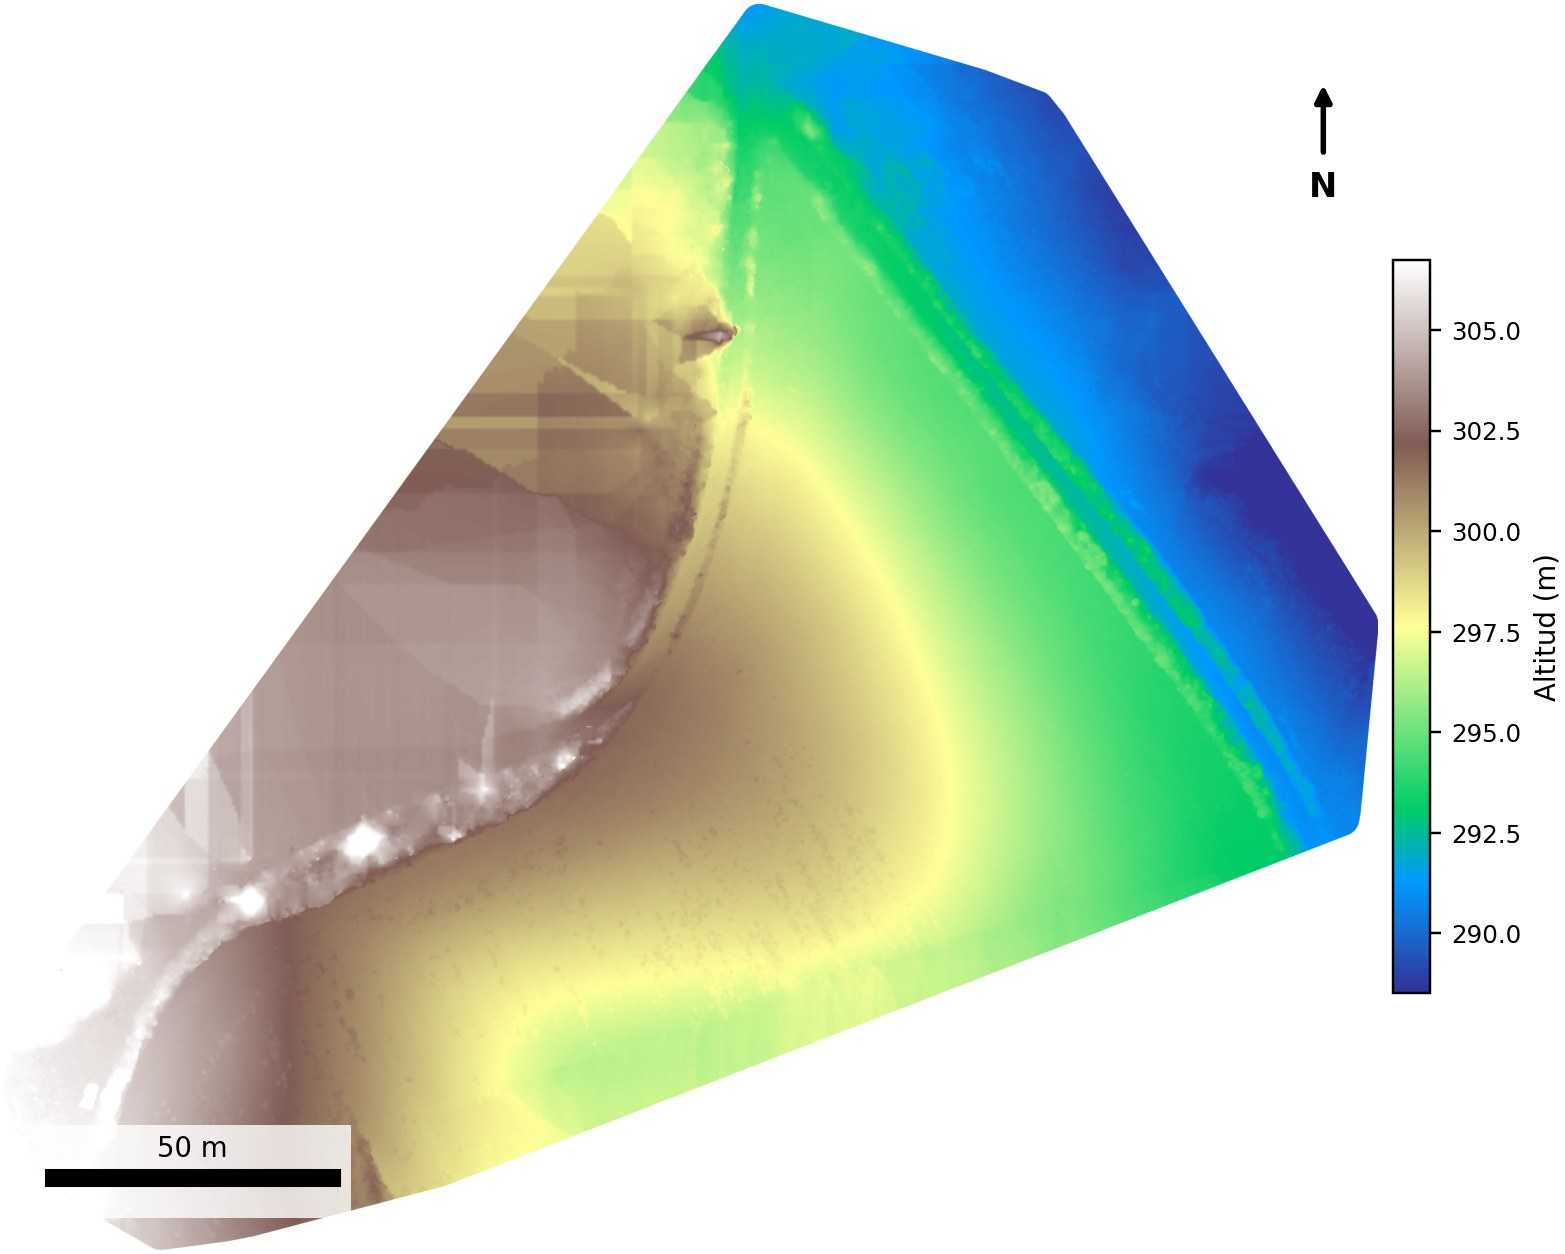
\includegraphics[width=0.85\textwidth]{img/vol6_dsm.jpg}
    \caption{Model digital de superfície del vol 2 de la prova 6 (5~cm/px).}
    \label{fig:vol6-dsm}
\end{figure}

\section{Retard de l'obturador}
\label{sec:retard-obturador}

L'ordre de dispar del controlador i l'exposició real no coincideixen: entre ells hi ha el retard del MAP2, de la càmera i, possiblement, el de la posició GPS/EKF. Com que el dron es mou a $\sim$5~m/s, un retard de 0,27~s equival a $\sim$1,3~m de desplaçament, molt per sobre de la precisió centimètrica buscada.

\subsection{Mètode}

Per a cada foto es compara la posició GPS del \emph{log} amb la posició de càmera reconstruïda pel model fotogramètric. Si el retard és $\tau$, el residu GPS $-$ model val $-v\tau$: té signe oposat a les passades d'anada i de tornada i un desplaçament global proper a zero, cosa que el distingeix d'un error sistemàtic de georeferenciació.

\subsection{Resultats}

\begin{table}[H]
    \centering
    \caption{Estimacions del retard de l'obturador}
    \label{tab:retard}
    \small
    \begin{tabular}{P{5.2cm}P{4.2cm}P{4.6cm}}
        \toprule
        Mesura & Retard & Observacions \\
        \midrule
        Vol 5, posicions \texttt{TRIG} & $\tau = 0{,}268 \pm 0{,}009$~s & ENE 0,277~$\pm$~0,007; WSW 0,267~$\pm$~0,014 \\
        Vol 5 amb posicions corregides & residual $0{,}004 \pm 0{,}007$~s & Residu horitzontal mediana 1,38~m $\rightarrow$ 0,35--0,49~m \\
        Vol 6, \texttt{TRIG}$\rightarrow$\texttt{CAM} & mediana 0,34~s (0,11--0,40) & Mesurat directament al \emph{log} \\
        Vol 6, posicions \texttt{CAM} & residual $-0{,}056 \pm 0{,}011$~s & La posició \texttt{CAM} va $\sim$56~ms per davant de l'exposició \\
        Vol 6, \texttt{TRIG}$\rightarrow$exposició & $0{,}34 - 0{,}056 \approx 0{,}28$~s & D'acord amb el vol 5 per un camí independent \\
        Banc, comandament$\rightarrow$obturador & 0,12--0,19~s & No explica tot el retard en vol \\
        \bottomrule
    \end{tabular}
\end{table}

Dos mètodes independents --~el residu fotogramètric del vol 5 i la combinació de \texttt{TRIG}, \texttt{CAM} i residu del vol 6~-- coincideixen en 0,27--0,28~s. És un retard \emph{efectiu}: suma el de l'obturador i, possiblement, el de la posició GPS/EKF, i un desplaçament fix de l'antena respecte a la càmera cap endavant es confon amb ell (si es deixa com a incògnita, el retard surt 0,34~$\pm$~0,03~s i el desplaçament 0,32~$\pm$~0,16~m, i no es poden separar). El retard del banc no explica tot el valor en vol; no es pot separar sense \emph{feedback}.

\subsection{Conseqüències per al geoetiquetat}

Amb \emph{feedback} (\texttt{CAM}), la posició és la de l'exposició real i només queda un retard residual de $-0{,}056$~s ($\sim$0,3~m a 5~m/s), que es pot compensar. Sense \emph{feedback} cal desplaçar la posició $v\cdot\tau$ amb $\tau \approx 0{,}27$~s i precisions per foto més amples. Aquest és el motiu pel qual el \emph{feedback} de la sabata és obligatori per a precisió centimètrica (\cref{sec:decisions}).

\section{Balanç dels vols de prova}
\label{sec:balanc-vols}

\textbf{Què ha funcionat.}
\begin{itemize}
    \item La cadena completa, de la planificació al DSM, amb RTK Fixed durant tot el vol als dos receptors i \emph{yaw} GNSS vàlid.
    \item Una geometria de qualitat fotogramètrica: reprojecció de 0,90~px, 118 de 118 fotos reconstruïdes i un GSD (0,451~cm/px) coherent amb l'alçada de vol i la focal calibrada (\cref{sec:planificacio-vol}).
    \item El \emph{feedback} de la sabata (110 de 110 al vol 6) i la quantificació independent del retard de l'obturador.
\end{itemize}

\textbf{Limitacions.}
\begin{itemize}
    \item No hi ha punts de control ni de comprovació: no es pot afirmar una precisió absoluta. Les xifres model--GPS són de coherència interna.
    \item La posició absoluta depèn de la base RTK, que en aquests vols va fer un \emph{survey-in} a cada sessió amb l'antena a 122~cm (\cref{subsec:muntatge-base}). No es va registrar la posició resultant, i l'error absolut és de l'ordre de metres, comú a tot el vol.
    \item Del vol 5 no es disposa de les condicions meteorològiques, la massa en vol ni la bateria utilitzada: el \emph{log} i les fotografies són l'únic registre.
    \item La llum limita l'operació: cal volar amb el sol a més de 10--15$^{\circ}$ (o, amb poca llum, 1/800~s, f/4 i ISO 3200 al límit).
    \item L'autonomia és curta: els \emph{failsafes} de bateria baixa actuen a mig consum per la caiguda de tensió sota càrrega (\cref{sec:autonomia}).
    \item El DSM presenta estries a la perifèria: cal ampliar el pla de vol un \emph{footprint} més enllà de la zona d'interès.
\end{itemize}

\textbf{Pròxims passos.} Repetir el vol de camp amb el sol alt, mesurar punts de control i de comprovació a terra per establir la precisió absoluta, reestimar el retard amb \emph{feedback} i millorar l'autonomia (\cref{sec:propulsor}). La llista completa de tasques pendents és a \cref{sec:pendents-proves-vol}.

\pendent{La precisió absoluta (horitzontal i vertical) del producte final continua sense mesurar: tots els errors d'aquest capítol són de coherència interna.}


\backmatter
\printbibliography[title={Referències}]

\end{document}
